    \documentclass[
        fleqn,
        usenatbib,
    ]{mnras}
    \usepackage{
        amsmath,
        amssymb,
        newtxtext,
        newtxmath,
        ae, aecompl,
        graphicx,
        booktabs,
    }
    \usepackage[T1]{fontenc}
    \usepackage[
        labelfont=bf, % caption names are labeled in bold
        font=scriptsize % smaller font for captions
    ]{caption}
    \usepackage[font=scriptsize]{subcaption} % subfigures
    \captionsetup{compatibility=false}

    \newcommand*{\rd}[2]{\frac{\mathrm{d}#1}{\mathrm{d}#2}}
    \newcommand*{\pd}[2]{\frac{\partial#1}{\partial#2}}
    \newcommand*{\md}[2]{\frac{\mathrm{D}#1}{\mathrm{D}#2}}
    \newcommand*{\at}[1]{\left.#1\right|}
    \newcommand*{\abs}[1]{\left|#1\right|}
    \newcommand*{\ev}[1]{\langle#1\rangle}
    \newcommand*{\p}[1]{\left(#1\right)}
    \newcommand*{\s}[1]{\left[#1\right]}
    \newcommand*{\z}[1]{\left\{#1\right\}}
    \DeclareMathOperator*{\argmin}{argmin}
    \DeclareMathOperator*{\argmax}{argmax}
    \DeclareMathOperator*{\med}{med}

\title[Cassini State Capture]{Cassini State Capture}
\author[Y. Su et\ al.]{
Yubo Su$^1$,
Dong Lai$^1$
\\
$^1$ Cornell Center for Astrophysics and Planetary Science, Department of
Astronomy, Cornell University, Ithaca, NY 14853, USA
}

\date{Accepted XXX\@. Received YYY\@; in original form ZZZ}

\pubyear{2019}

\begin{document}\label{firstpage}
\pagerange{\pageref{firstpage}--\pageref{lastpage}}
\renewcommand*{\sectionautorefname}{Section}
\maketitle

% TODO
% figure out whether can draw vertical lines on 3testo plots for regimes
% run simulations up to III -> III (not today)

\begin{abstract}
    Abstract
\end{abstract}

\begin{keywords}
planet--star interactions % chktex 8
\end{keywords}

\section{Introduction}

The primary result of our paper is \autoref{fig:nonad_3_ensemeble}.

\section{Equations}\label{s:eq}

Denote $\vec{s}$ spin of planet, $\vec{l}$ angular momentum of planet, and
$\vec{l}_d$ angular momentum of the surrounding disc. We approximate $S \ll L
\ll L_d$, so $\vec{l}_d$ is approximately constant. Much of this treatment
borrows from \citealp{anderson2018teeter} and \citealp{millholland_disk}. We
consider precession equations
\begin{align}
    \rd{\hat{s}}{t} &= \omega_{sl} \p{\hat{s} \cdot \hat{l}}
        \p{\hat{s} \times \hat{l}}\label{eq:dsdt}\\
    \rd{\hat{l}}{t} &= \omega_{ld}\p{\hat{l} \cdot \hat{l}_d}
        \p{\hat{l} \times \hat{l}_d},\label{eq:dldt}\\
\end{align}
where
\begin{align}
    \omega_{sl} &\equiv \frac{3k_{qp}}{2k_p} \frac{M_\star}{m_p}
        \p{\frac{R_p}{a_p}}^3 \Omega_p,\label{eq:wsl}\\
    \omega_{ld} &\equiv \frac{3M_d}{4M_\star}\p{\frac{a_p}{r_d}}^3 n
        .\label{eq:wld}
\end{align}
In \autoref{eq:wsl}, $k_{qp}$ and $k_p$ are related to the planet's quadrupole
moment and moment of inertia respectively \citep[see][]{lai2018}, $M_\star$ is
the mass of the host star, and $M_p, R_p, a_p, \Omega_p$ are the mass, radius,
semi-major axis and angular spin frequency of the planet respectively.
\autoref{eq:wld} is written for a disk of mass $M_d$ located at characteristic
distance $r_d$ from the host star \citep[see][for a power-law disk
profile]{millholland_disk}, $n \equiv \sqrt{GM_\star/a_p^3}$ is the planet's
orbital mean motion. The three angles formed by the three vectors are notated
\begin{align}
    \theta &\equiv \arccos \hat{s} \cdot \hat{l},\\
    \theta_{sd} &\equiv \arccos \hat{s} \cdot \hat{l}_d,\\
    I &\equiv \arccos \hat{l} \cdot \hat{l}_d.
\end{align}

We go to the corotating frame with $\hat{l}$ fixed such that $\hat{z} =
\hat{l}$ ($\theta$ is now conveniently also the polar component of $\hat{s}$).
The evolution of $\hat{s}$ in this corotating frame is governed by:
\begin{equation}
    \rd{\hat{s}}{t} = \alpha \p{\hat{s} \cdot \hat{l}}
            \p{\hat{s} \times \hat{l}}
        - \abs{g}\p{\hat{s} \times \hat{l}_d}.
\end{equation}
$\alpha = \omega_{sl} > 0, g \equiv -\omega_{ld}\cos I < 0$ follow traditional
sign conventions.

We divide through by $\alpha$ and define parameter $\eta$ and nondimensionalized
time $\tau$
\begin{align}
    \eta &\equiv \frac{\abs{g}}{\alpha}\label{eq:eta},\\
    \tau &\equiv \alpha t.
\end{align}
The redimensionalized equation of motion is then
\begin{equation}
    \rd{\hat{s}}{\tau} = \p{\hat{s} \cdot \hat{l}}
            \p{\hat{s} \times \hat{l}}
        - \eta\p{\hat{s} \times \hat{l}_d}. \label{eq:dsdt_base}
\end{equation}

Following~\cite{millholland_disk}, we allow $g$ to vary in time owing to a
disk with decaying mass
\begin{equation}
    M_d(t) = M_d(0)e^{-t/t_d}.
\end{equation}
As $\alpha$ is held constant, this equates to $\eta$ decaying as $\rd{\eta}{t} =
-\frac{\eta}{t_d}$ for some decay time $t_\eta$. We nondimensionalize by
defining $\epsilon \equiv \frac{1}{\alpha t_\eta}$, so
\begin{equation}
    \rd{\eta}{\tau} = -\epsilon \eta.\label{eq:deta_dt}
\end{equation}
Equations \autoref{eq:dsdt_base} and \autoref{eq:deta_dt} constitute our system
of study.

Finally, the Hamiltonian corresponding to the equation of motion
\autoref{eq:dsdt_base} is
\begin{equation}
    \mathcal{H}\p{\theta, \phi} = -\frac{1}{2}\p{\hat{s} \cdot \hat{l}}^2
        + \eta \p{\hat{s} \cdot \hat{l}_d}.\label{eq:H}
\end{equation}
Here, we adopt a spherical coordinate system where $\hat{l} = \hat{z}$ and
$\theta, \phi$ are the polar and azimuthal angle of $\hat{s}$. By convention, we
choose $\hat{l}_z$ at coordinates $\theta = I, \phi = \pi$, in which case the
Hamiltonian can be written
\begin{equation}
    \mathcal{H} = -\frac{1}{2}\cos^2\theta
        + \eta \p*{\cos \theta \cos I - \sin I \sin \theta \cos \phi}.
\end{equation}

Note that $\p{\cos \theta, \phi}$ form a canonically conjugate pair of variables
describing $\hat{s}$. The equations of motion for these variables can be derived
by taking derivatives of $\mathcal{H}$ given by \autoref{eq:H} and agree with
\autoref{eq:dsdt_base}:
\begin{subequations}\label{se:H_eom}
    \begin{align}
        \pd{\phi}{t} = \pd{\mathcal{H}}{(\cos\theta)}
            &= -\cos\theta + \eta\p{\cos I + \sin I \cot \theta \cos \phi},\\
        \pd{(\cos \theta)}{t} = -\pd{\mathcal{H}}{\phi}
            &= -\eta \sin I \sin \theta \sin \phi.
    \end{align}
\end{subequations}
While these equations are numerically stiff owing to the $\cot\theta$ term, they
are the most intuitive description for analytical work.

\subsection{Cassini States}\label{ss:cs}

Spin states satisfying $\rd{\hat{s}}{t} = 0$ are referred to as \emph{Cassini
States} (CSs). There are either two or four solutions, depending on the values
of $\eta, I$. Following standard convention and nomenclature (see
\autoref{fig:cs_locs}), CSs 1, 3, 4 have $\phi = 0, \theta < 0$ and CS2 has
$\phi = \pi, \theta > 0$. Of these, CSs 1, 2, 3 are stable while CS4 is
unstable.

When $\eta < \eta_c$, where
\begin{equation}
    \eta_c \equiv \p{\sin^{2/3}I + \cos^{2/3}I}^{-3/2},
\end{equation}
all four CSs exist, and when $\eta > \eta_c$, only CSs 2, 3 exist
\citep{henrard1987,ward2004I}. The CS obliquities as a function of $\eta$ are
provided in \autoref{fig:cs_locs}.
\begin{figure}
    \centering
    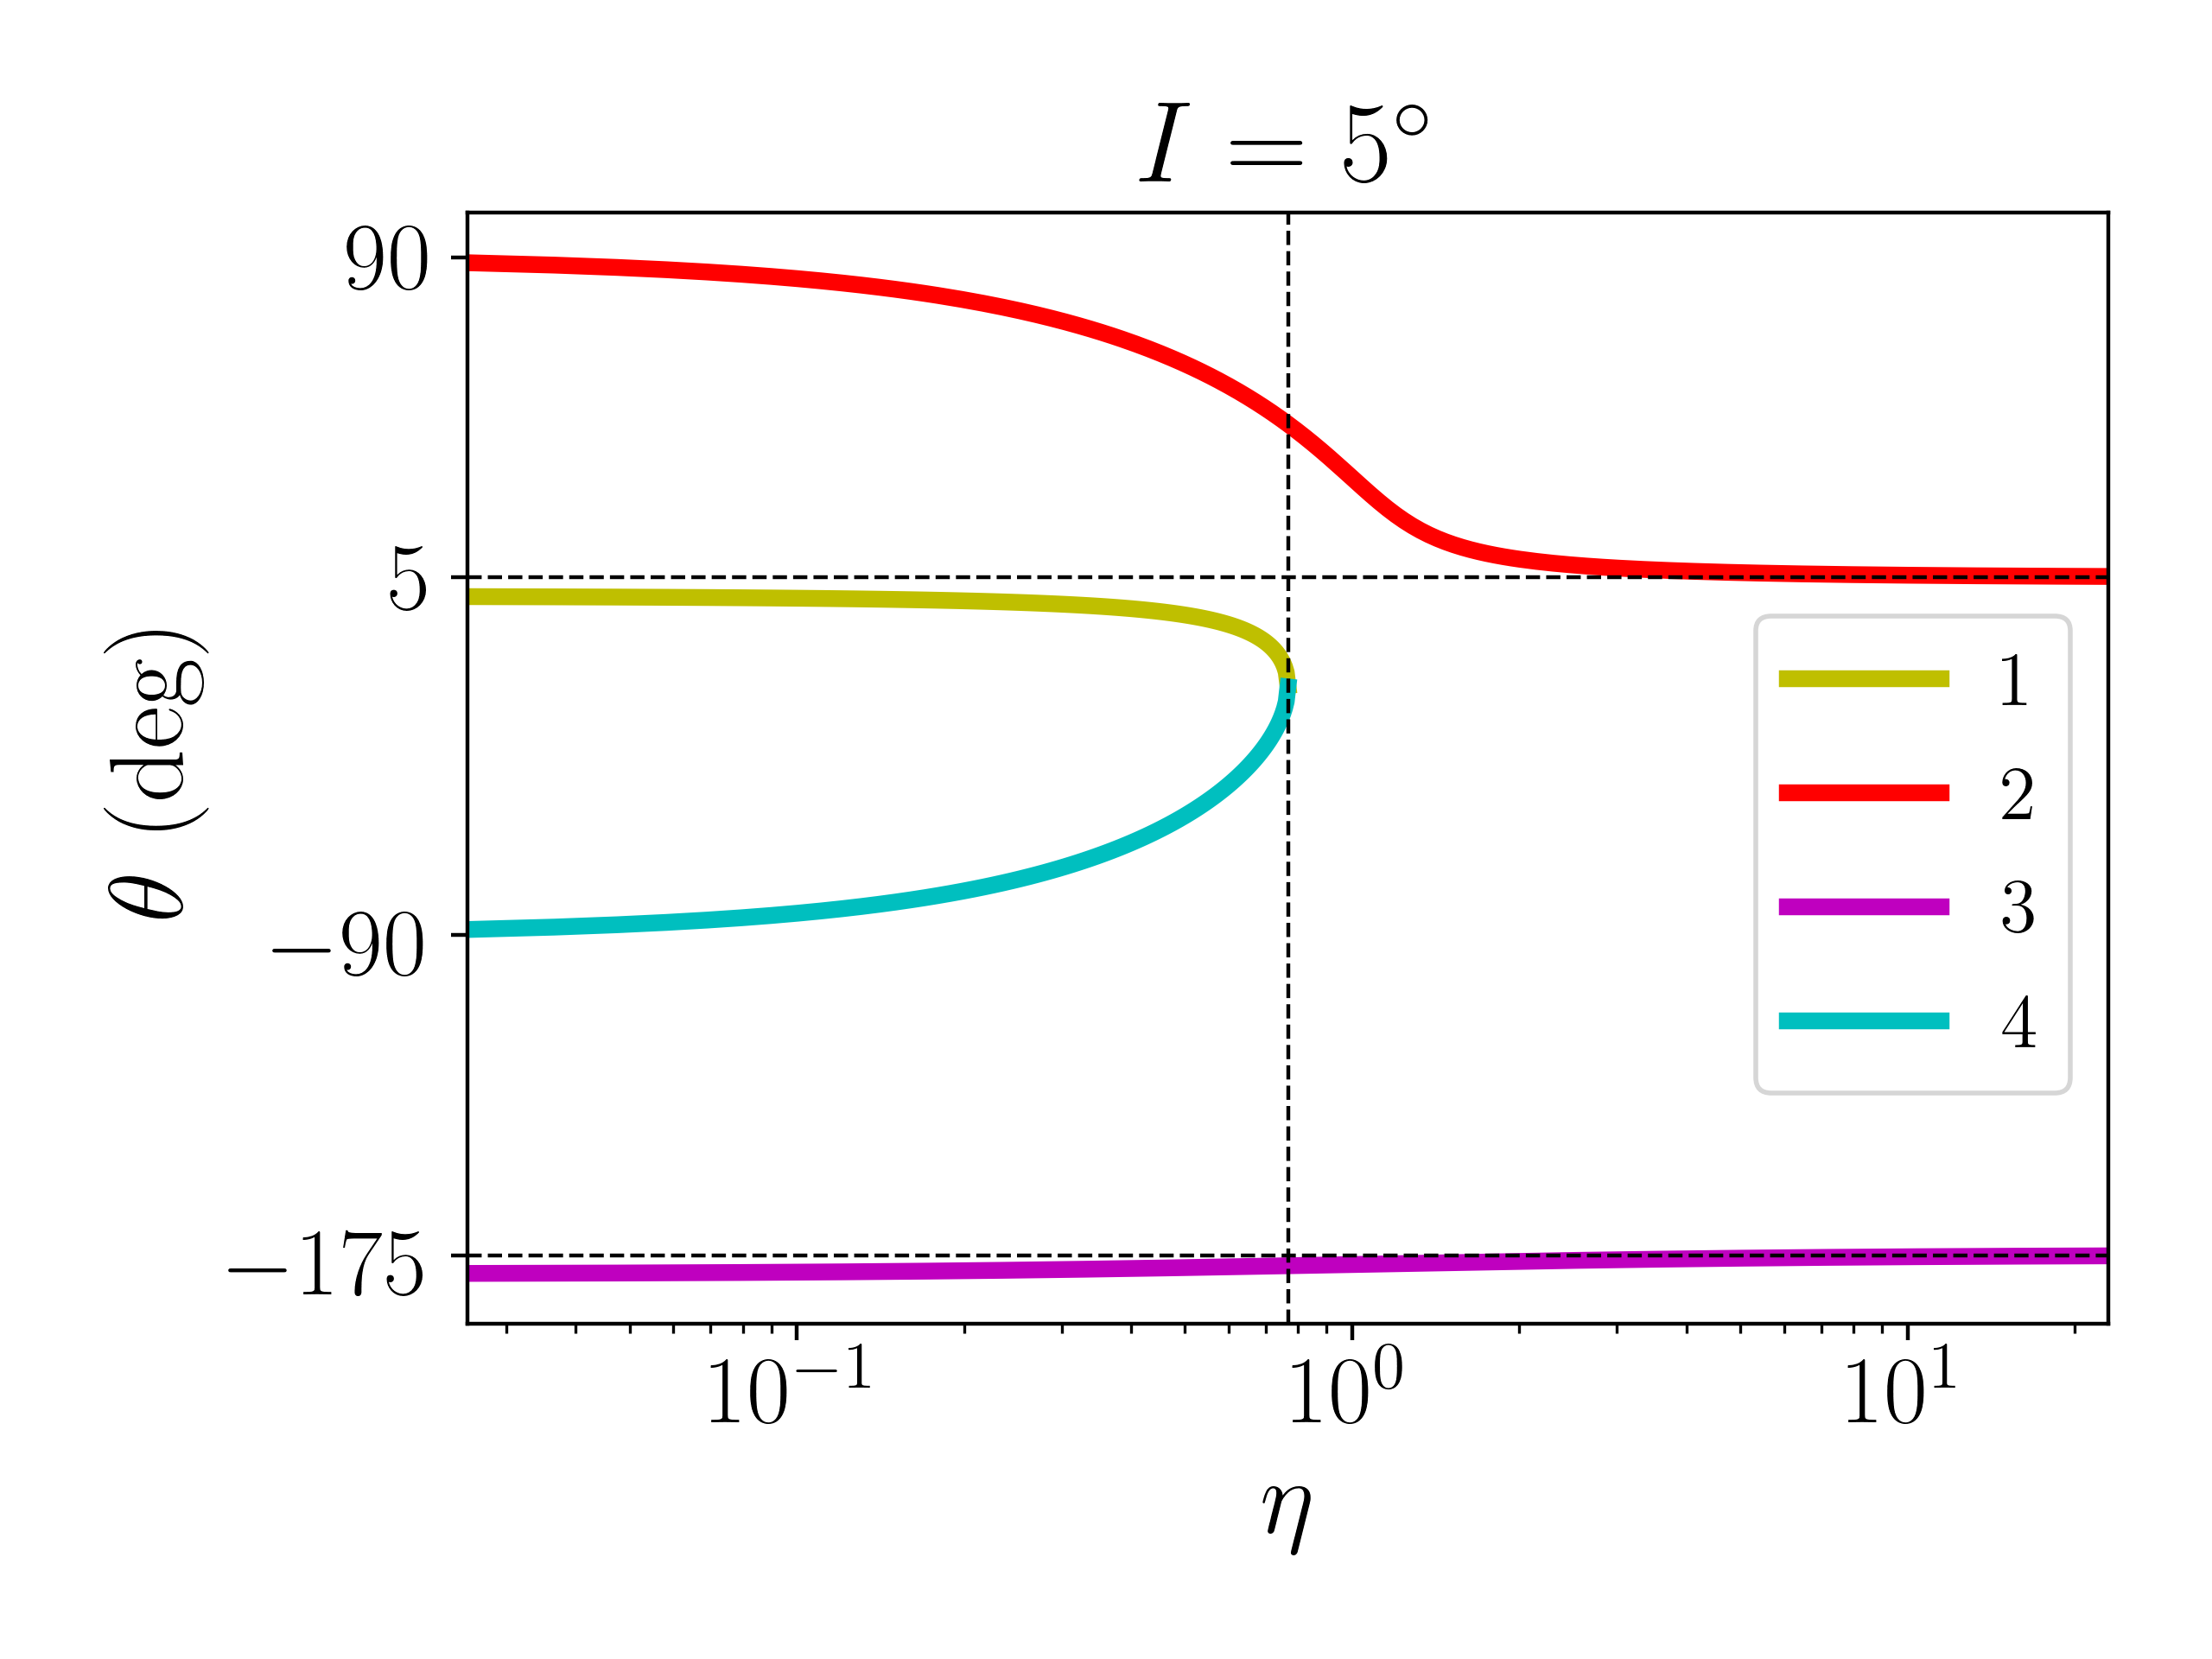
\includegraphics[width=\columnwidth]{../initial/99_misc/2_cs_locs.png}
    \caption{$\theta$ values of the Cassini states over time, following the same
    coloring scheme as \autoref{fig:eq_1contours}. Note that $\theta \in [-\pi,
    \pi]$ is the traditional definition of the polar angle
    \citep[see e.g.][]{colombo1966,peale1969,henrard1987}.}\label{fig:cs_locs}
\end{figure}

\subsection{Separatrix}

When $\eta < \eta_c$, CS4 exists and is a saddle point. All trajectories are
periodic with finite period except two critical trajectories asymptotic in the
past and future to CS4. Together, these two critical trajectories are referred
to as the \emph{separatrix} and divide phase space into three zones. The
separatrix, three zones, and their relations to the CSs are most clearly shown
via a contour plot of $\mathcal{H}\p{\phi, \cos \theta}$ in
\autoref{fig:eq_1contours}.
\begin{figure*}
    \centering
    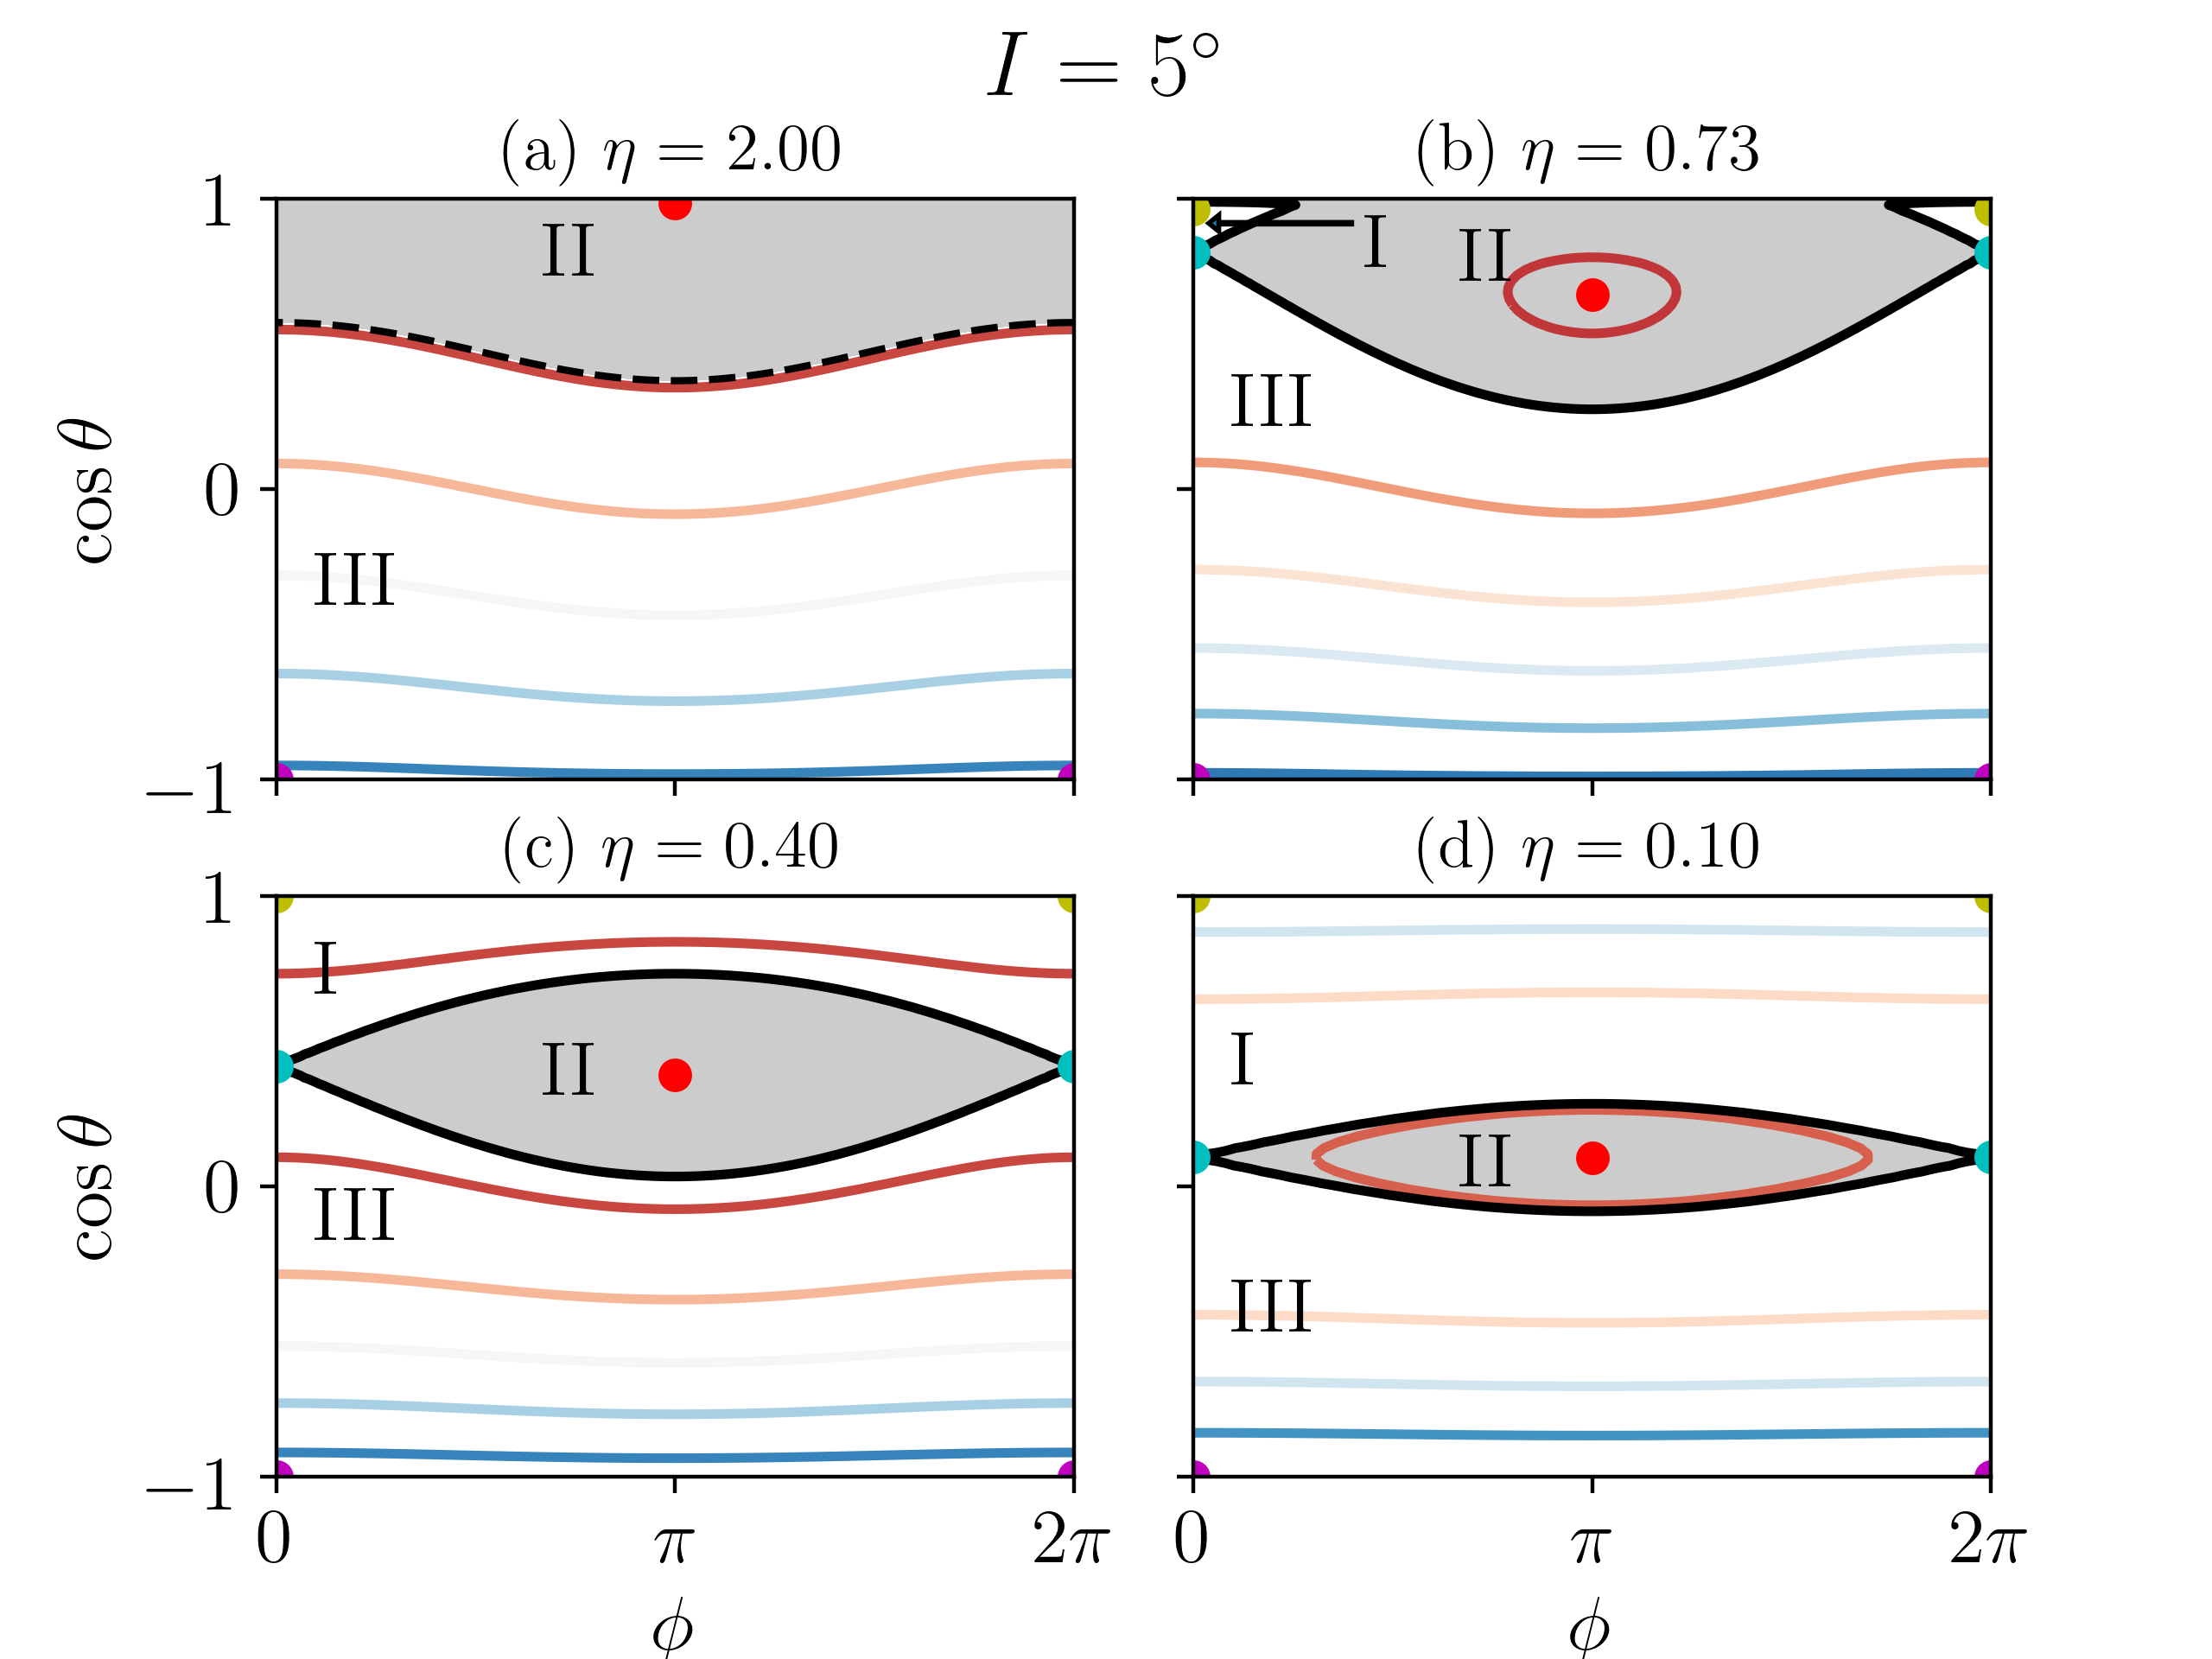
\includegraphics[width=0.8\textwidth]{../initial/0_eta/1contours_flip.png}
    \caption{Contour plot of $\mathcal{H}\p{\phi, \cos \theta}$, where warmer
    colors denote more positive values. The black solid line is the separatrix,
    which only exists for $\eta < \eta_c$. The three zones, divided by the
    separatrix, are labeled. The interior of the separatrix, shaded in grey, is
    formally only defined for $\eta < \eta_c$, but we may identify the phase
    space trajectories that flow into zone II when evolved forward in time; this
    is the shaded region in the top left plot, bounded by the dotted black
    line.}\label{fig:eq_1contours}
\end{figure*}

As trajectories of constant $\eta$ evolve along contours of constant
$\mathcal{H}$, it can be observed that trajectories in zone II librate about CS2
while those in zones I/III circulate.

The unsigned areas of the three zones are known exactly
\citep{henrard1987,ward2004I}. Defining
\begin{align*}
    z_0 &= \eta\cos I, &
    \chi &= \sqrt{-\frac{\tan^3\theta_4}{\tan I} - 1},\\
    \rho &= \chi \frac{\sin^2 \theta_4\cos \theta_4}{
        \chi^2 \cos^2\theta_4 + 1},&
    T &= 2\chi \frac{\cos \theta_4}{
        \chi^2 \cos^2\theta_4 - 1},\\
\end{align*}
the areas for $\eta < \eta_c$ are given by
\begin{subequations}\label{se:area_ward}
    \begin{align}
        A_{II} &= 8\rho + 4\arctan T - 8z_0 \arctan \frac{1}{\chi},\\
        A_I &= 2\pi\p{1 - z_0} - \frac{A_2}{2},\\
        A_{III} &= 2\pi\p{1 + z_0} - \frac{A_2}{2}.
    \end{align}
\end{subequations}
These are plotted as a function of $\eta$ in \autoref{fig:eq_areas}. Note that
the zones are not formally defined for $\eta > \eta_c$, but a natural extension
exists: evolve an initial point $p$ under adiabatic decrease of $\eta > \eta_c$
until the separatrix appears at $\eta = \eta_c$, then identify $p$ with the zone
it is in at $\eta_c$. Since phase space area is conserved under adiabatic
evolution, this implies $A_i\p{\eta > \eta_c} = A_i(\eta_c)$.
\begin{figure}
    \centering
    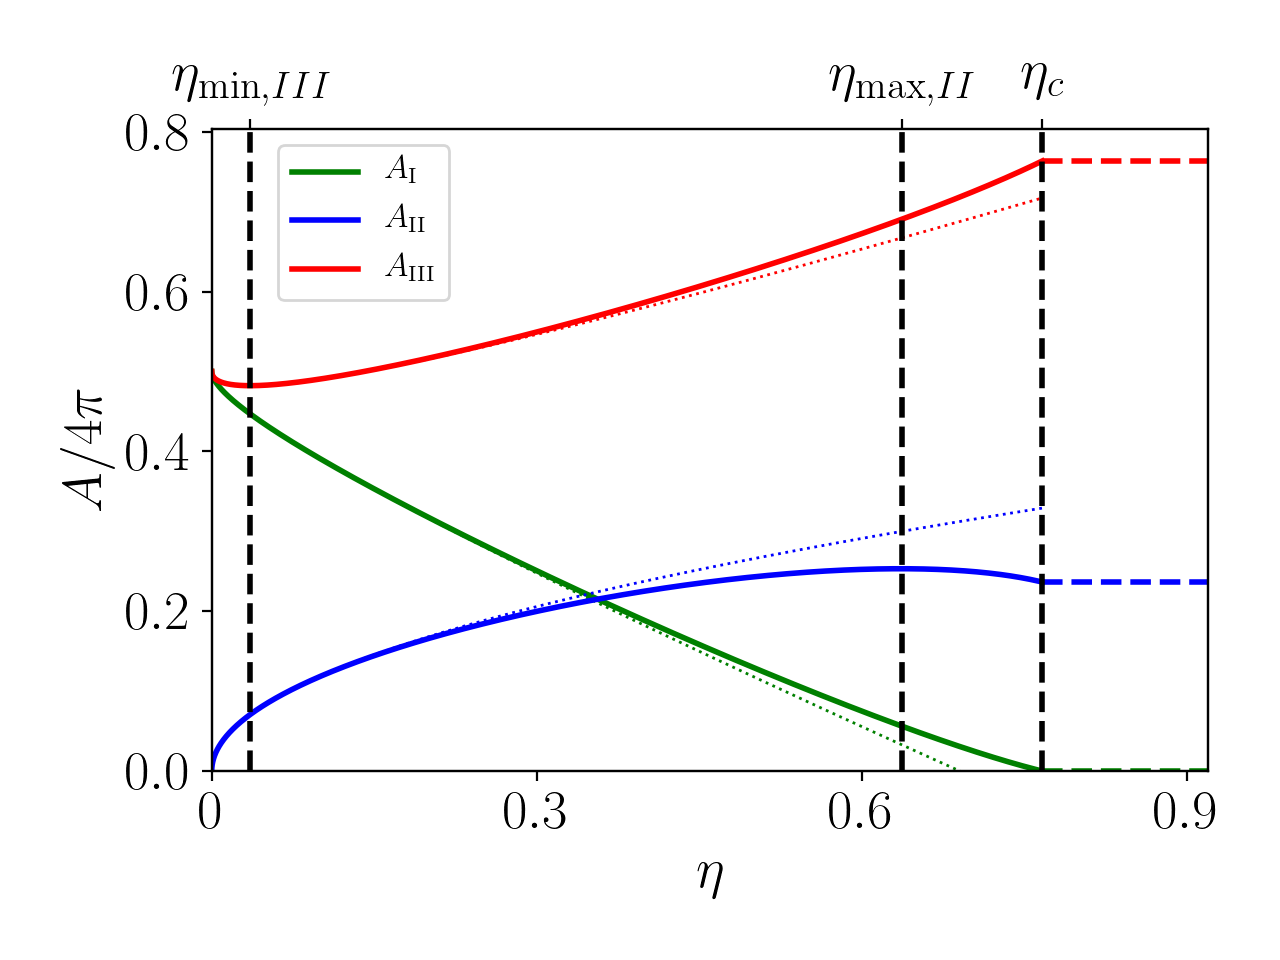
\includegraphics[width=\columnwidth]{../initial/99_misc/1_areas.png}
    \caption{Plot of fractional $A_{i}(\eta)$ as given by
    \autoref{se:area_ward}. Dotted lines correspond to small $\eta$
    approximations discussed in \autoref{ss:app_transition}. Dashed lines denote
    effective values of $A_{II}, A_{III}$ for $\eta > \eta_c$, denoting the
    area of points that would flow into either area under adiabatic decrease of
    $\eta$ to below $\eta_c$.}\label{fig:eq_areas}
\end{figure}

\section{Adiabatic Evolution}\label{s:ad}

As $\eta$ decreases, the trajectory generally encounters the separatrix at some
value $\eta_\star$ depending on its initial condition. If $\eta$ changes
sufficiently little during this separatrix-crossing orbit, the evolution of the
system is considered \emph{adiabatic}. In the truly adiabatic limit, $\epsilon
\to 0$; we use $\epsilon = 3 \times 10^{-4}$ unless otherwise noted.

One necessary criterion for adiabaticity is that the separatrix crossing
timescale be longer than the the resonant libration period \citep{ward2004I}.
The resonant libration period is just the libration period about CS2, which can
be found by linearizing \autoref{se:H_eom} about $\phi \approx \pi, \theta
\approx \theta_2$. The resulting criterion is
\begin{align}
    -\at{\frac{1}{\eta}\rd{\eta}{\tau}}_{cross} = \epsilon &\lesssim
            \frac{2\pi}{T_{lib}},\\
        &\lesssim \sqrt{\eta_\star\sin\theta \sin I
            \p{1 + \eta_\star \frac{\sin I}{\sin^3\theta}}}.\label{eq:ad_constr}
\end{align}
Note that this is a necessary but not sufficient criterion: the libration period
is longer for trajectories nearer the separatrix and diverges at the separatrix
for constant $\eta$. This formula also is in slight disagreement with that
presented in \citealt{millholland_disk}

\subsection{Separatrix Crossing and Evolutionary Tracks
}\label{ss:zone_transitions}

In the limit $\eta \to 0$, zone II disappears and all trajectories circulate at
constant final $\theta$ values, notated $\theta_f$. We run simulations that
terminate at $\eta = 10^{-{-3.5}}$ and measure $\theta_{f}$. We vary the initial
value of $\theta_{sd}$, notated $\theta_{sd, i}$, among our simulations.

In the absence of separatrix encounters, the enclosed phase space area $A \equiv
\oint \cos\theta \;\mathrm{d}\phi$ is an adiabatic invariant. Here, we adopt
convention where $A$ is a \emph{signed} area
\begin{equation}
    A = \oint \p{1 - \cos \theta}\;\mathrm{d}\phi.
\end{equation}
This has the advantage of (i) having a removable singularity when the trajectory
crosses $\cos \theta = 1$, and (ii) being easily expressible as combinations of
the $A_i$ of \autoref{se:area_ward}. The bounds of the integral are either a
libration ($\phi$ returns to its original value with the same $\dot{q\phi}$
sign) or circulation cycle ($\phi$ advances to $\phi \pm 2\pi$). Note lastly
that $A$ has simple physical interpretation of are enclosed on the unit sphere
by $\hat{s}$ over one cycle measured relative to $+\hat{z}$:
\begin{equation*}
    \int \int\limits_{\cos \theta(\phi)}^1
        \mathrm{d}\cos\theta\;\mathrm{d}\phi = \int \p{1 - \cos \theta(\phi)}
            \;\mathrm{d}\phi.
\end{equation*}

When a trajectory encounters the separatrix, $A$ will change discontinuously as
the trajectory moves between zones, but its change is easily understood
\citep{henrard1982}. We can classify trajectories by the separatrix encounters
they undergo. Initially, in the $\eta > \eta_c$ regime, only zones $II, III$
exist. Conversely, at the end of the simulation when $\eta \to 0$, only zones
$I, III$ exist. Most simply, one might expect four sequences of transitions
between zones (we call these dynamical ``tracks'') to manifest: from one of
$\z{I, III}$ to one of $\z{II, III}$. In addition to these four tracks, a
fifth track $III \to II \to I$ is observed.

Beyond simply identifying the possible tracks, we may clearly delineate the
initial conditions for which each track can be encountered. Separatrix crossing
is a probabilistic process whose outcomes are well understood by
\citealp{henrard1982,henrard1987}. Their resultss may be simply summarized as
follows: if a zone $i$ is shrinking and zone $j$ is expanding, the probability
of transition from zone $i$ to zone $j$ is given
\begin{equation}
    \Pr_{i \Rightarrow j} = -\frac{\pd{A_j}{t}}{ \pd{A_i}{t}}
        = -\frac{\pd{A_j}{\eta}}{ \pd{A_i}{\eta}}\label{eq:henrard_hop}
\end{equation}
This can be used directly in conjunction with \autoref{se:area_ward} to
understand for what initial conditions each track can be observed and with what
probabilities.

Below, we will describe the evolution of $A$ throughout each of the five tracks,
as well as determine the initial conditions and probabilities associated with
each track:
\begin{itemize}
    \item $II \to I$ --- This track is depicted in \autoref{fig:ad_21}.
        $\hat{s}$ starts librating about CS2 in zone II, enclosing some initial
        phase space area $A_i$. The trajectory is able to librate without
        separatrix encounter until $A_{II}(\eta_\star) = A_i$. At this point, as
        the trajectory transitions to a circulating trajectory in zone I
        immediately bordering the separatrix, it will encompass
        $-A_I(\eta_\star)$ phase space area. Conservation of phase space area
        then predicts that as $\eta \to 0$, the final enclosed phase space area
        will still be $A_f = -A_I$, and the final obliquity $\theta_f$ must be
        given by
        \begin{equation}
            2\pi\p{1 - \cos \theta_f} = A_f. \label{eq:qfaf}
        \end{equation}

        This transition can only occur when the initial condition begins in zone
        II, requiring $A_i < A_{II}(\eta_c)$, where $A_{II}(\eta_c)$ is known in
        closed form \citep{ward2004I}
        \begin{equation}
            A_{II}\p{\eta_c} = 4\pi \s{
                1 - \p{1 + \tan^{2/3}I}^{-3/2}}.
        \end{equation}
        Then, at some known $\eta_\star$ satisfying $A_{II}(\eta_\star) = A_i$,
        the trajectory is ejected from the separatrix and enters zone I with
        probability
        \begin{equation}
            \Pr_{II \to I} = -\at{\frac{\pd{A_I}{\eta}}{\pd{A_{II}}{\eta}}}
                _{\eta_\star}.
        \end{equation}
        Note that since $\pd{A_i}{\eta} < 0$ everywhere, while
        $\pd{A_{II}}{\eta} > 0$ at all possible $\eta_\star$ for an initial
        condition starting in zone II, this track always has nonzero
        probability.

    \item $II \to III$ --- This track is depicted in \autoref{fig:ad_23}. The
        only difference from the previous track is that, upon separatrix
        encounter, the trajectory follows the circulating trajectory in zone III
        bordering the separatrix, upon which it will encompass $A_f =
        A_I(\eta_\star) + A_{II}(\eta_\star)$. The final obliquity is still
        given by \autoref{eq:qfaf}.

        Again, this track can only occur when $A_i < A_{II}(\eta_c)$, and enters
        zone III with probability
        \begin{equation}
            \Pr_{II \to III} = -\at{\frac{\pd{A_{III}}{\eta}}
                {\pd{A_{II}}{\eta}}} _{\eta_\star}.
        \end{equation}
        Upon examination of \autoref{fig:eq_areas}, it is clear that
        $\pd{A_{III}}{\eta} > 0$ for many $\eta$. Call
        \begin{equation}
            \eta_{\min, III} \equiv \argmin A_{III}(\eta),
        \end{equation}
        then if $\eta_\star > \eta_{\min, III}$ then $\Pr_{II \to III} < 0$.
        This is interpreted as a forbidden transition, and so $II \to III$ is
        only a permitted dynamical track if $\eta_\star \in 0, \eta_{\min,
        III}$.

    \item $III \to I$ --- This track is depicted in \autoref{fig:ad_31}.
        The trajectory encounters the separatrix when $A_I(\eta_\star) +
        A_{II}(\eta_\star) = A_i$, upon which it transitions to a zone I
        trajectory enclosing $A_f = -A_I$.

        This track can only occur if $A_i > A_{II}(\eta_c)$, but is also
        constrained by requiring its $A_i$ is sufficiently small it will
        encounter the separatrix at all (if it is too large, it will never
        encounter the separatrix, which we classify as a $III \to III$
        transition below). This is written $A_i < \max A_I + A_{II} = 4\pi -
        \min A_{III}$. Within these constraints, the zone transition occurs with
        probability
        \begin{equation}
            \Pr_{III \to I} = -\at{\frac{\pd{A_I}{\eta}}{\pd{A_{III}}{\eta}}}
                _{\eta_\star}.
        \end{equation}
        Note that since $\pd{A_I}{\eta} < 0$ always while $\pd{A_{III}}{\eta} >
        0$ for all accessible $\eta_{\star}$, this track is always permitted.

    \item $III \to II \to I$ --- This track is depicted in
        \autoref{fig:ad_321}. The first separatrix encounter occurs at $\eta_1$
        when $A_I(\eta_1) + A_{II}(\eta_1) = A_i$, upon which the trajectory
        moves into zone II enclosing intermediate phase space area $A_m =
        A_{II}(\eta_1)$. Examining \autoref{fig:eq_areas}, there exist values
        $A$ for which $A_{II}(\eta) = A$ has multiple solutions. These are the
        only values for which the $III \to II \to I$ transition is permitted.
        Thus, as $\eta$ continues to decrease, a second $\eta_2$ value exists
        for which $A_m = A_II(\eta_2)$, upon which the trajectory is ejected to
        zone I and $A_f = -A_I(\eta_2)$. The final obliquity again then obeys
        \autoref{eq:qfaf}.

        Similar to the $III \to I$ track, the $III \to II \to I$ track can only
        occur over the same $A_{II}(\eta_c) < A_i < \max A_I + A_{II}$ interval.
        Here, the transition probability for the initial $III \to II$ transition
        is simply
        \begin{equation}
            \Pr_{III \to II} = -\at{\frac{\pd{A_II}{\eta}}{\pd{A_{III}}{\eta}}}
                _{\eta_1}.
        \end{equation}
        It bears noting that this expression is only nonzero for a very small
        fraction of $A_i$ values, since it requires $\pd{A_{II}}{\eta}$ and
        $\pd{A_{III}}{\eta}$ to have different signs; this occurs only if
        $A_{II}\p{\eta_c} < A_i < A_{II, \max}$. Outside of these bounds,
        $\Pr_{III \to II} < 0$ which is interpreted again as a forbidden
        transition.

        Then, once a $III \to II$ transition occurs, the second $II \to I$
        transition occurs for some $\eta_2$ satisfying $A_{II}(\eta_2) =
        A_{II}(\eta_1), \eta_2 < \eta_1$. Graphical inspection shows that
        $\pd{A_{II}}{\eta}$ has the same sign as $\pd{A_{III}}{\eta}$ over all
        possible values, so the second $II \to I$ transition is guaranteed,
        completing the $III \to II \to I$ track.

    \item $III \to III$ --- This track depicts the trivial case where no
        separatrix encounter ever occurs, and $A$ is constant throughout the
        evolution. This constraint equates to $A_i > \max A_I + A_{II}$,
        whereupon no separatrix encounter occurs at all.
\end{itemize}
In summary, the five regimes of track possibilities in increasing order of $A_i$
are:
\begin{itemize}
    \item $II \to III, II \to I$ both possible, $A_i < A_{II}\p{\eta_{\min,
        III}}$.

    \item $II \to I$ only, $A_{II}\p{\eta_{\min, III}} < A_i < A_{II}(\eta_c)$.

    \item $III \to I, III \to II \to I$ both possible, $A_{II}(\eta_c) < A_i <
        A_{II, \max}$.

    \item $III \to I$ only, $A_{II, \max} < A_i < \max A_I + A_{II}$.

    \item $III \to III$ only, $A_i > \max A_I + A_{II}$.
\end{itemize}
\begin{figure}
    \centering
    \begin{subfigure}{\columnwidth}
        \centering
        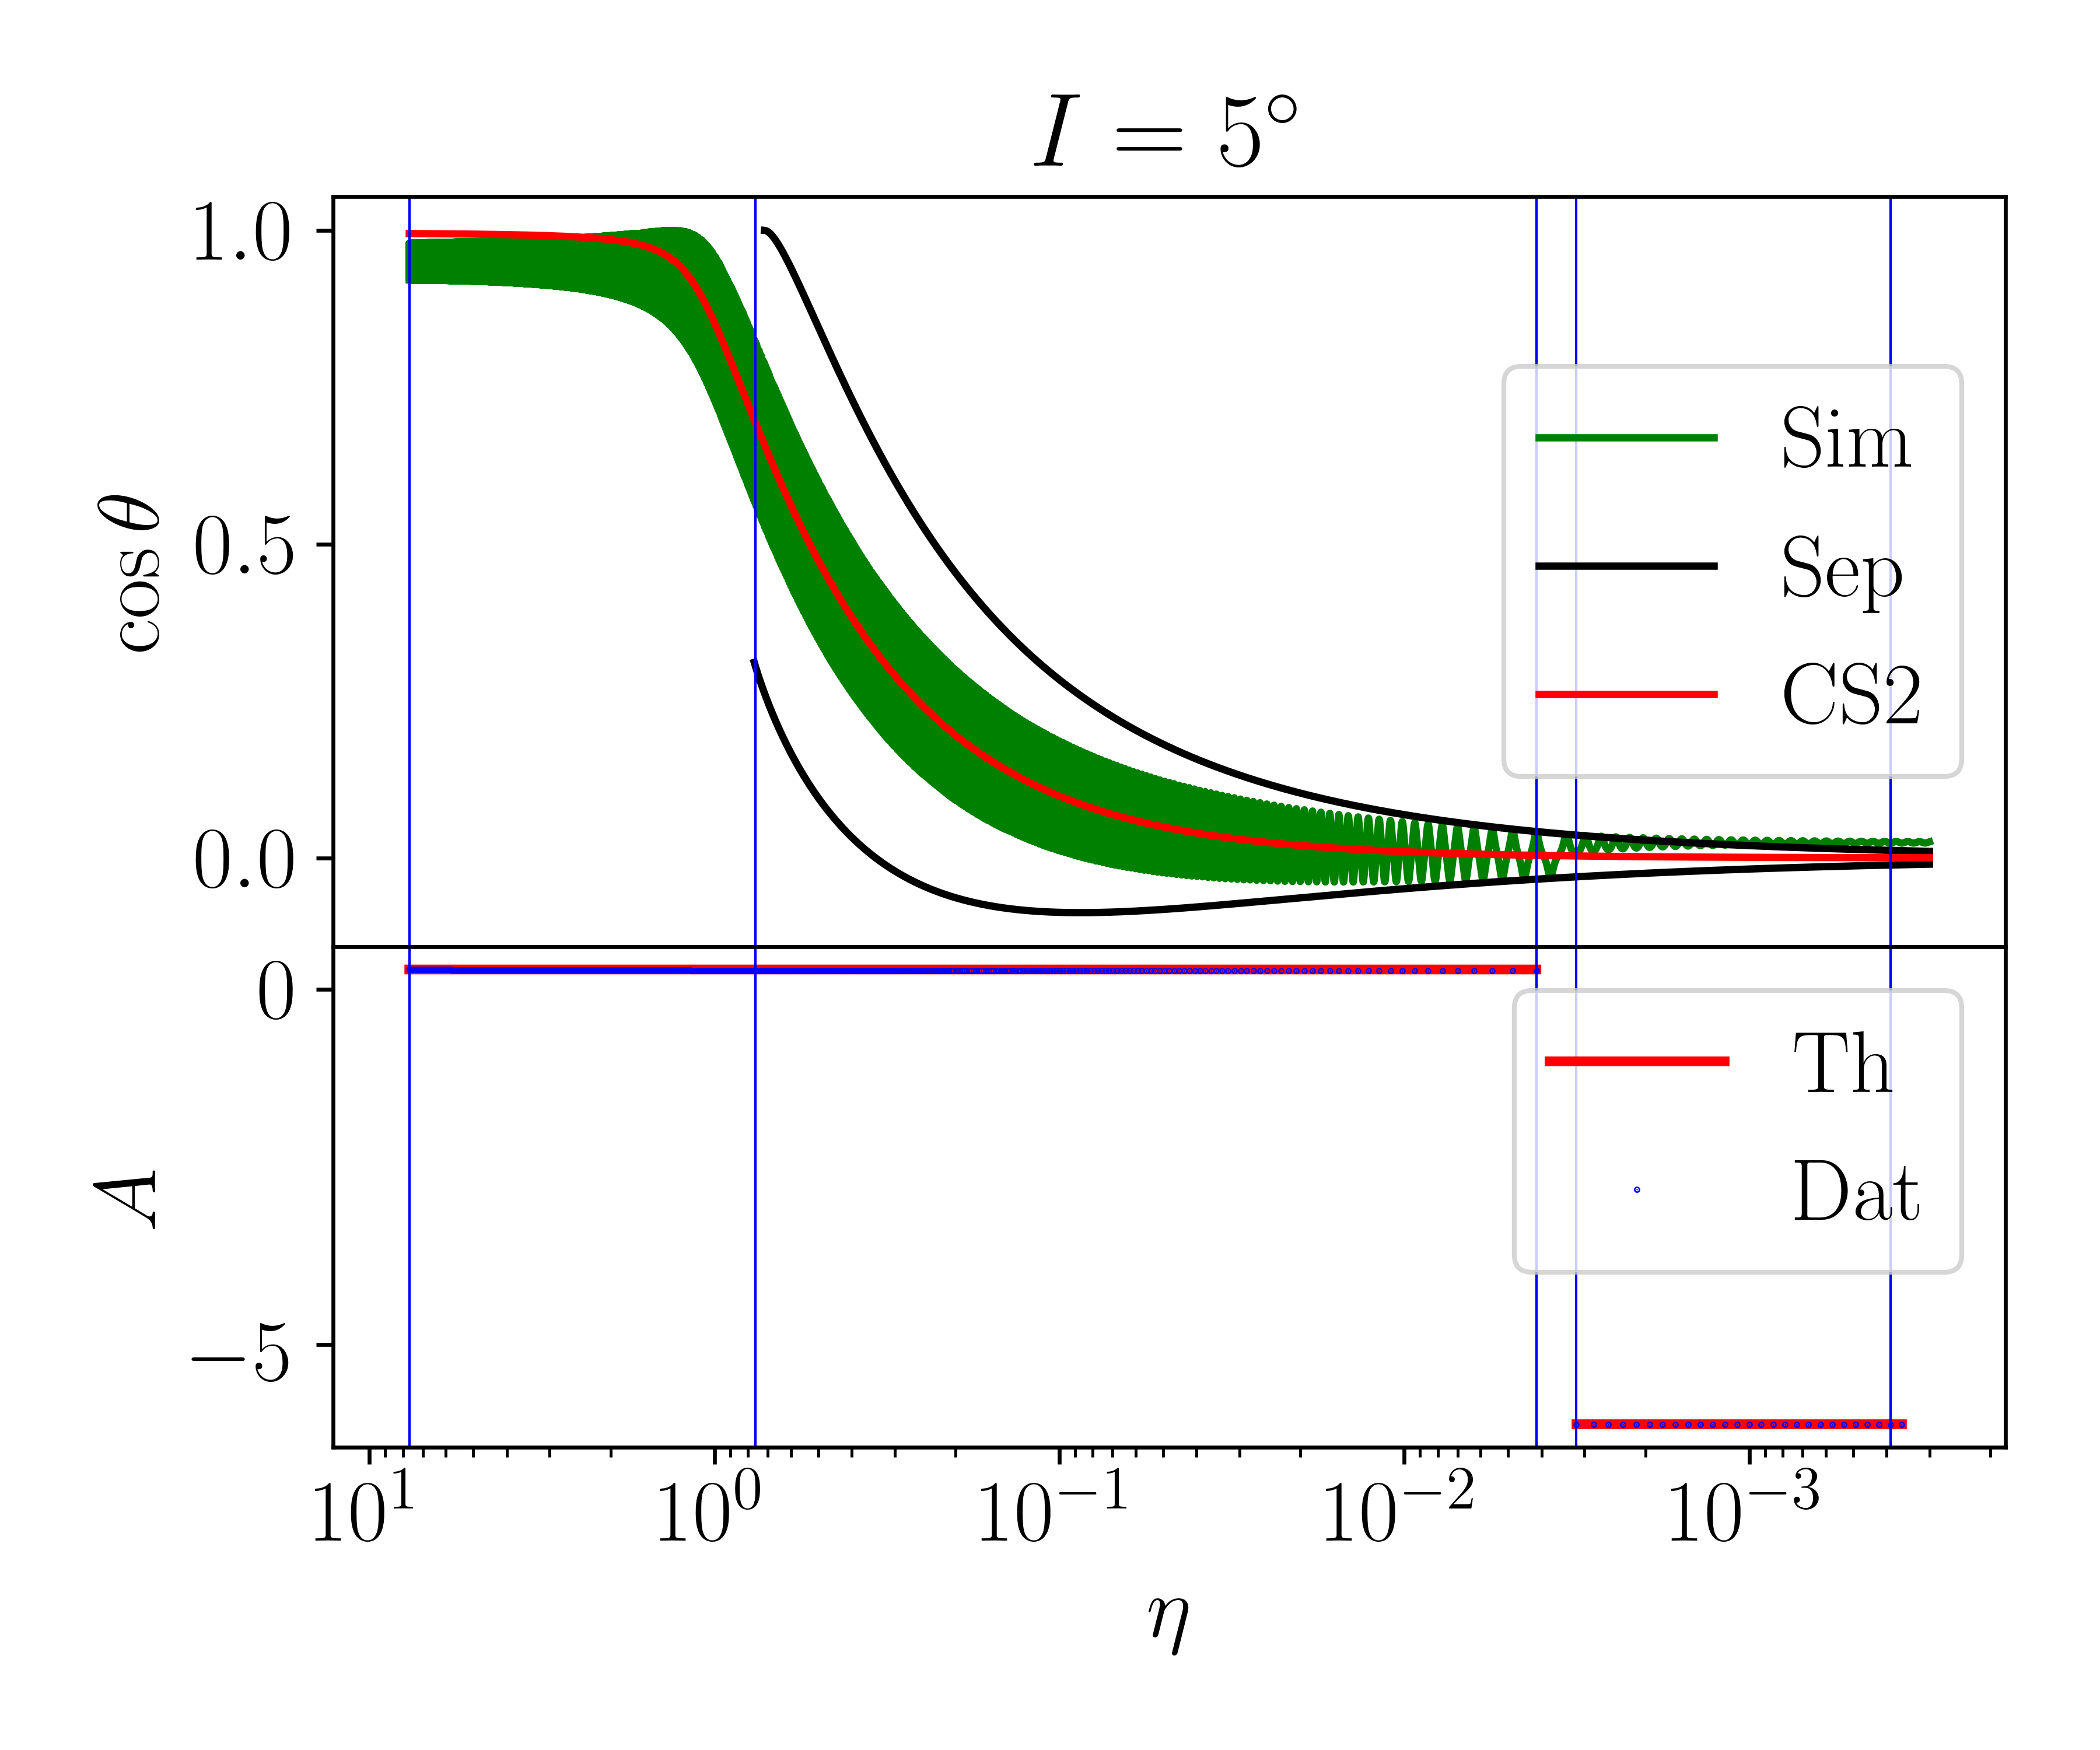
\includegraphics[width=\columnwidth]{../initial/2_toy2/3testo21.png}
    \end{subfigure}
    \begin{subfigure}{\columnwidth}
        \centering
        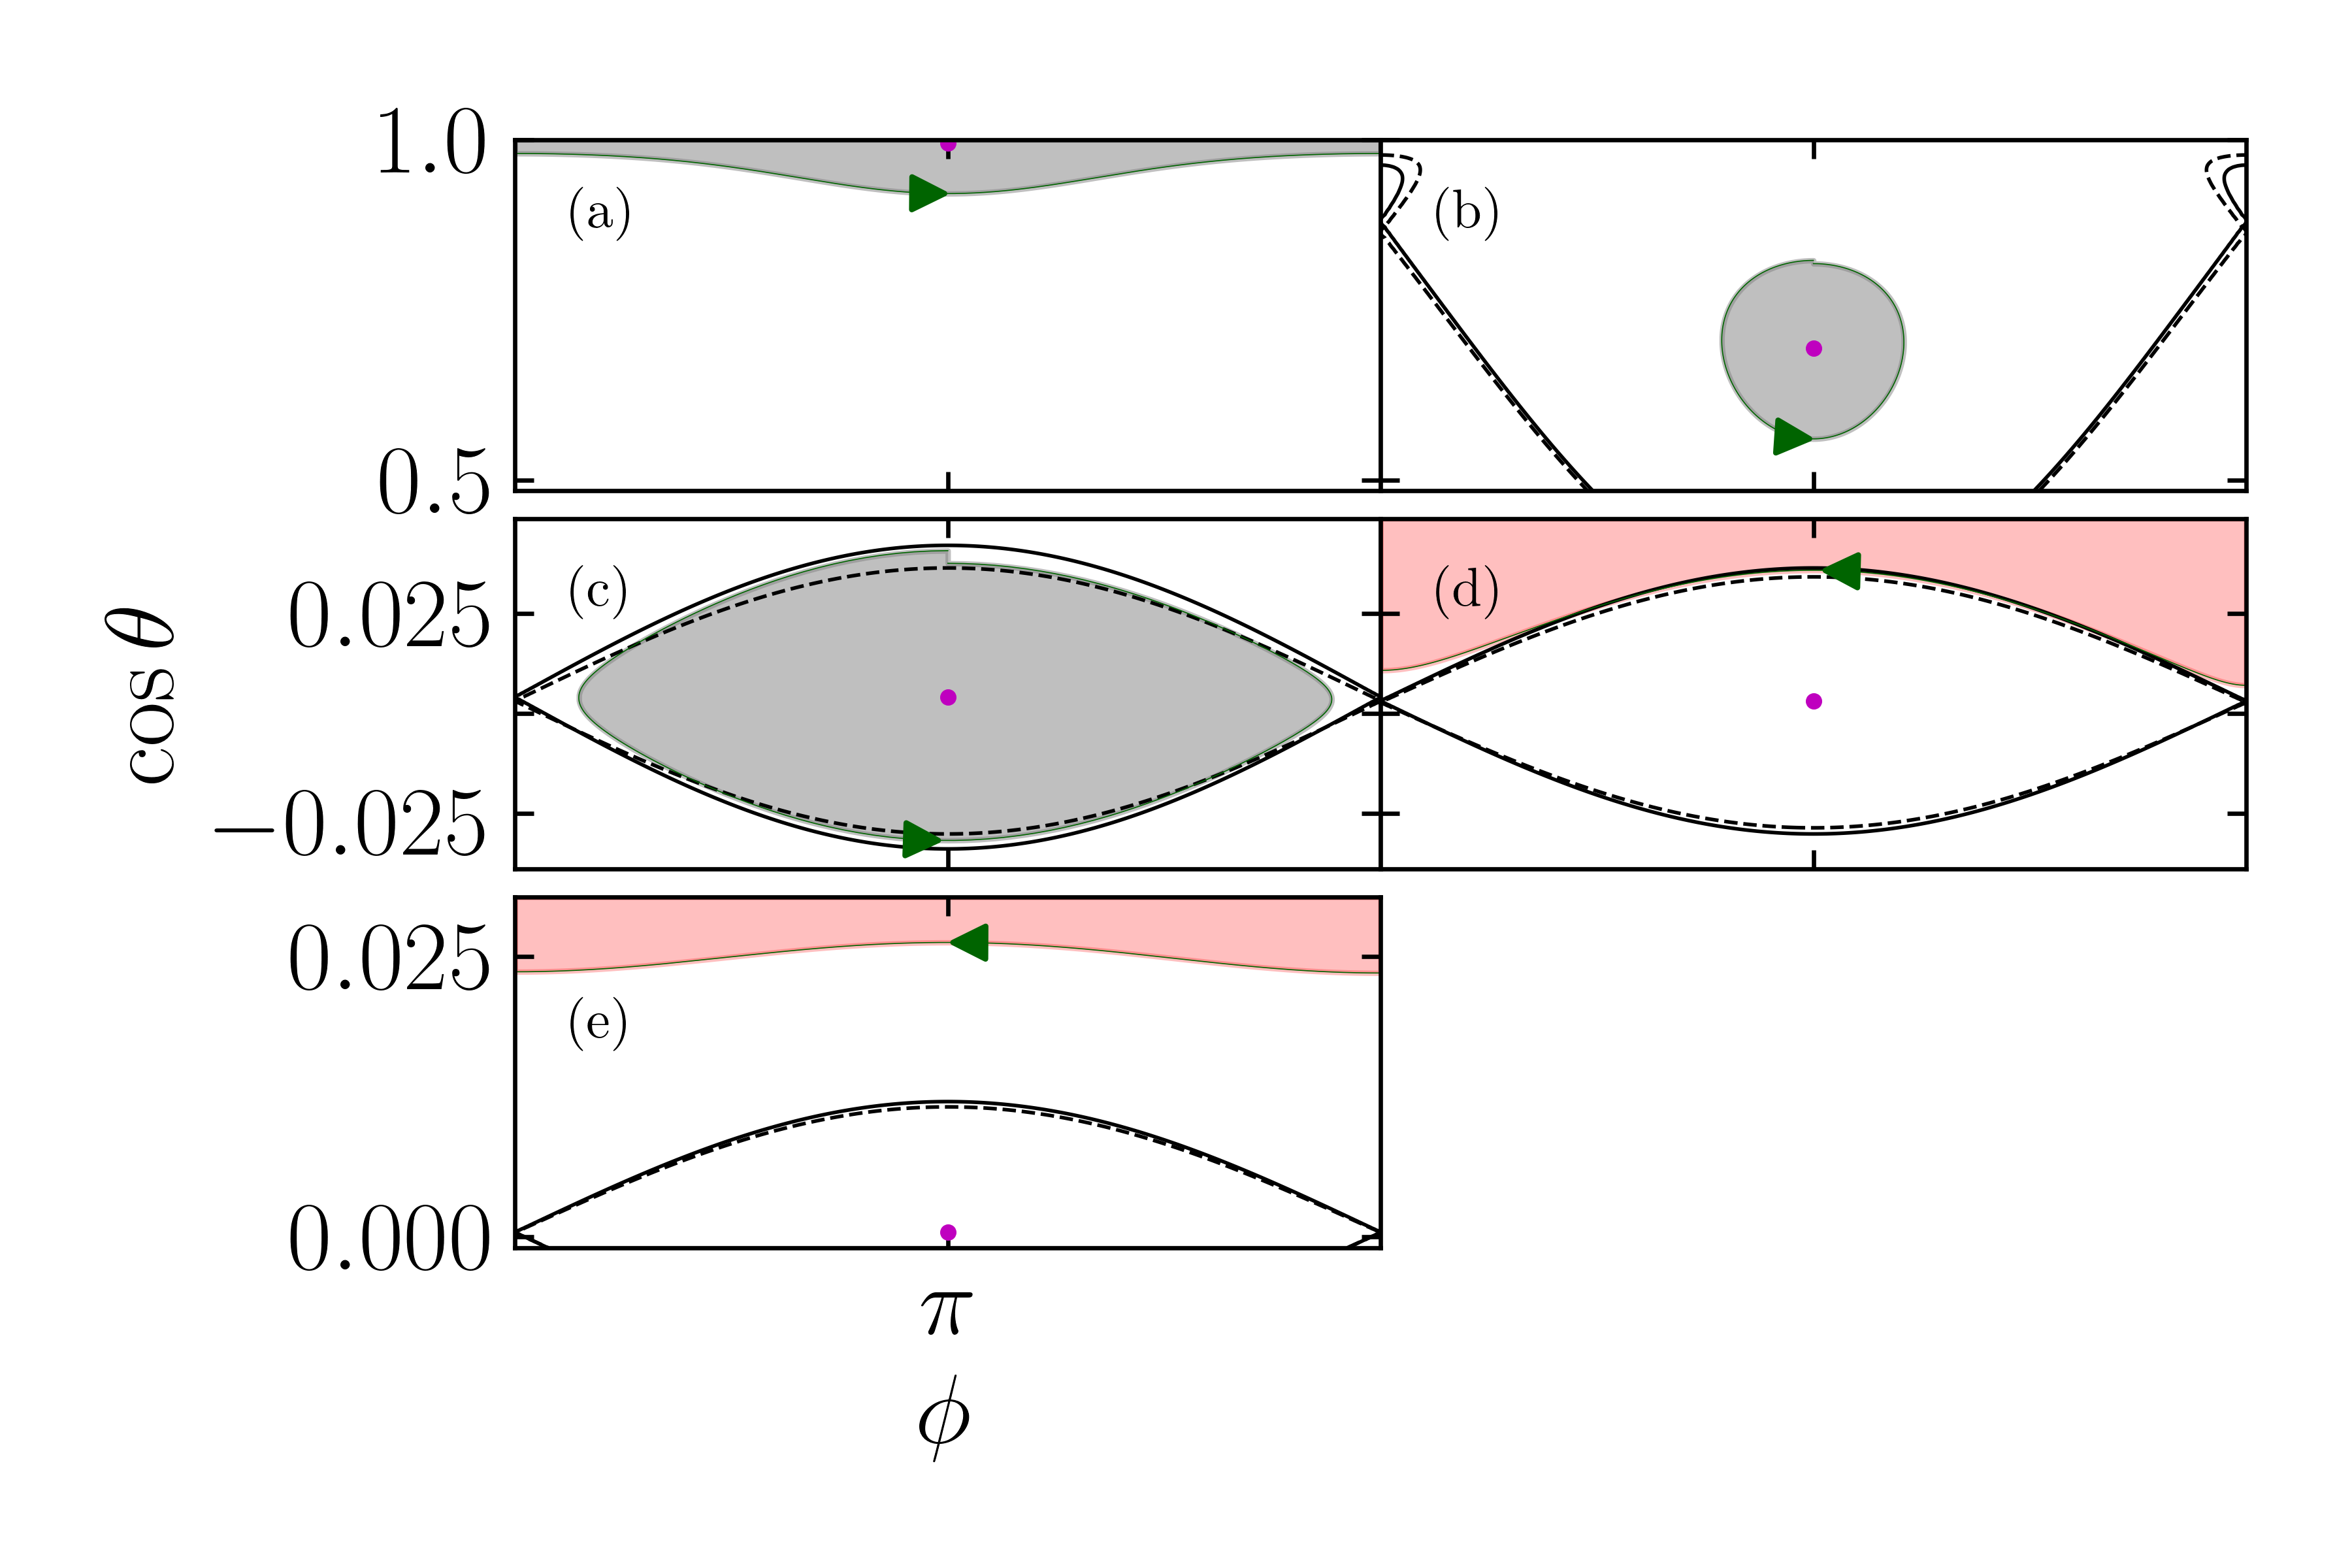
\includegraphics[width=\columnwidth]{../initial/2_toy2/3testo21_subplots.png}
    \end{subfigure}
    \caption{Fiducial simulation following the $A_{II} \to A_{I}$ transition. An
    initial $\theta_{sd, i} = 0.3\;\mathrm{rad} \approx 17.2^\circ$ was used, as
    well as $\epsilon = 3 \times 10^{-4}$. Top plot upper panel: plot of $\cos
    \theta(t)$ (gold) in an example simulation. Overlaid are the locations of
    Cassini State 2 (magenta), and upper and lower bounds on the separatrix
    (black). Note that the trajectory successfully tracks CS2 to a misalignment
    angle $\theta \approx 90^\circ$. Vertical green lines denote times portrayed
    in bottom plot. Top plot lower panel: plot of the enclosed separatrix area
    obtained by integrating the simulated trajectory (blue dots) and adiabatic
    theory (red line). Lower plot: snapshots in the $\p{\cos \theta, \phi}$
    space of the simulation trajectories for the times demarcated in green
    above, corresponding to the start of the simulation, the appearance of the
    separatrix, two panels depicting the separatrix crossing process, and a
    final snapshot at $\eta = 10^{-3.5}$. Gold dots denote a full circulation or
    libration cycle at the selected time, while the separatrix at the start/end
    of the portrayed cycle are shown in solid/dashed black lines respectively.
    Also labeled is CS2 (magenta). Finally, the enclosed phase space area is
    shaded in grey ($A > 0$) and red ($A < 0$).}\label{fig:ad_21}
\end{figure}
\begin{figure}
    \centering
    \begin{subfigure}{\columnwidth}
        \centering
        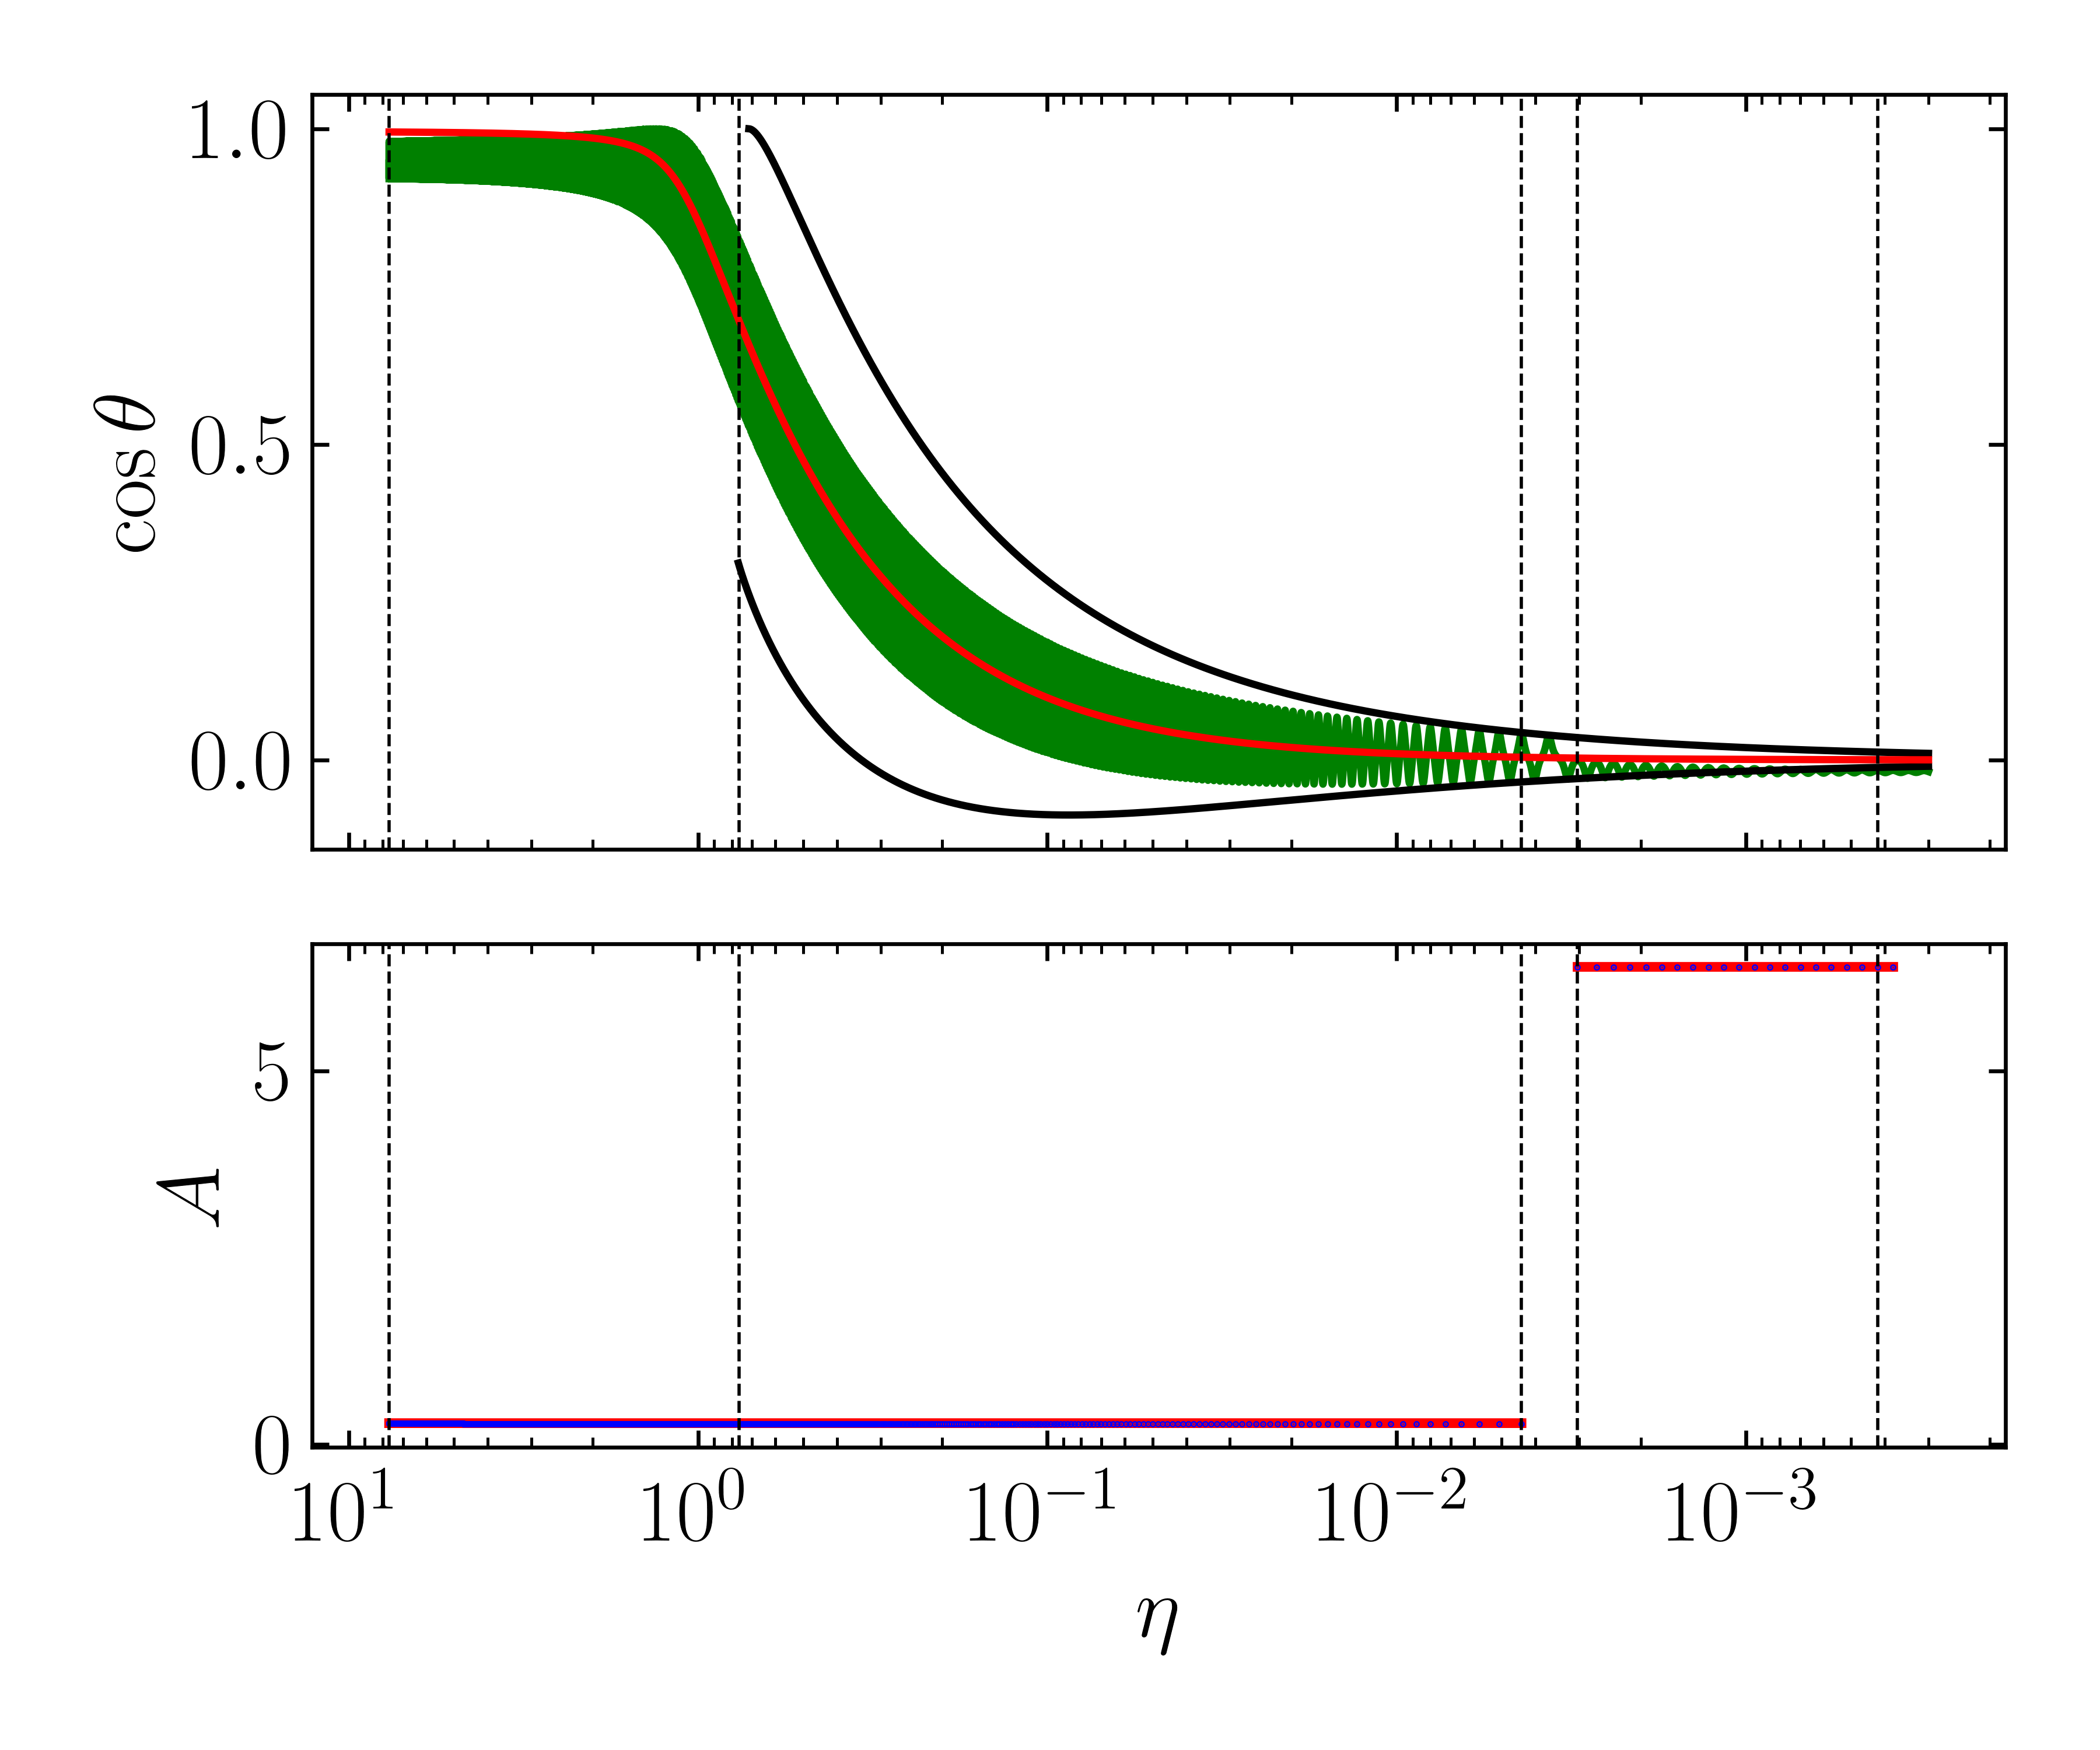
\includegraphics[width=\columnwidth]{../initial/2_toy2/3testo23.png}
    \end{subfigure}
    \begin{subfigure}{\columnwidth}
        \centering
        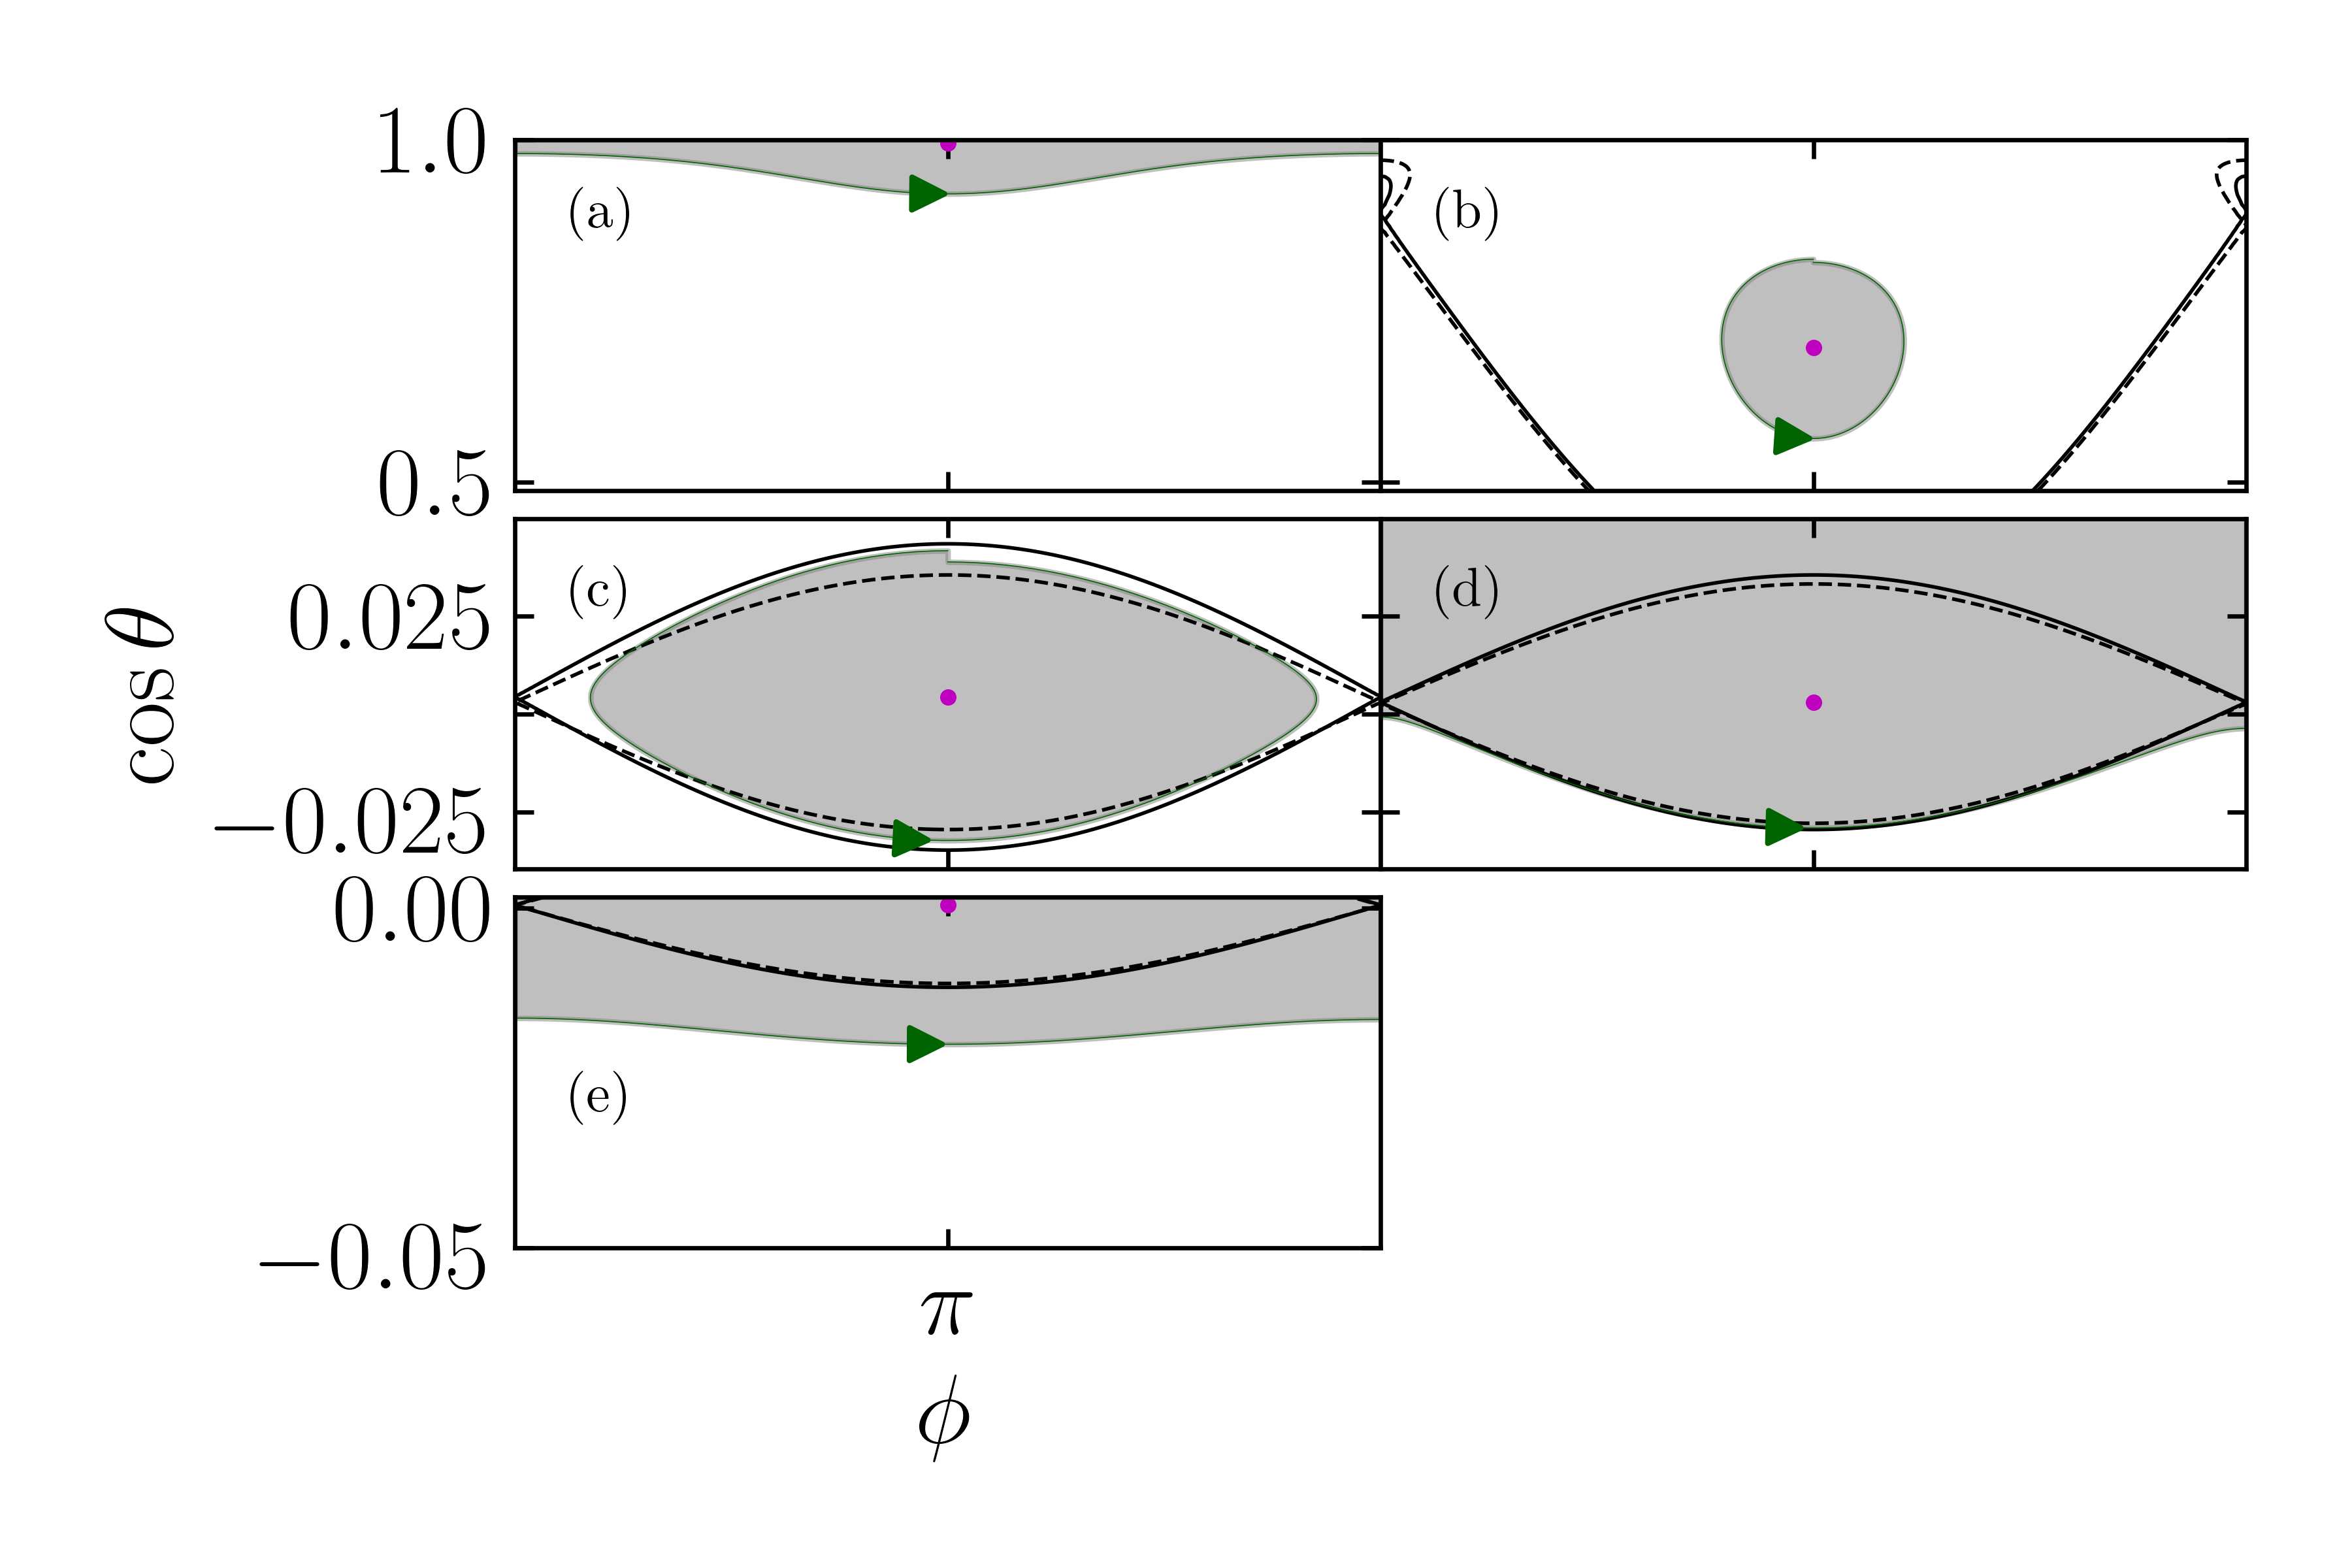
\includegraphics[width=\columnwidth]{../initial/2_toy2/3testo23_subplots.png}
    \end{subfigure}
    \caption{Same as \autoref{fig:ad_21} but for the $A_2 \to A_3$ track.
    $\theta_{sd, i} = 0.3\;\mathrm{rad} \approx 17.2^\circ$, and $\epsilon =
    3.01 \times 10^{-4}$.}\label{fig:ad_23}
\end{figure}
\begin{figure}
    \centering
    \begin{subfigure}{\columnwidth}
        \centering
        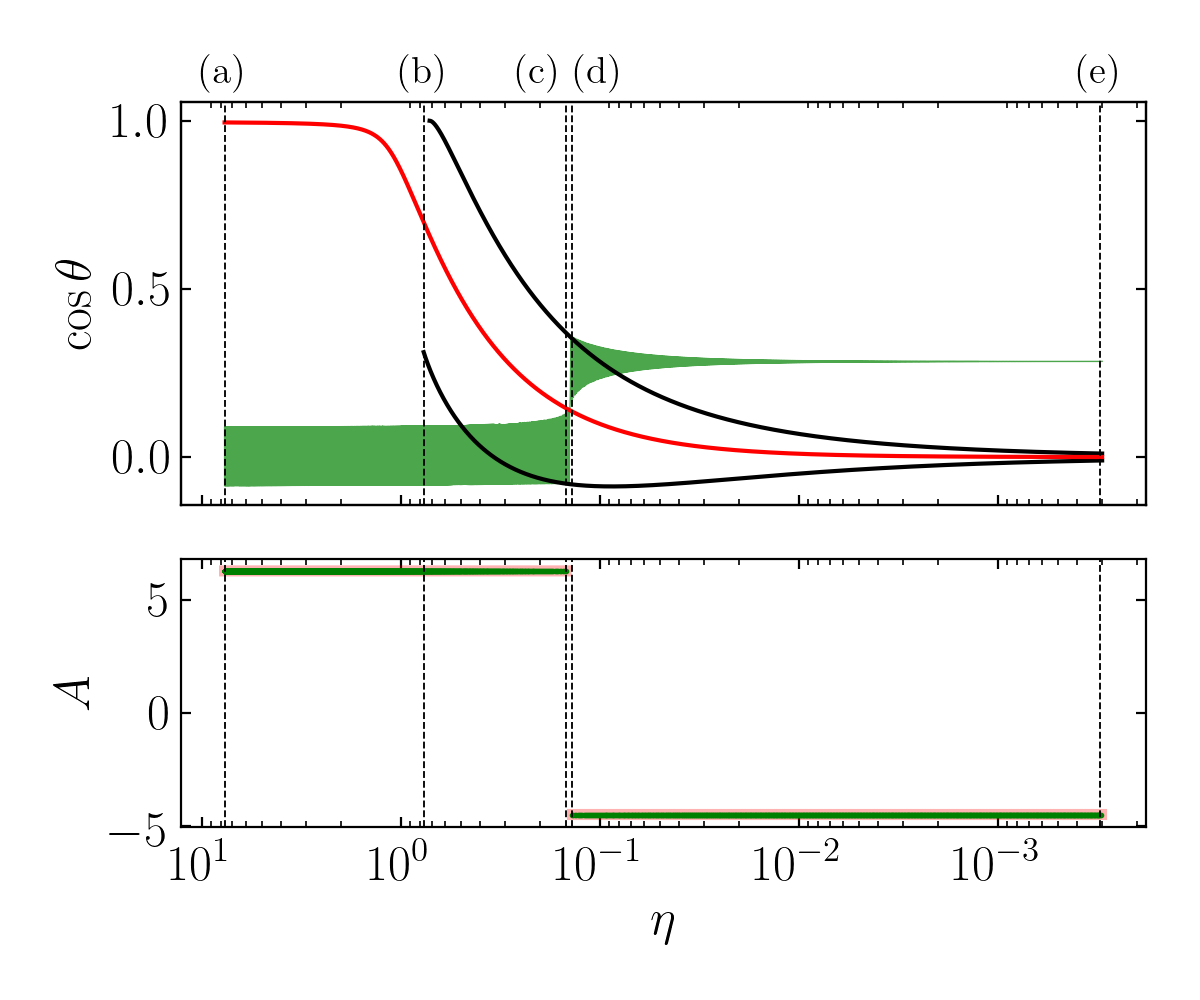
\includegraphics[width=\columnwidth]{../initial/2_toy2/3testo31.png}
    \end{subfigure}
    \begin{subfigure}{\columnwidth}
        \centering
        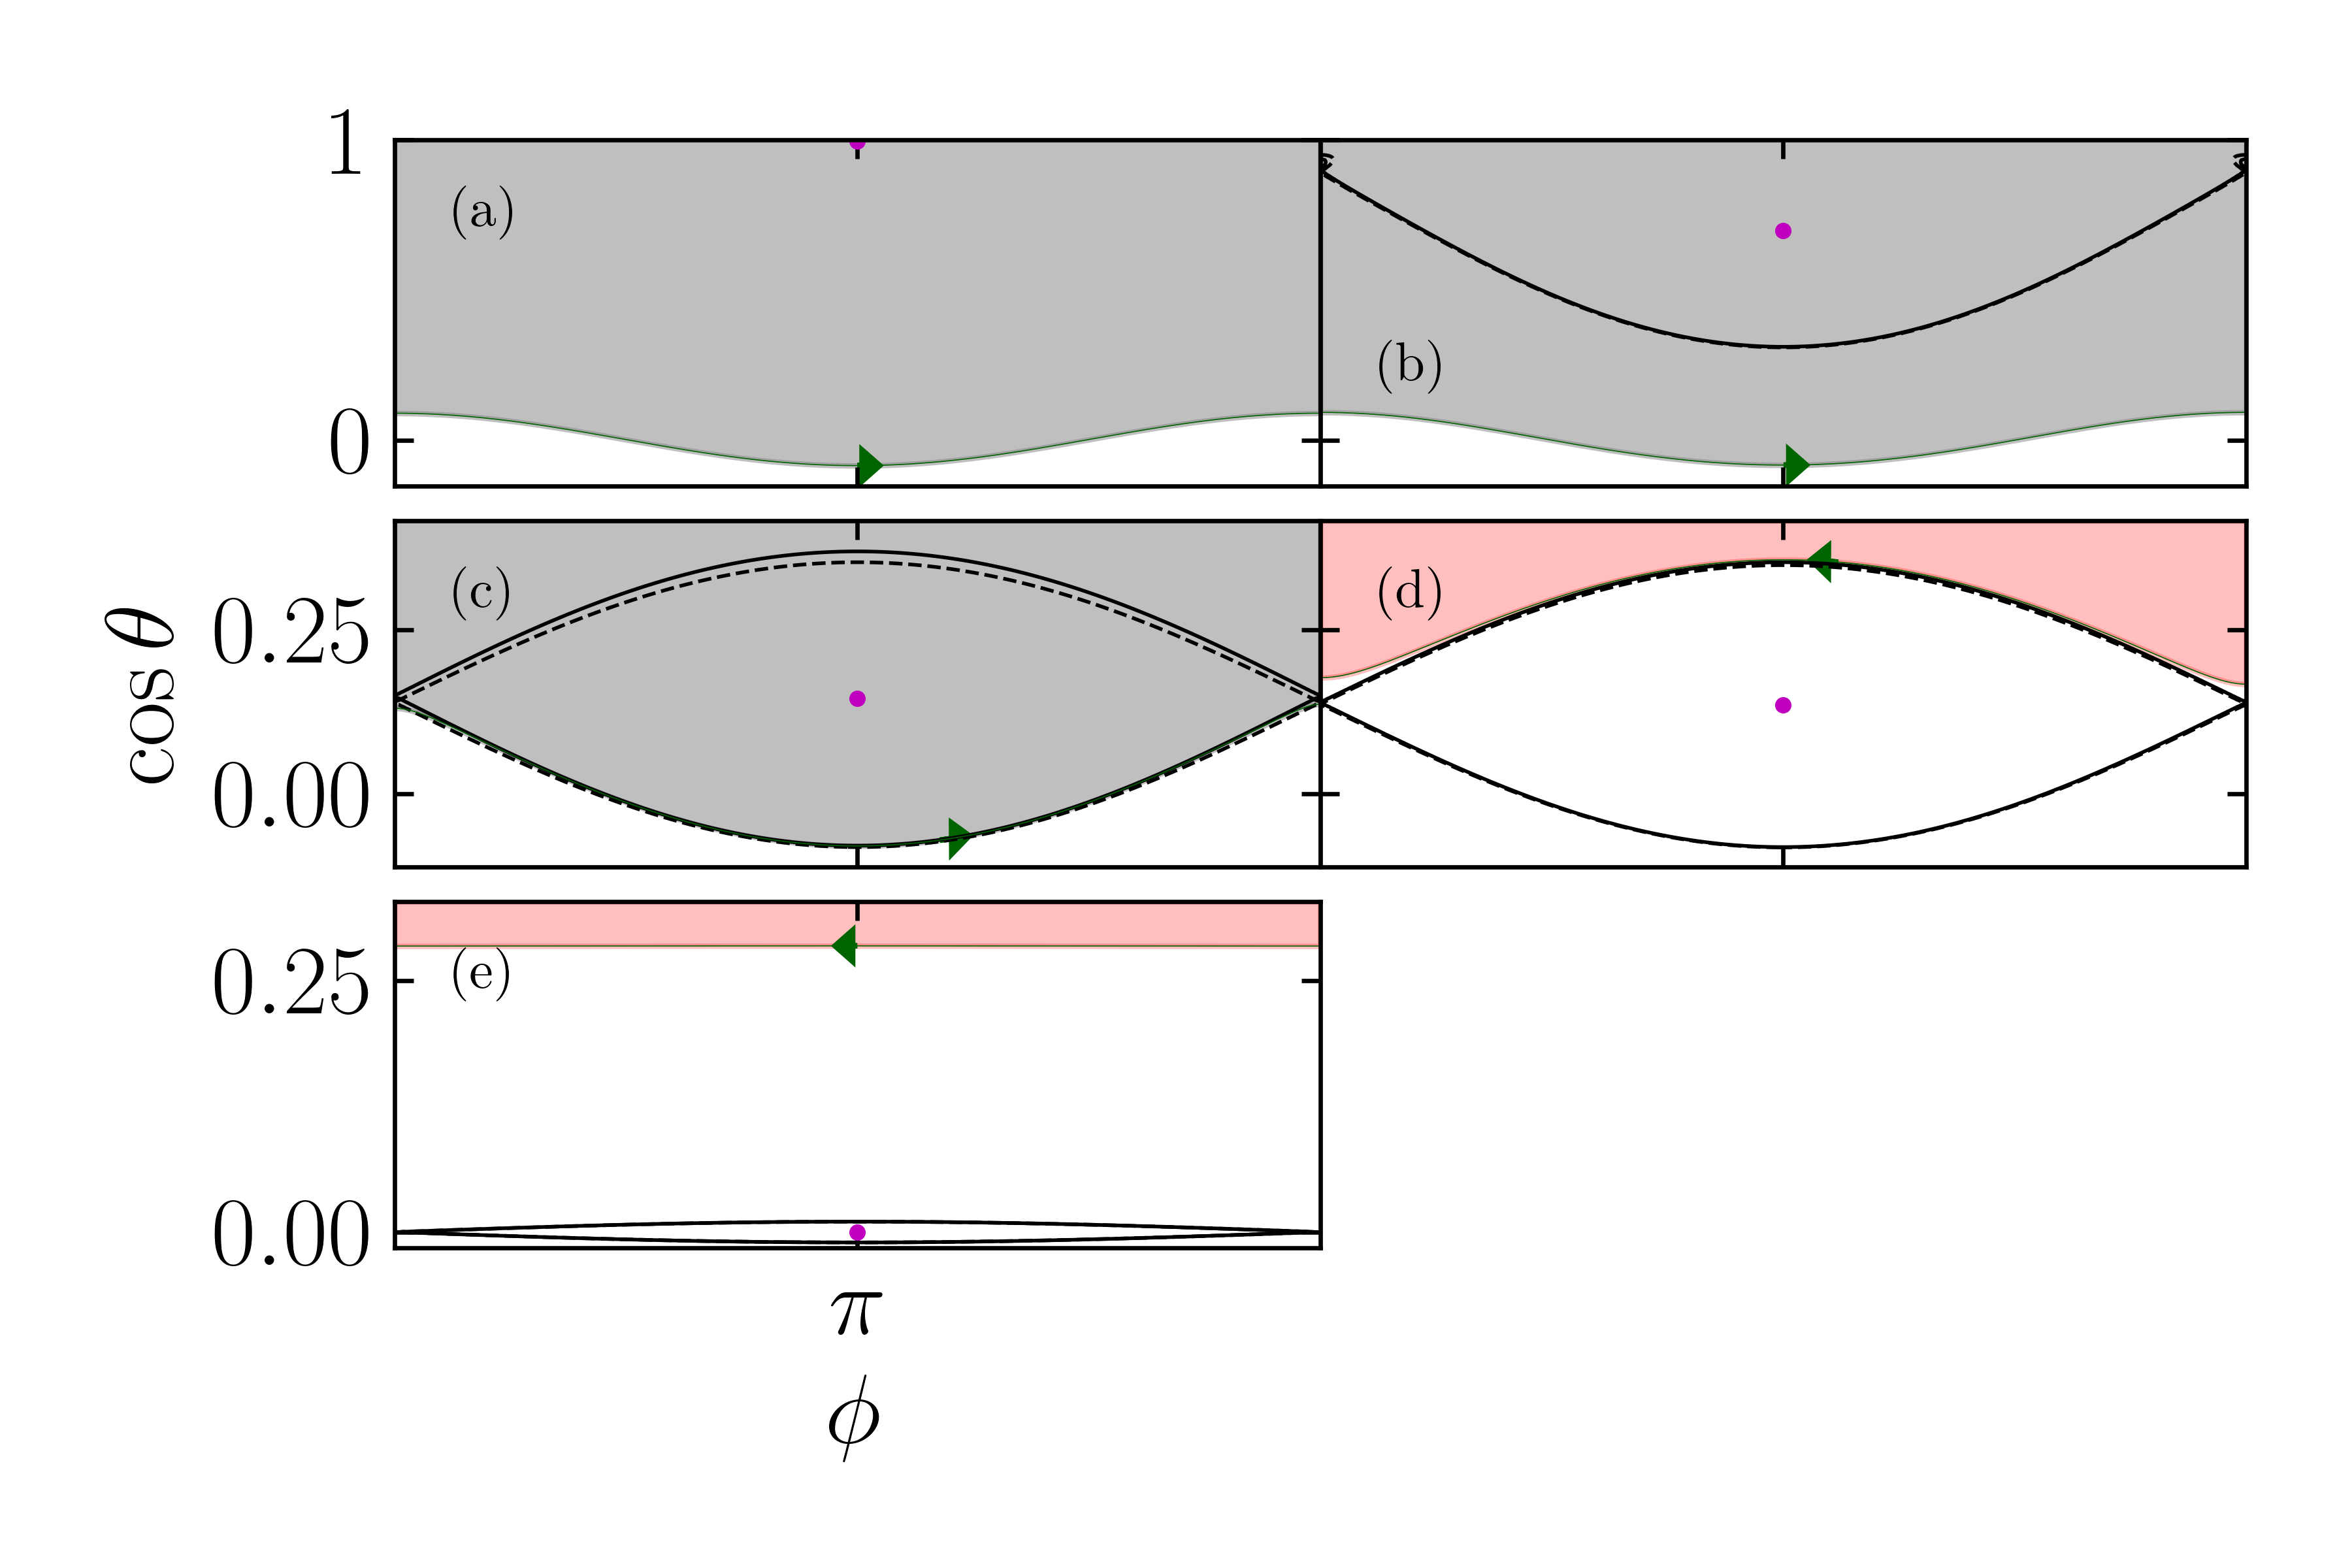
\includegraphics[width=\columnwidth]{../initial/2_toy2/3testo31_subplots.png}
    \end{subfigure}
    \caption{Same as \autoref{fig:ad_21} but for the $A_{III} \to A_I$
    track. $\theta_{sd, i} = 89.1^\circ$, and $\epsilon = 3.01 \times
    10^{-4}$.}\label{fig:ad_31}
\end{figure}
\begin{figure}
    \centering
    \begin{subfigure}{\columnwidth}
        \centering
        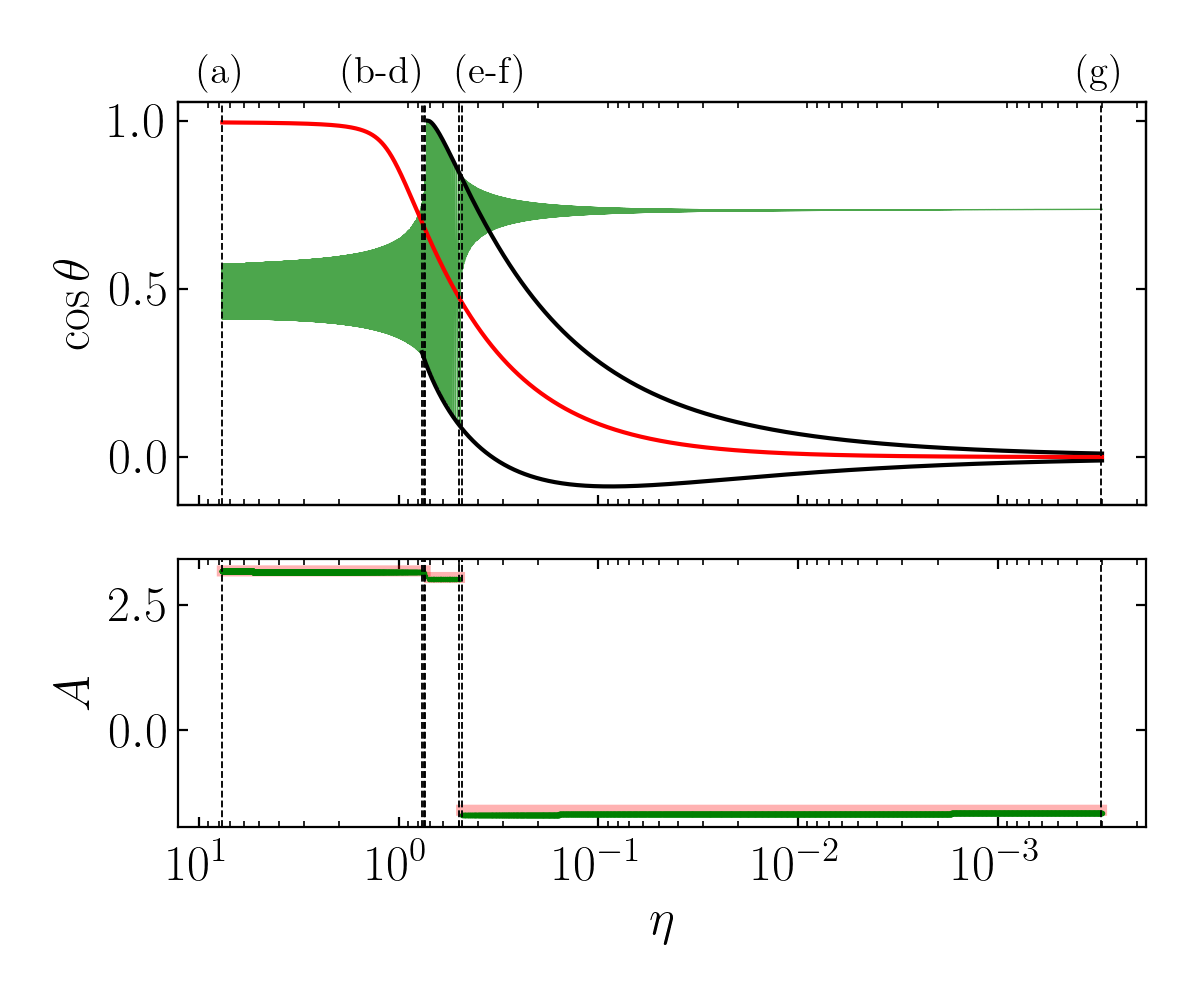
\includegraphics[width=\columnwidth]{../initial/2_toy2/3testo321.png}
    \end{subfigure}
    \begin{subfigure}{\columnwidth}
        \centering
        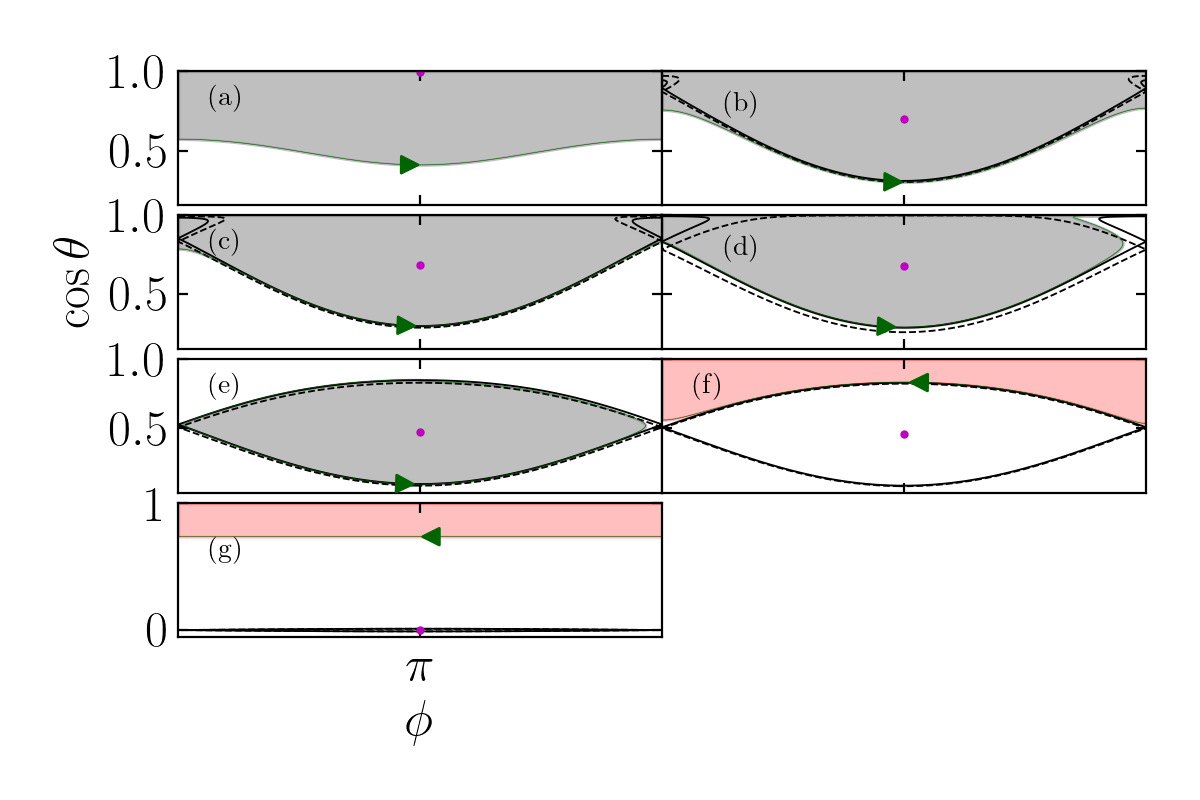
\includegraphics[width=\columnwidth]{../initial/2_toy2/3testo321_subplots.png}
    \end{subfigure}
    \caption{Same as \autoref{fig:ad_21} but for the $A_{III} \to A_{II} \to A_I$
    track. $\theta_{sd, i} = 60^\circ$, and $\epsilon = 3.14 \times 10^{-4}$.
    Two separatrix crossings are shown.}\label{fig:ad_321}
\end{figure}

\subsection{Dynamical Outcomes}\label{ss:ad_ensemble}

Next, we will consider the evolution of a system with arbitrary $\theta_{sd, i}$
starting in the $\eta \gg 1$ regime. By evolving such systems until $\eta \ll
1$, we can measure the final $\theta_f$ values and make comparisons with those
obtained via the dynamical tracks above. Observe that when $\eta \gg 1$,
trajectories librate about $\hat{l}_d$, or equivalently CS2, with approximately
constant $\theta_{sd}$, meaning they enclose phase space area
\begin{equation}
    A_i = 2\pi\p{1 - \cos \theta_{sd, i}}.\label{eq:ai_qsd}
\end{equation}
Thus, for a given $\theta_{sd, i}$, we know immediately which tracks are
accessible and with what probability following the results of
\autoref{ss:zone_transitions}.

We run simulations over a ring of initial conditions at each $\theta_{sd, i}$
and measure the final $\theta_{f}$ values. Since we start with finite $\eta$, we
use the angular distance to CS2 as a proxy for $\theta_{sd, i}$, as it is the
correct quantity to use to make \autoref{eq:ai_qsd} hold exactly. We use
\autoref{eq:ai_qsd} to predict the final obliquities $\theta_f$ according to
each of the dynamical tracks. The agreement of these predictions for $I =
5^\circ, 10^\circ, 20^\circ$ can be seen in \autoref{fig:ad_ensemble},
\autoref{fig:3_ensemble_10_35}, and \autoref{fig:3_ensemble_20_35}.
\begin{figure}
    \centering
    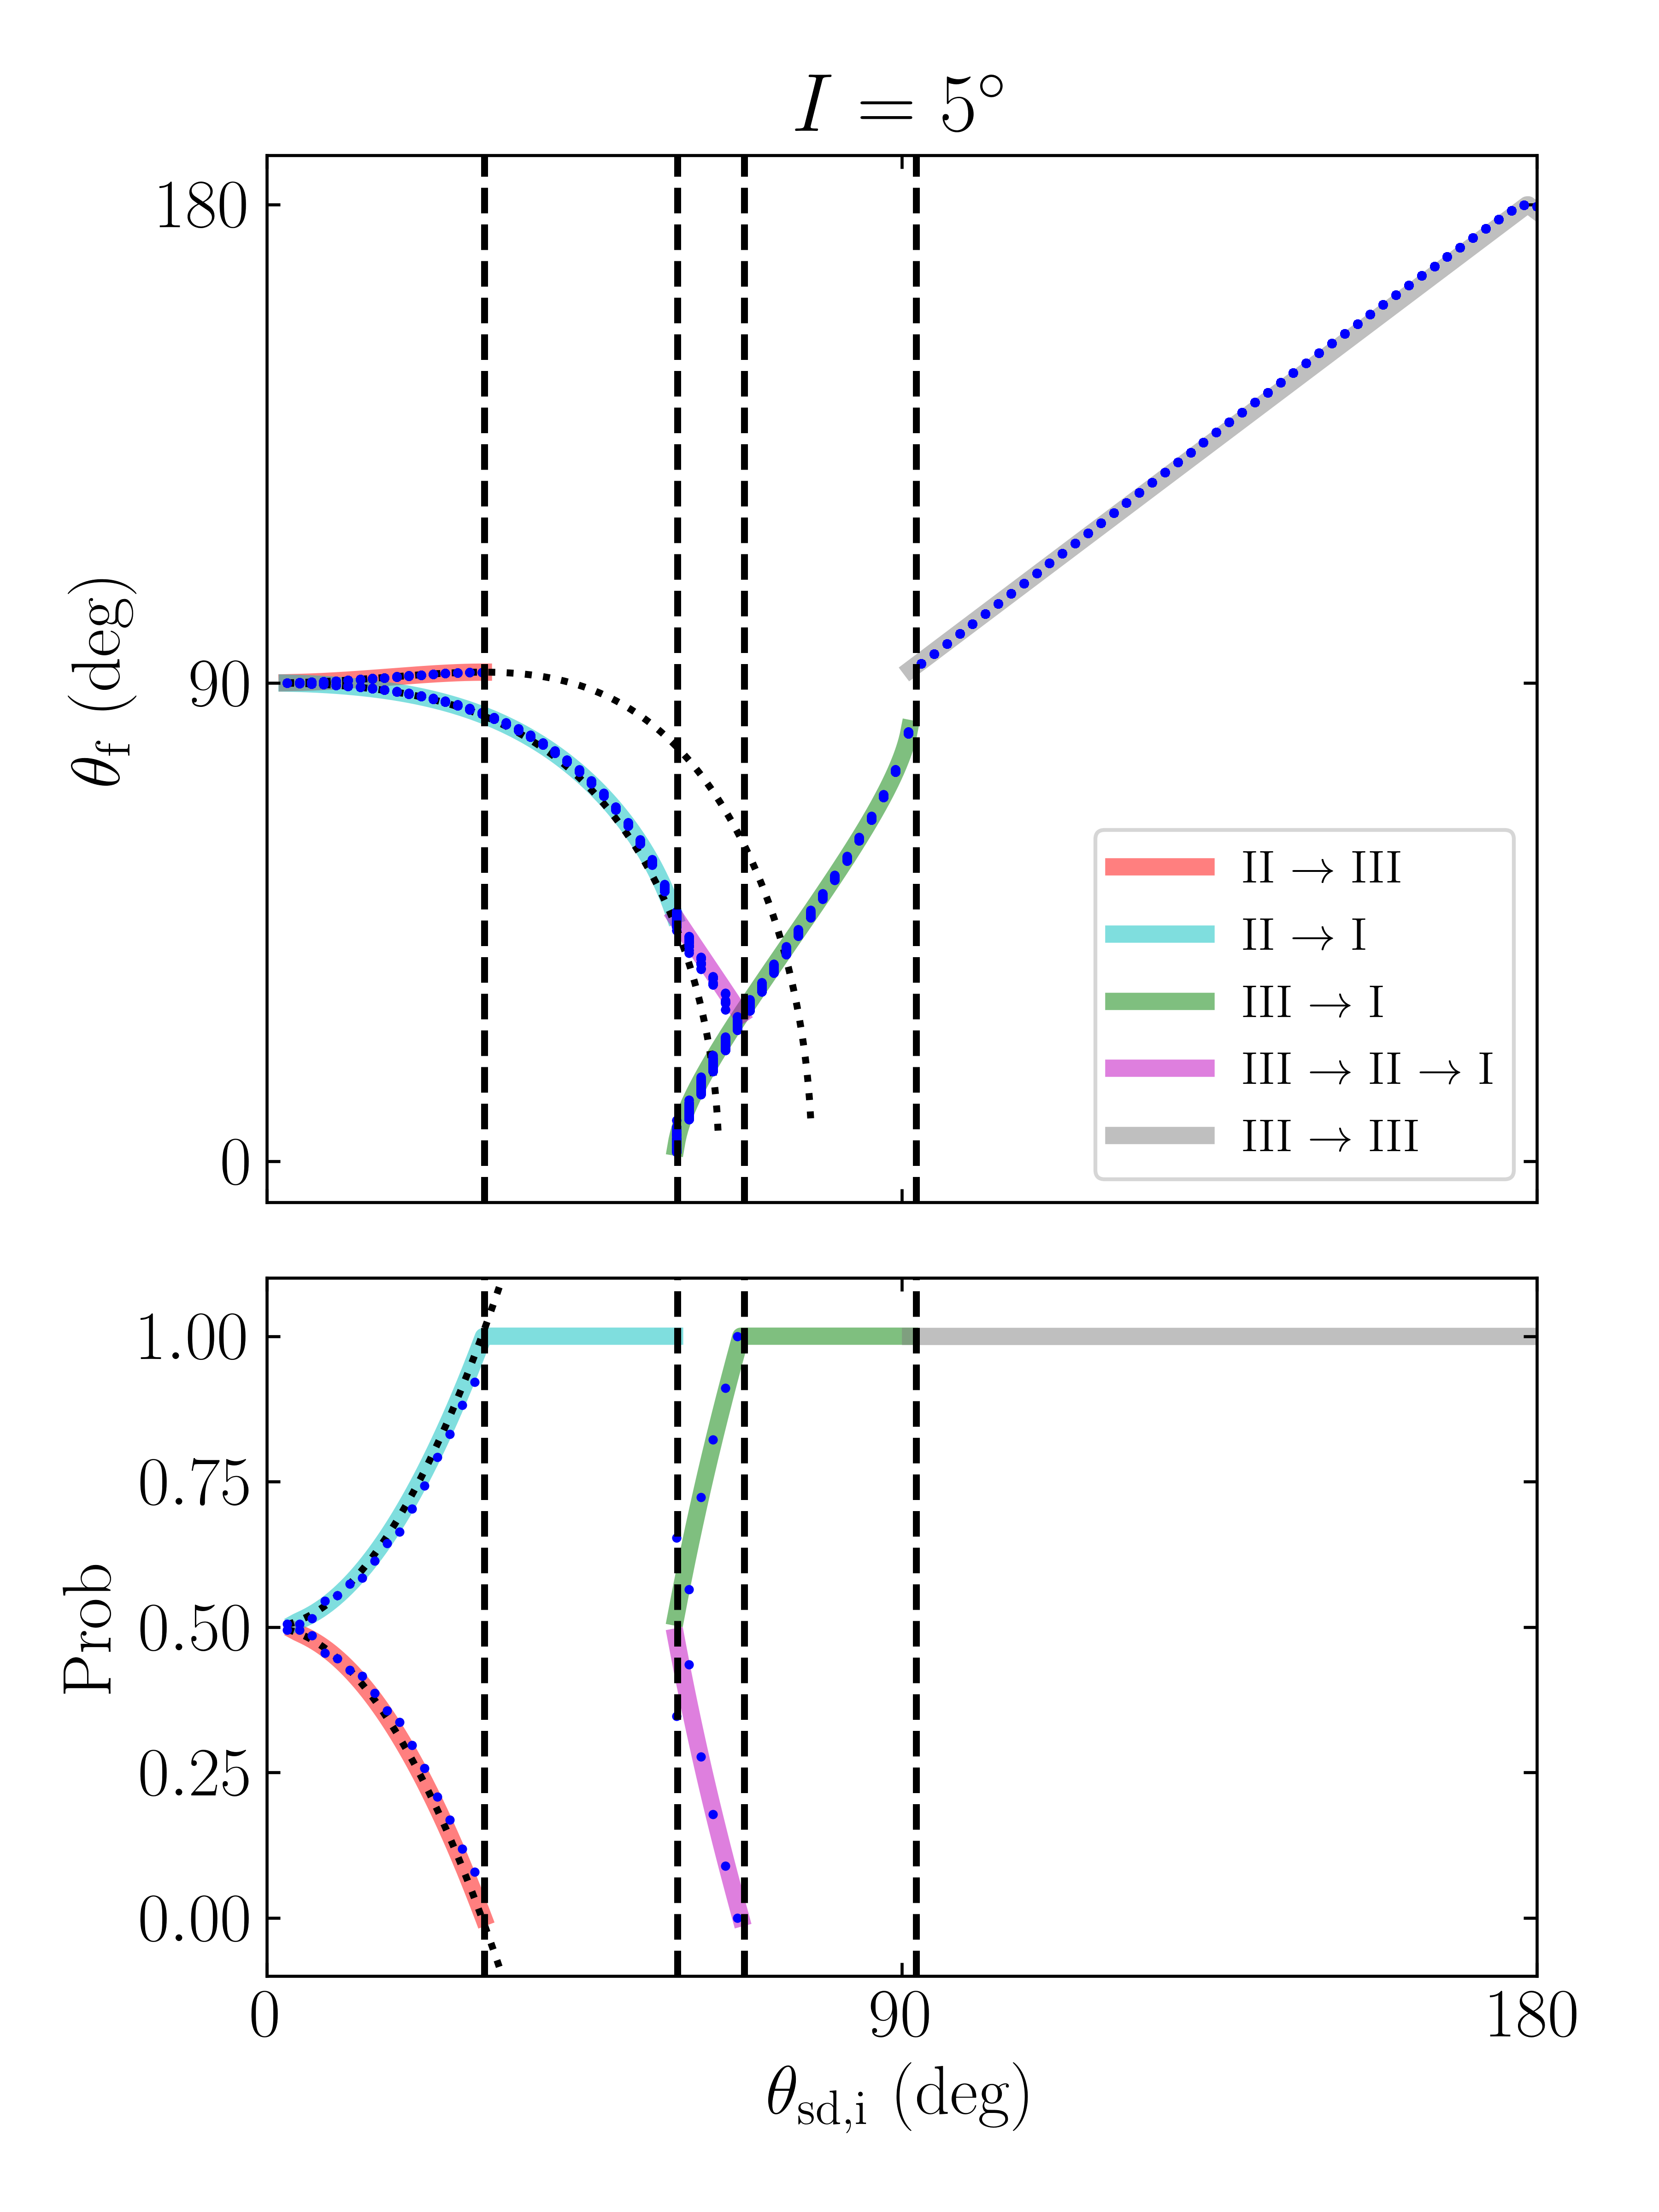
\includegraphics[width=\columnwidth]{../initial/2_toy2/3_ensemble_05_35.png}
    \caption{Top: $\theta_{f}\p{\theta_{sd, i}}$, overlaid with semi-analytic
    predictions of the $\theta_{ f}$ for each of the four nontrivial
    dynamical tracks in colored lines. Bottom: Semi-analytic probabilities of
    each of the dynamical tracks for each $\theta_{sd, i}$. The five regimes of
    $\theta_{sd, i}$ values correspond to the five regimes of $A_i$ discussed in
    \autoref{ss:zone_transitions} when using \autoref{eq:ai_qsd} to relate
    $A_i\p{\theta_{sd, i}}$. }\label{fig:ad_ensemble}
\end{figure}
\begin{figure}
    \centering
    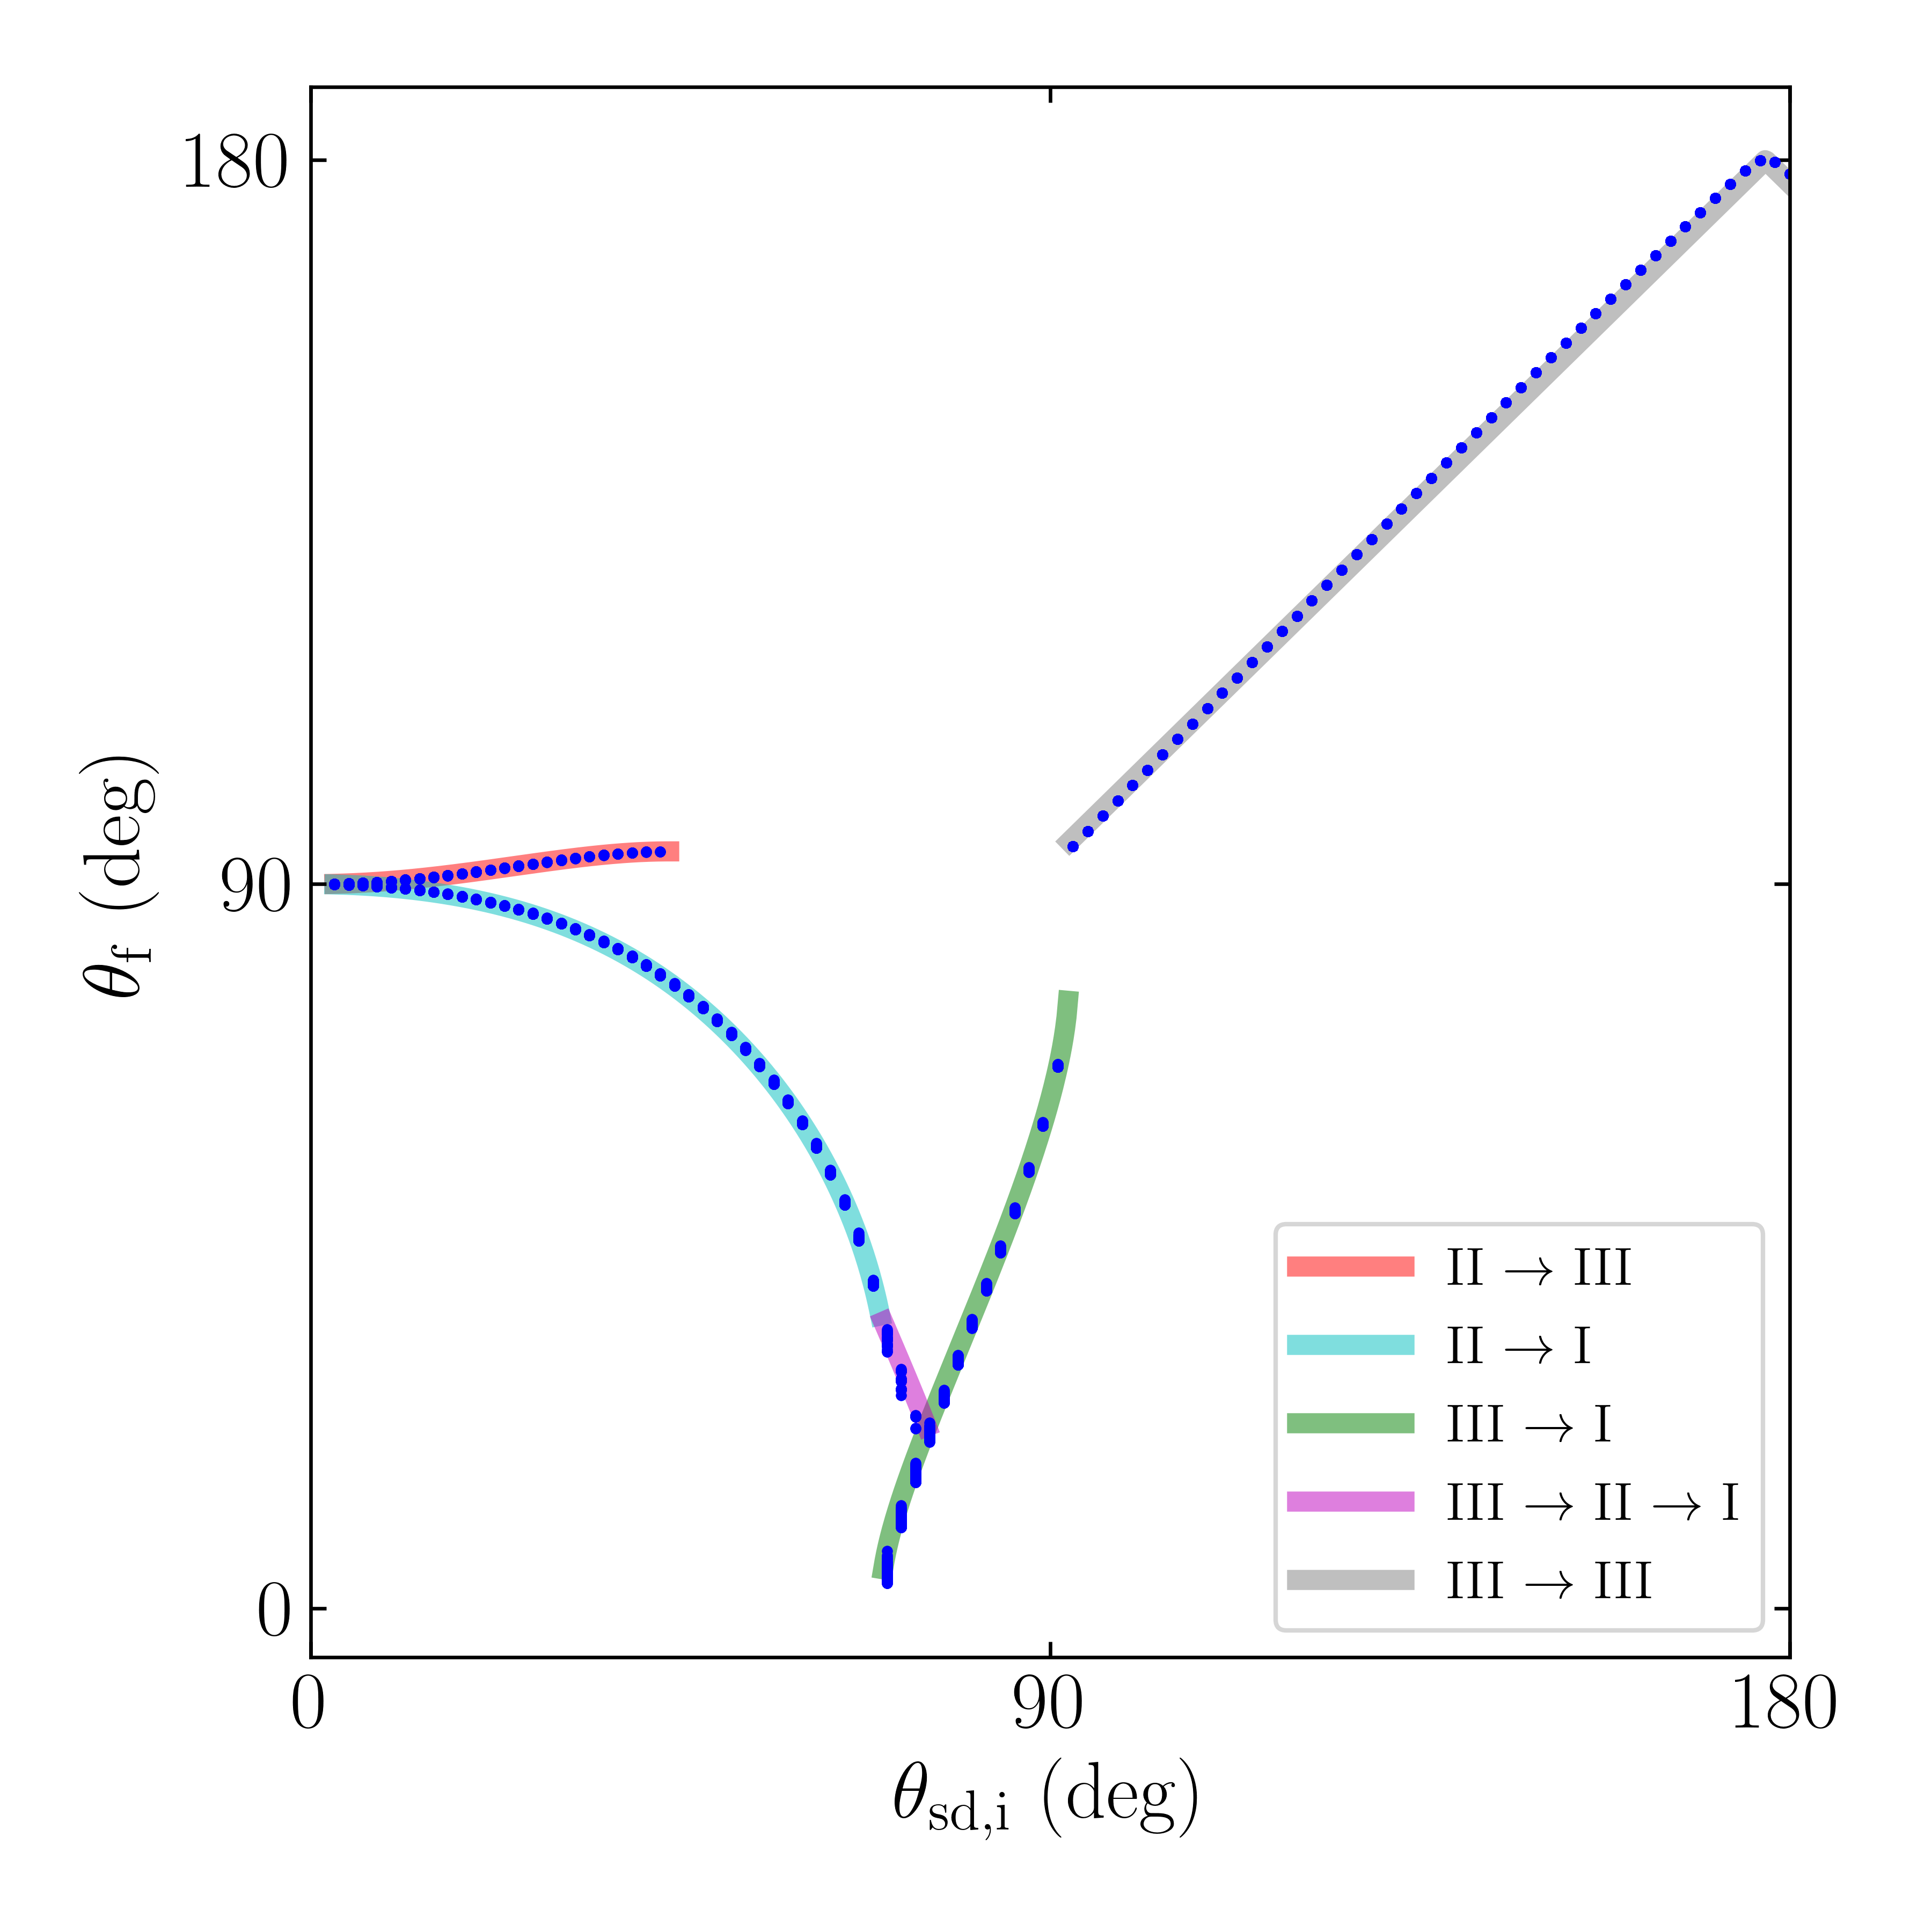
\includegraphics[width=\columnwidth]{../initial/2_toy2/3_ensemble_10_35.png}
    \caption{Same as \autoref{fig:ad_ensemble} but for $I =
    10^\circ$.}\label{fig:3_ensemble_10_35}
\end{figure}
\begin{figure}
    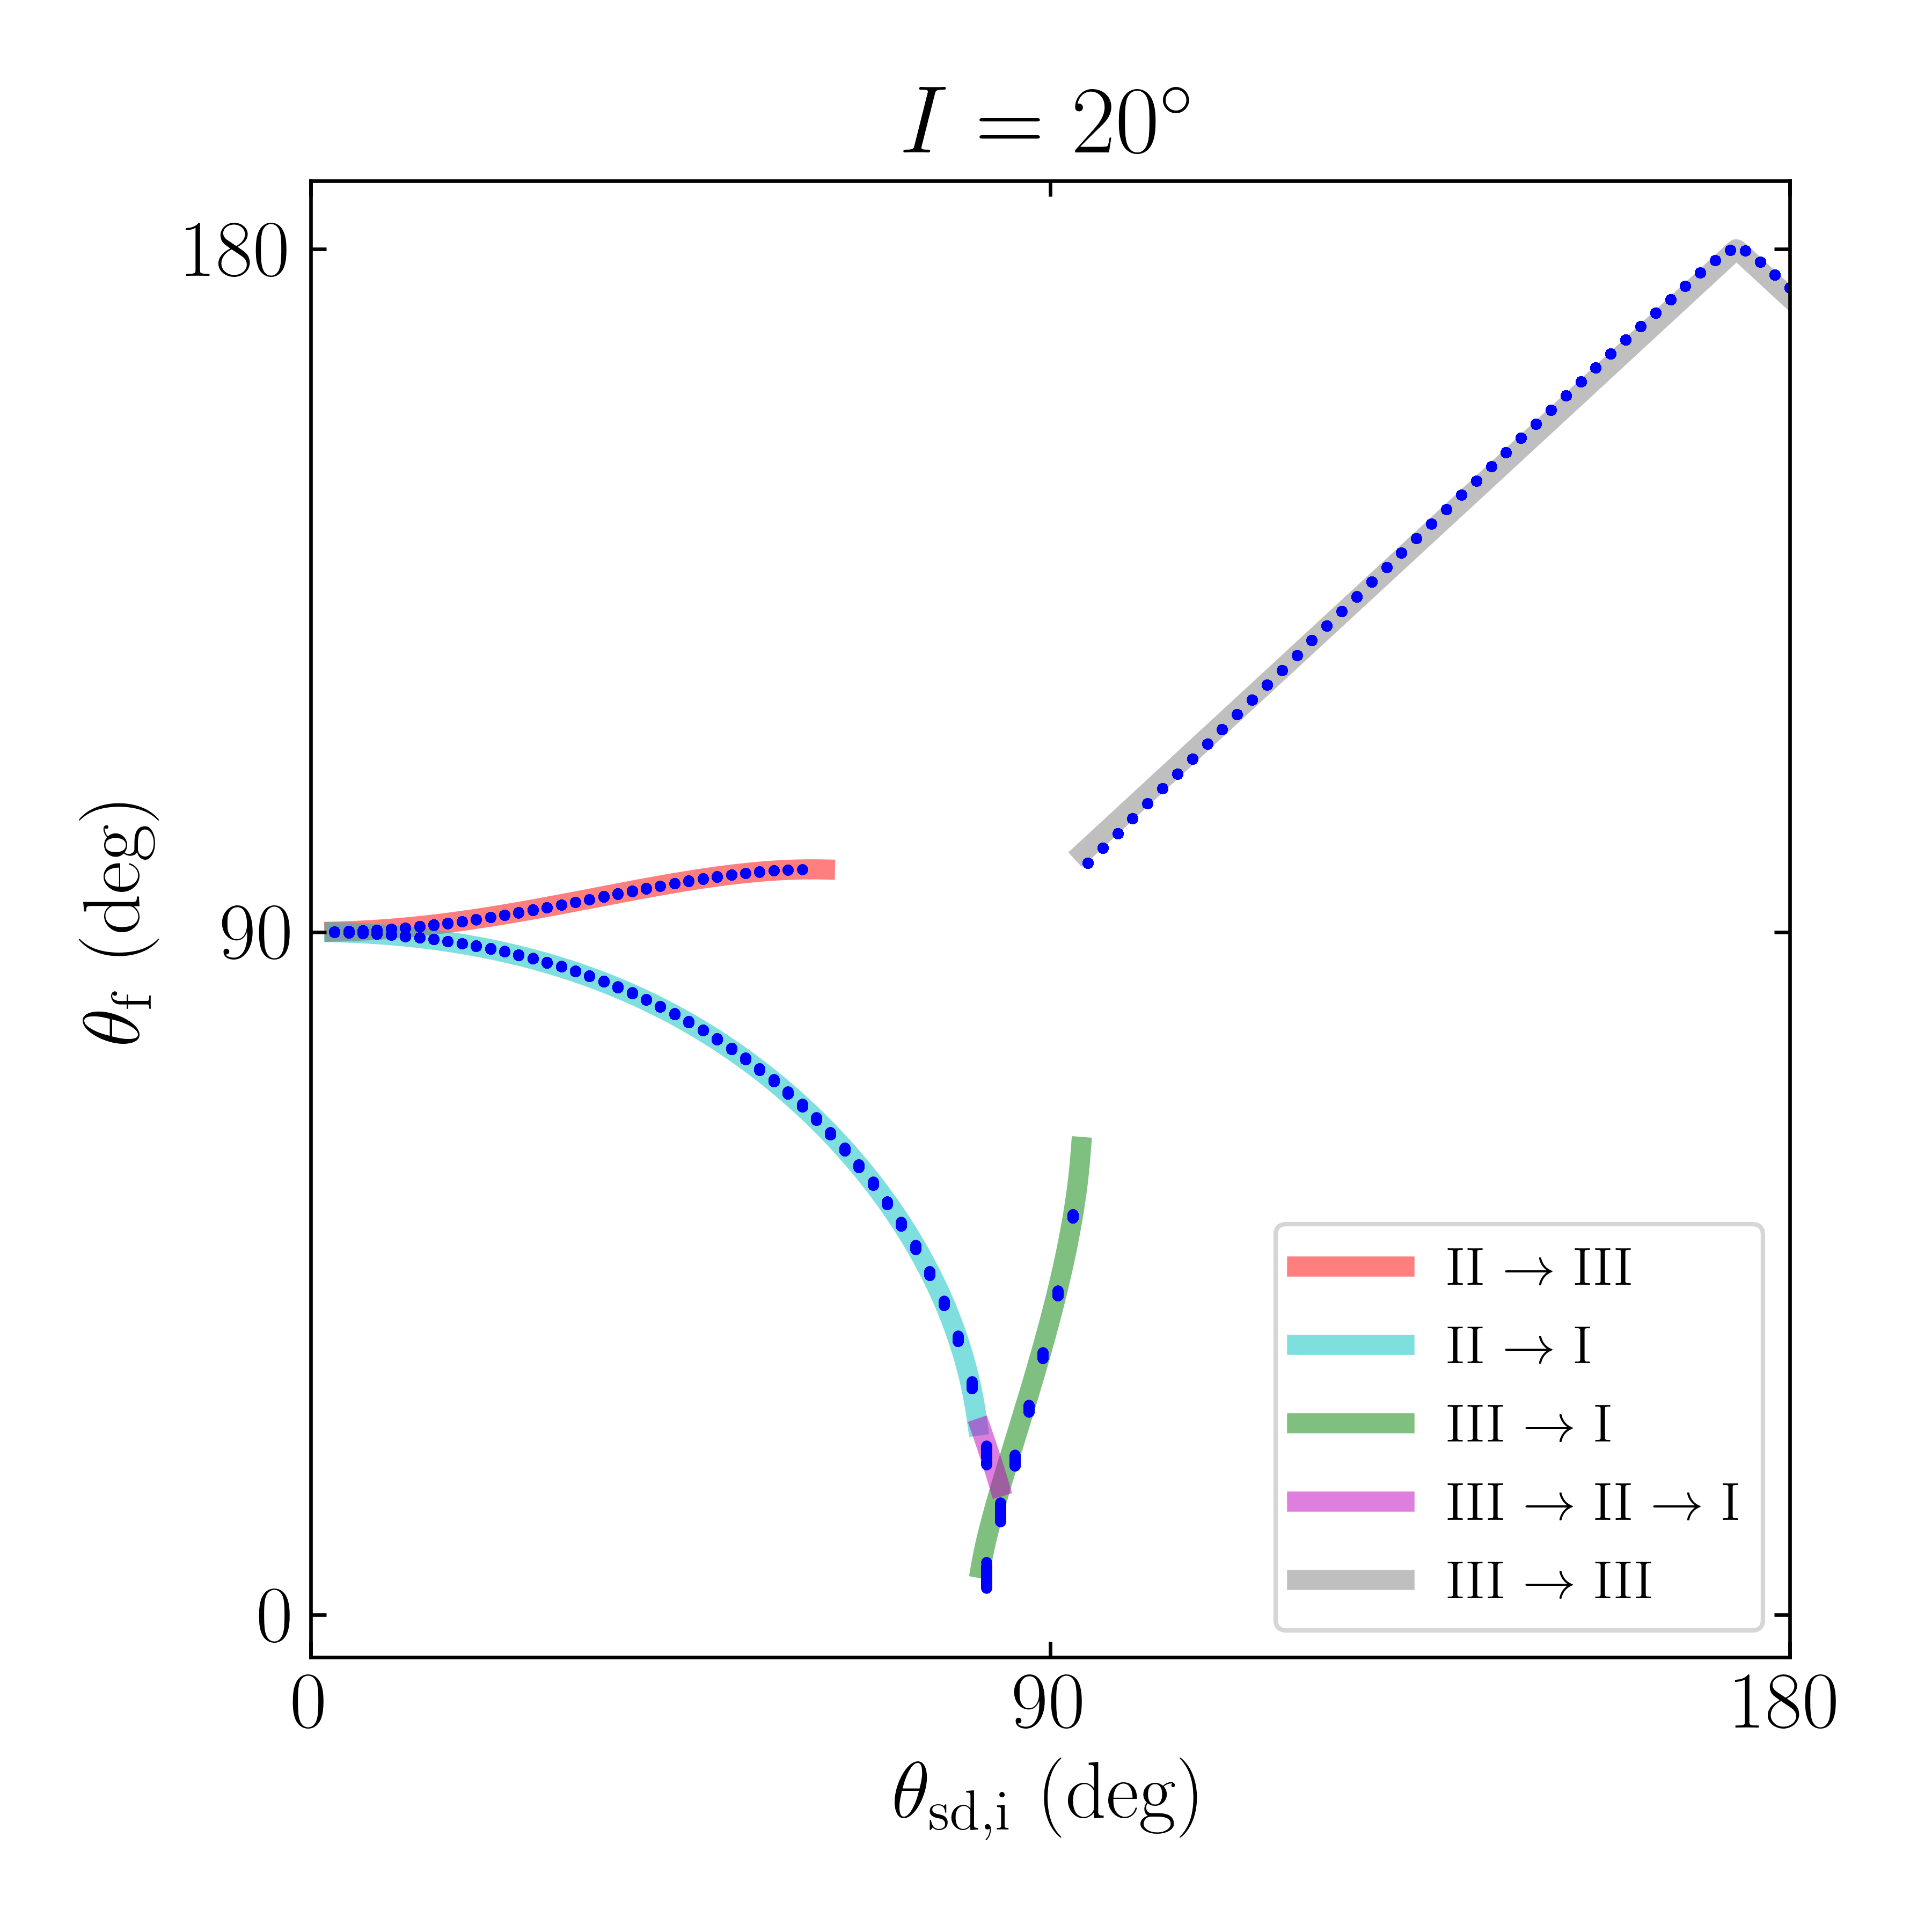
\includegraphics[width=\columnwidth]{../initial/2_toy2/3_ensemble_20_35.png}
    \caption{Same as \autoref{fig:ad_ensemble} but for $I =
    10^\circ$.}\label{fig:3_ensemble_20_35}
\end{figure}

\section{Nonadiabatic Effects}\label{s:nonad}

\subsection{Transition to Non-adiabaticity}

To illustrate the transition to non-adiabaticity, we present three simulations
with increasingly larger values of $\epsilon$ than \autoref{fig:ad_ensemble}
below in \autoref{fig:3_ensemble_05_25} and \autoref{fig:3_ensemble_05_15}.

At first non-adiabaticity manifests as a larger scatter of final obliquities
near the tracks predicted from adiabatic evolution. These scatters first set in
for trajectories starting in zone III, as these cross the separatrix at higher
values of $\theta$ and have a stricter adiabaticity criterion (see
\autoref{eq:ad_constr}).

Later, these large scatters take on band-like structures that seem to persist
across values of $\theta_{sd, i}$; we attribute these to the separatrix crossing
process becoming sensitive to the \emph{phase} of the final
libration/circulation orbit at separatrix crossing. This is equivalent to
separatrix crossing no longer being significantly slower than orbit timescales
and violating the adiabatic assumption.
\begin{figure}
    \centering
    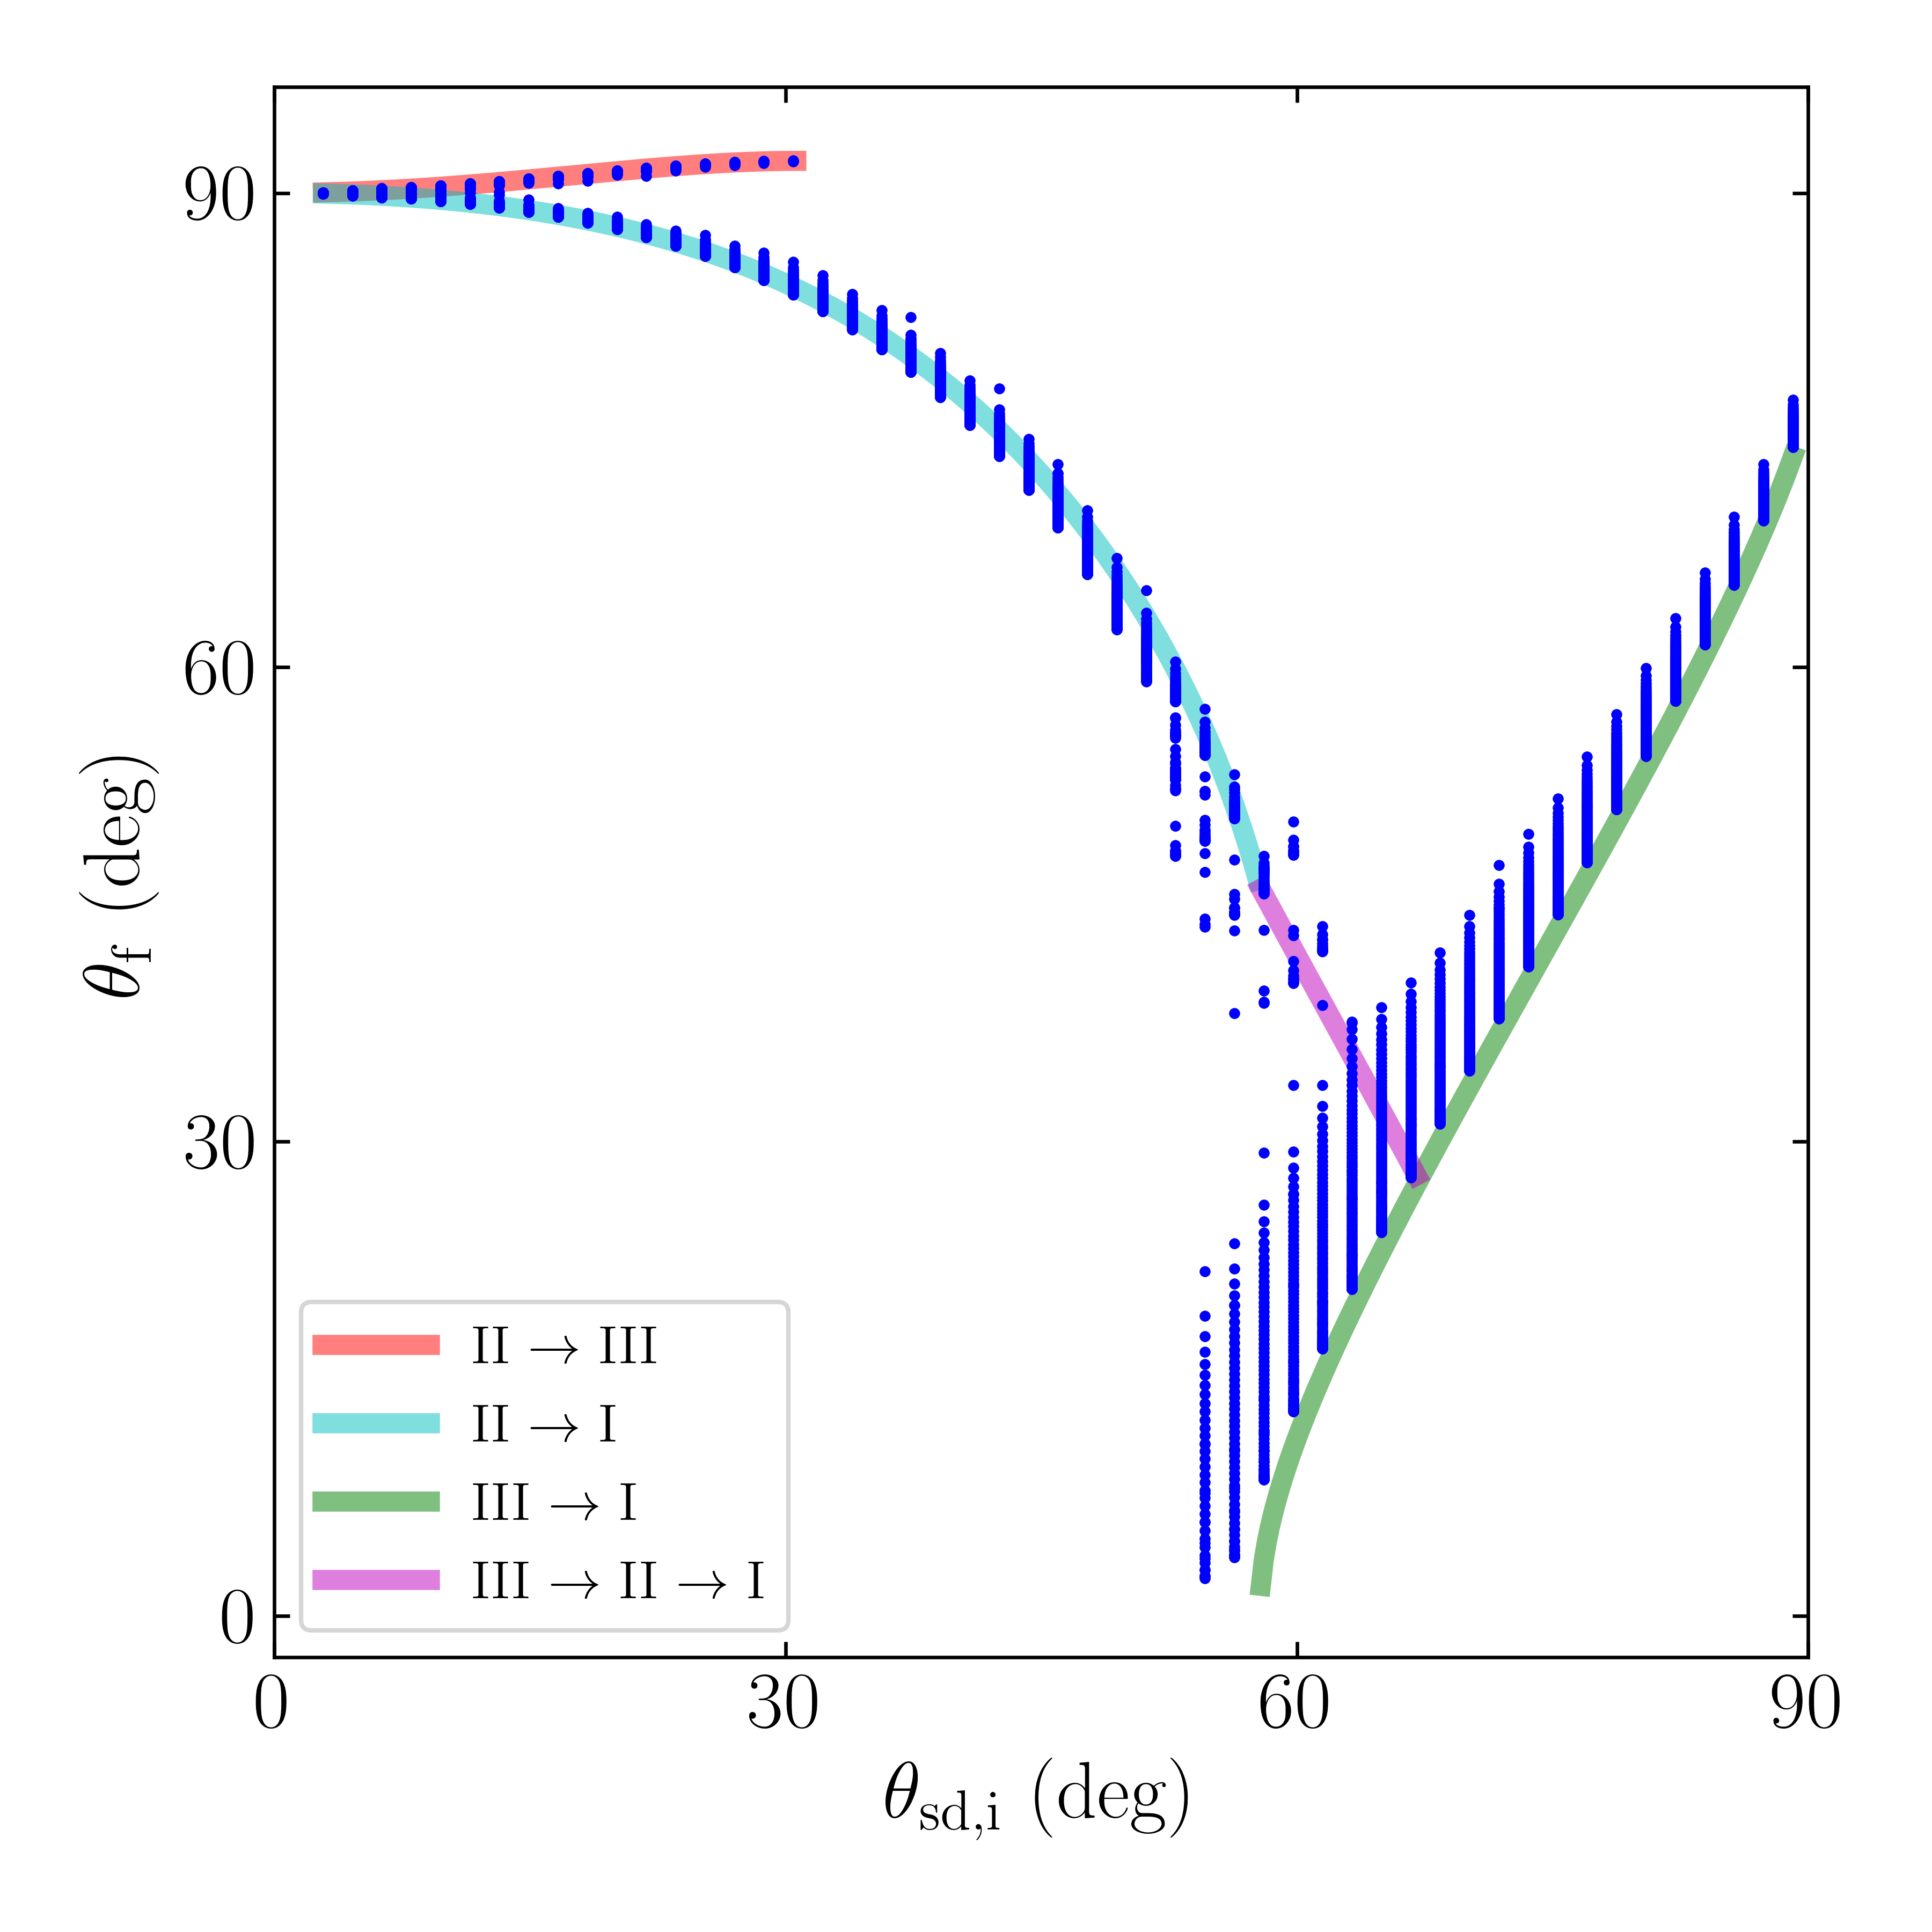
\includegraphics[width=\columnwidth]{../initial/2_toy2/3_ensemble_05_25.png}
    \caption{Same as \autoref{fig:ad_ensemble} but for $\epsilon = 10^{-2.5}$.
    A larger spread from the dynamical tracks is observed in the
    data.}\label{fig:3_ensemble_05_25}
\end{figure}
\begin{figure}
    \centering
    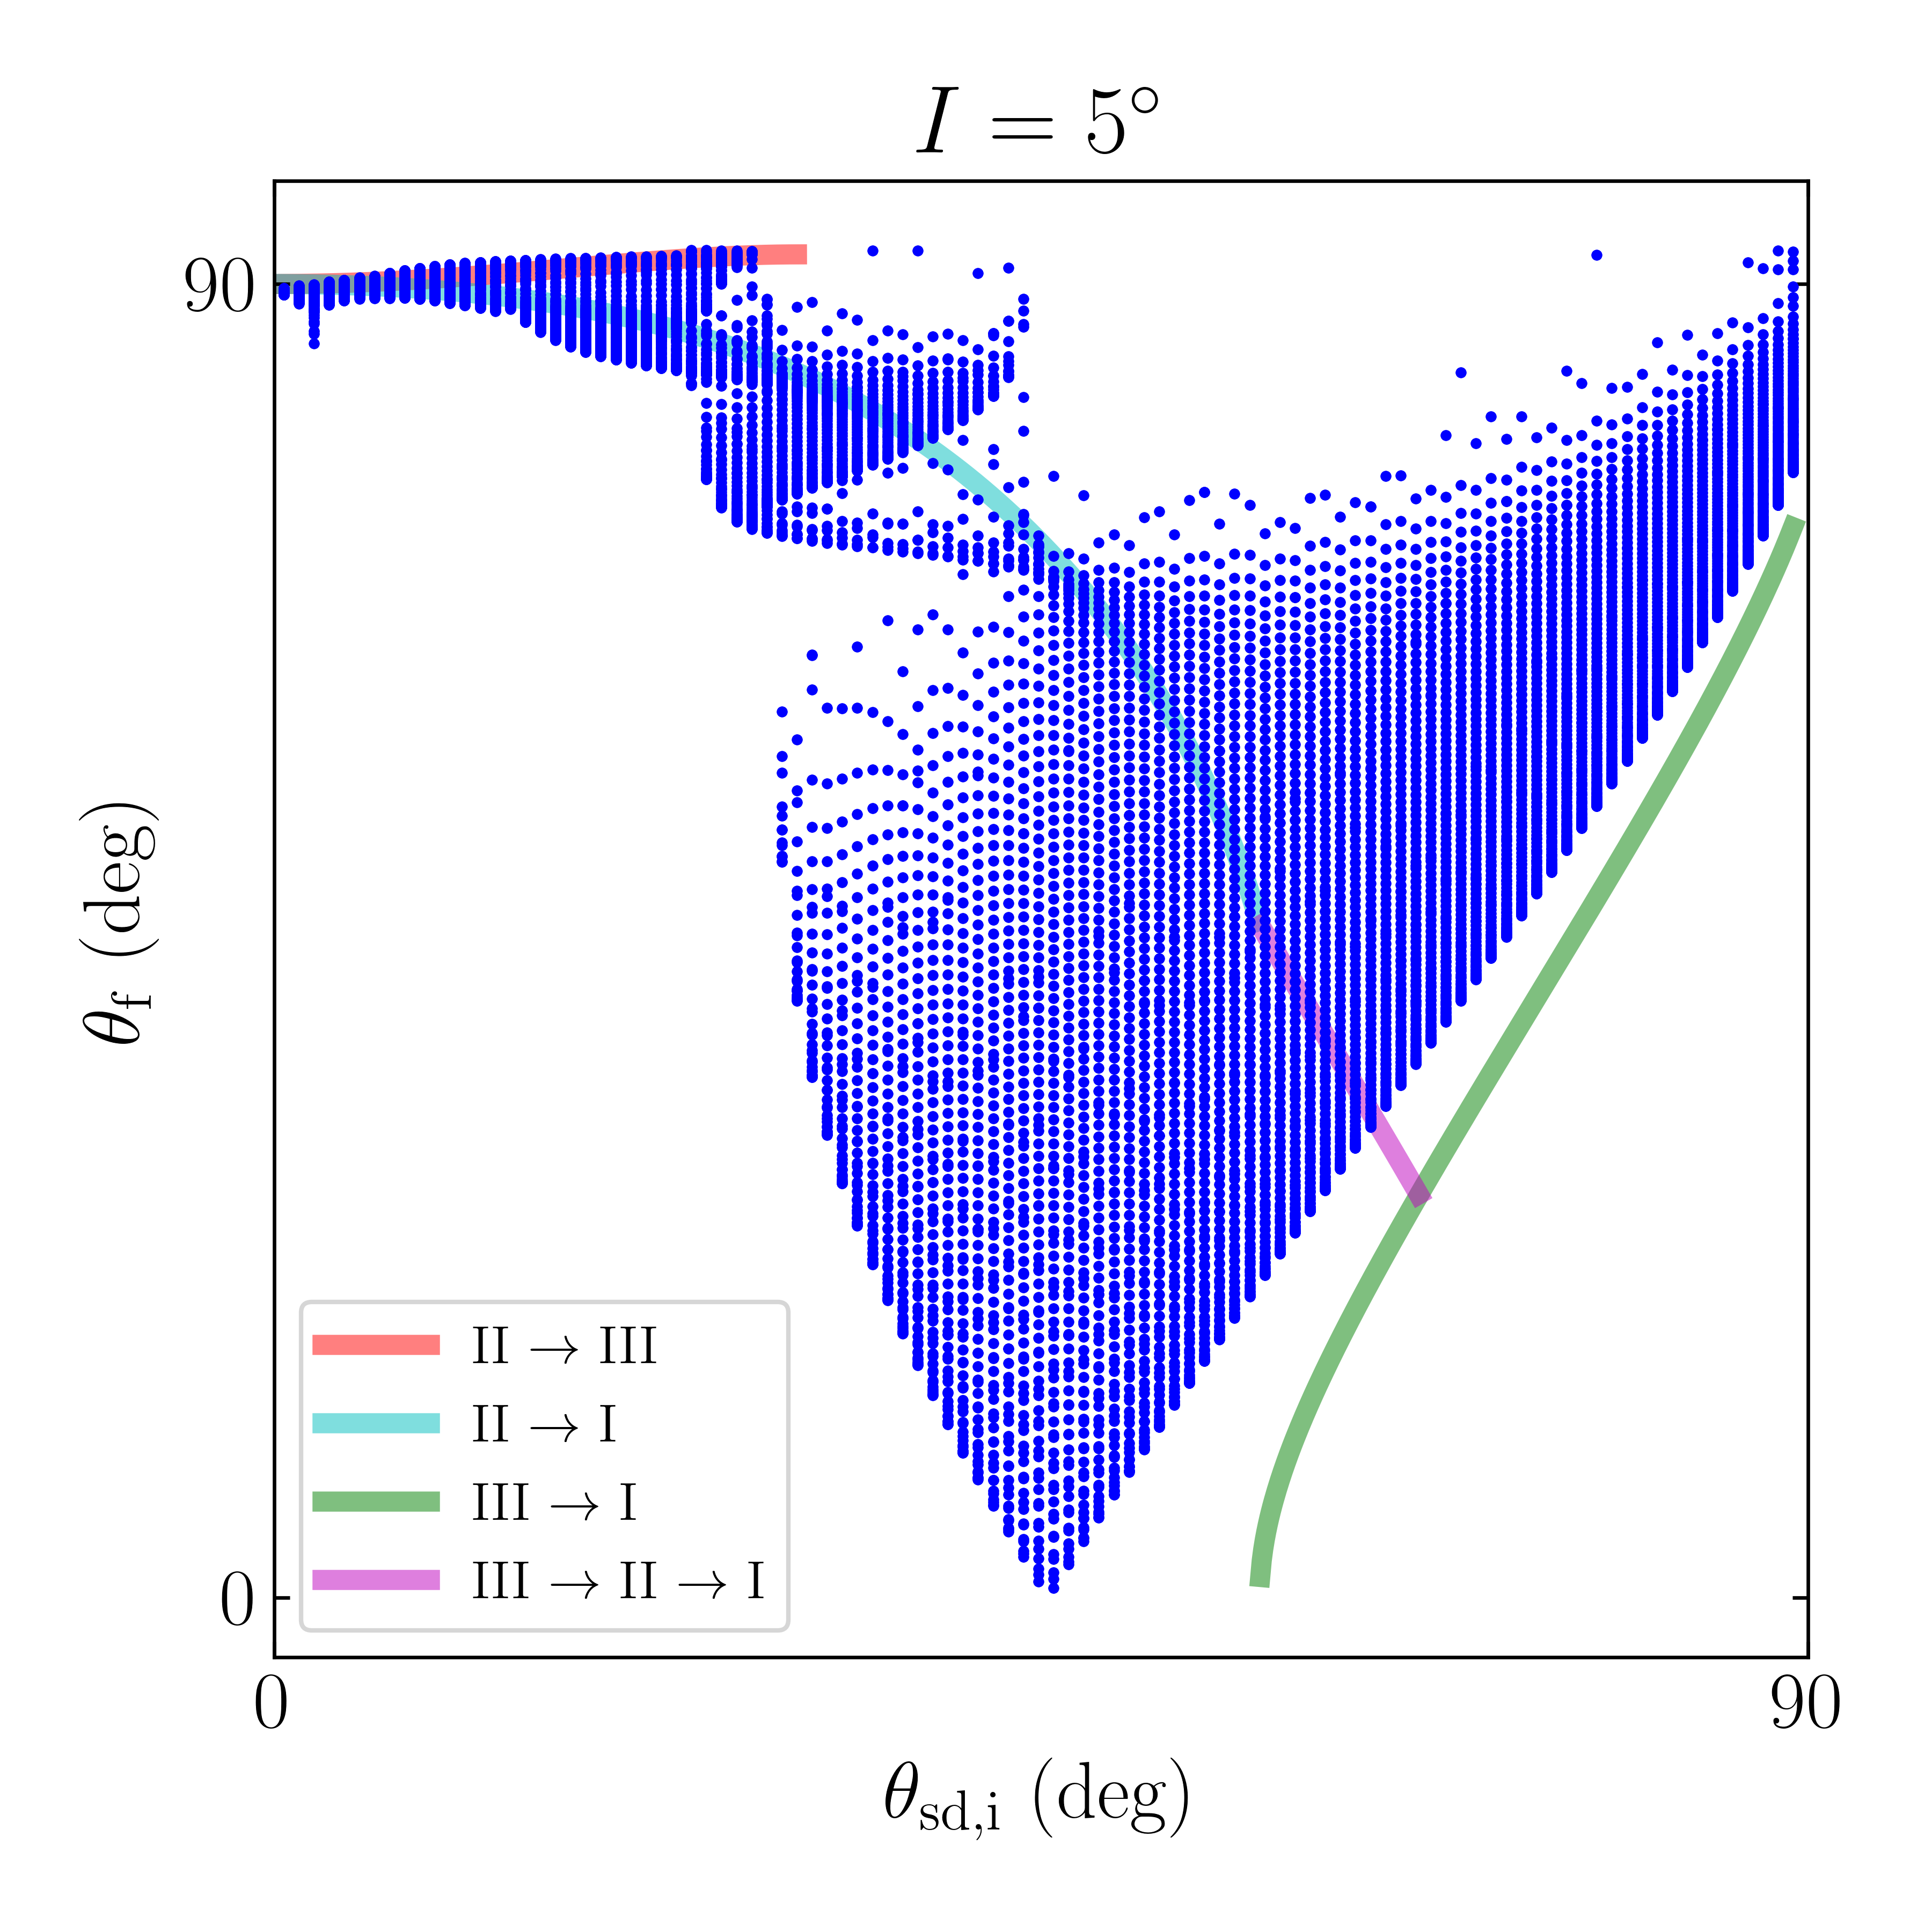
\includegraphics[width=\columnwidth]{../initial/2_toy2/3_ensemble_05_15.png}
    \caption{Same as \autoref{fig:ad_ensemble} but for $\epsilon = 10^{-1.5}$.
    Some small semblance of the evolutionary tracks remains, and the deviations
    appear to have a banded structure. This can be attributed to
    non-adiabaticity ``freezing-in'' the phase of the obliquity variations over
    the final libration/circulation orbit prior to separatrix
    crossing.}\label{fig:3_ensemble_05_15}
\end{figure}

\subsection{Strongly Nonadiabatic Fiducial Trajectory}

A sample trajectory following in the style of \autoref{fig:ad_21} but for
$\epsilon = 0.1$ is provided in \autoref{fig:nonad_traj}.
\begin{figure}
    \centering
    \begin{subfigure}{\columnwidth}
        \centering
        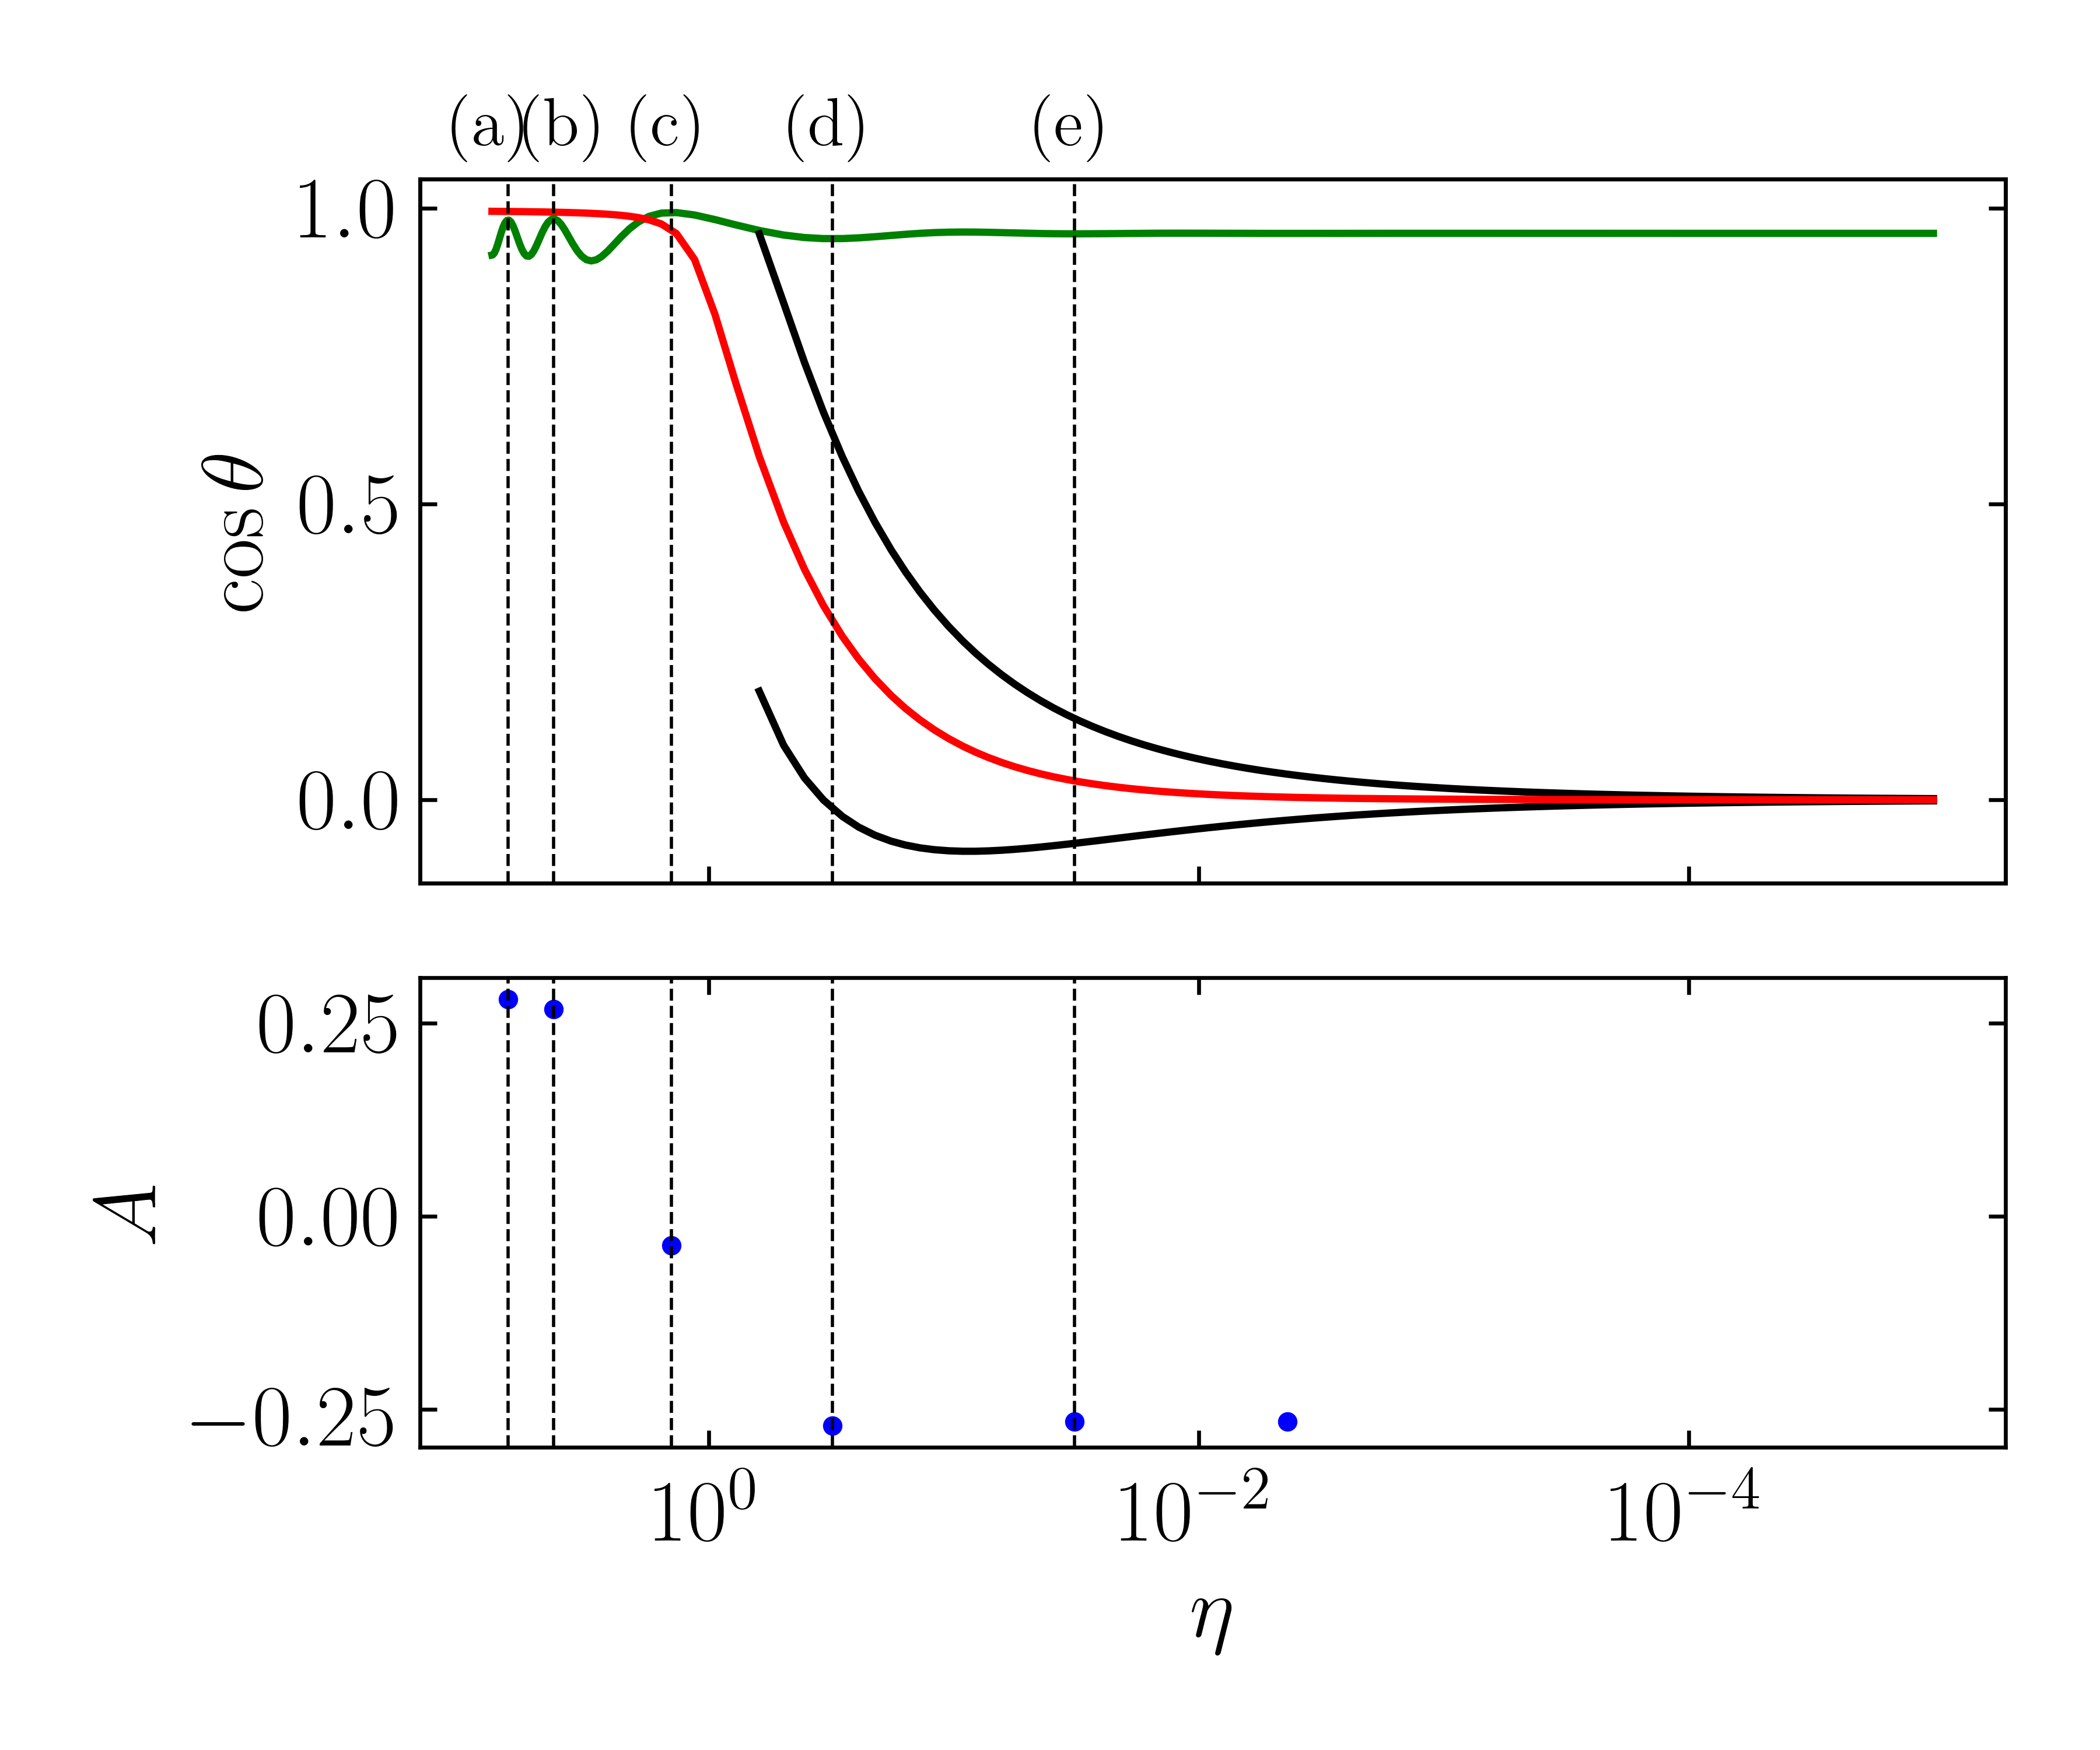
\includegraphics[width=\columnwidth]{../initial/2_toy2/3testo_nonad.png}
    \end{subfigure}
    \begin{subfigure}{\columnwidth}
        \centering
        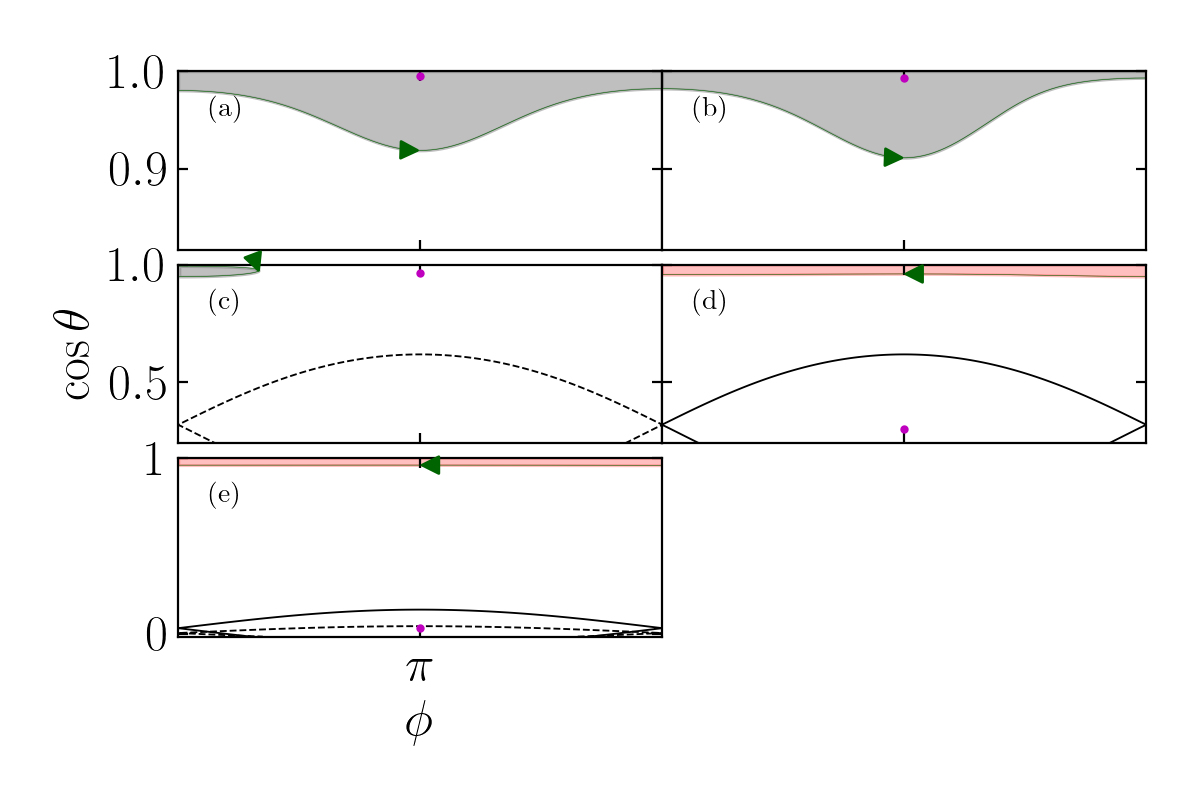
\includegraphics[width=\columnwidth]{../initial/2_toy2/3testo_nonad_subplots.png}
    \end{subfigure}
    \caption{Same as \autoref{fig:nonad_traj} but for a non-adiabatic $\epsilon =
    0.1$. In the top panel of the top plot, it is evident that the libration
    cycle about CS2 is unable to keep up with the swift motion of CS2 as $\eta$
    changes, decreasing the obliquity jump. In the bottom plot, we can see that
    individual orbits do not lie along level curves of the Hamiltonian, a
    further consequence of violating adiabaticity.}\label{fig:nonad_traj}
\end{figure}

\subsection{Dynamical Outcomes}

A formula for $\theta_{f}$ assuming $\theta_{sd, i} = 0$ initially can be
given (see \autoref{ss:app_transition})
\begin{equation}
    \theta_{f}\p{\theta_{sd, i} = 0} = \sqrt{\frac{2\pi \Omega}{\epsilon}}
        \tan I.\label{eq:nonad_q_f}
\end{equation}
We can naively generalize this by recognizing that any nonzero $\theta_{sd, i}$
manifests as obliquity variations as $\hat{s}$ librates about $\hat{l}_d$, and
these oscillations are ``frozen in'' when the disk dissipates. Thus,
\begin{equation}
    \theta_{f}\p{\theta_{sd, i}} \in \sqrt{\frac{2\pi \Omega}{\epsilon}}
        \tan I \pm \theta_{sd, i}.\label{eq:nonad_q_f_dist}
\end{equation}

We present the results of simulations for using $\epsilon = 0.3$ in
\autoref{fig:nonad_3_ensemeble}.
\begin{figure}
    \centering
    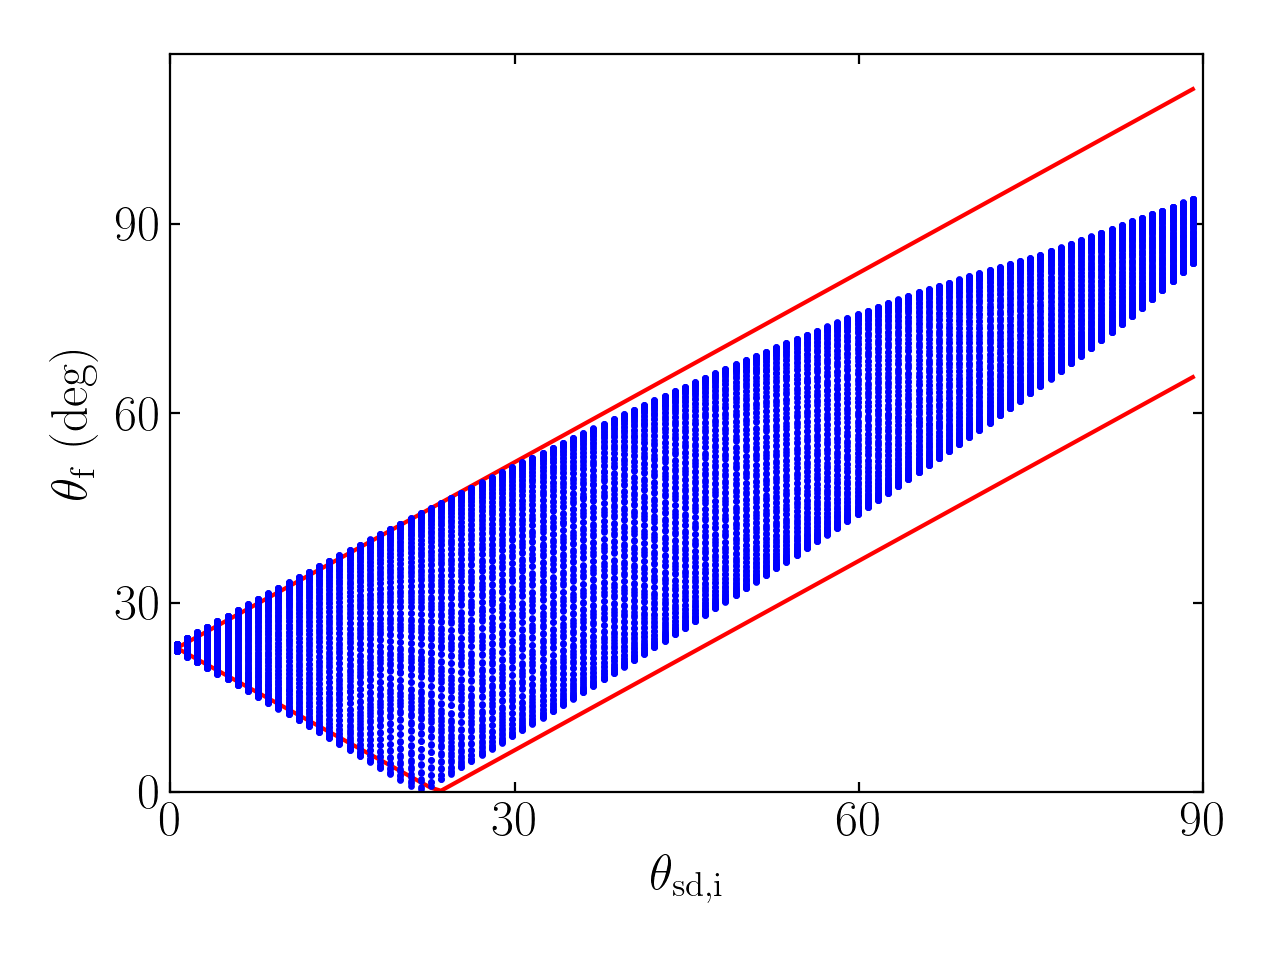
\includegraphics[width=\columnwidth]{../initial/2_toy2/3_ensemble_05_05.png}
    \caption{$\theta_{ f}\p{\theta_{sd, i}}$ at $\epsilon = 0.3$, firmly in
    the non-adiabatic regime. Note the clear double-valuedeness has disappeared,
    as have distinct dynamical tracks. The red dotted line presents the
    analytical prediction given by
    \autoref{eq:nonad_q_f_dist}.}\label{fig:nonad_3_ensemeble}
\end{figure}

The agreement of \autoref{eq:nonad_q_f} at fixed $I$ for varying $\epsilon$ is
shown in \autoref{fig:nonad_3_scan}. Note that $\epsilon \to 0$ recovers the
adiabatic regime. The deviation of $\theta_f$ from the analytical prediction
within the adiabatic regime is indeed due to adiabatic effects becoming
dominant; compare to \autoref{fig:nonad_3_scan_20} where little deviation is
observed until $\theta_f \approx 90^\circ$.
\begin{figure}
    \centering
    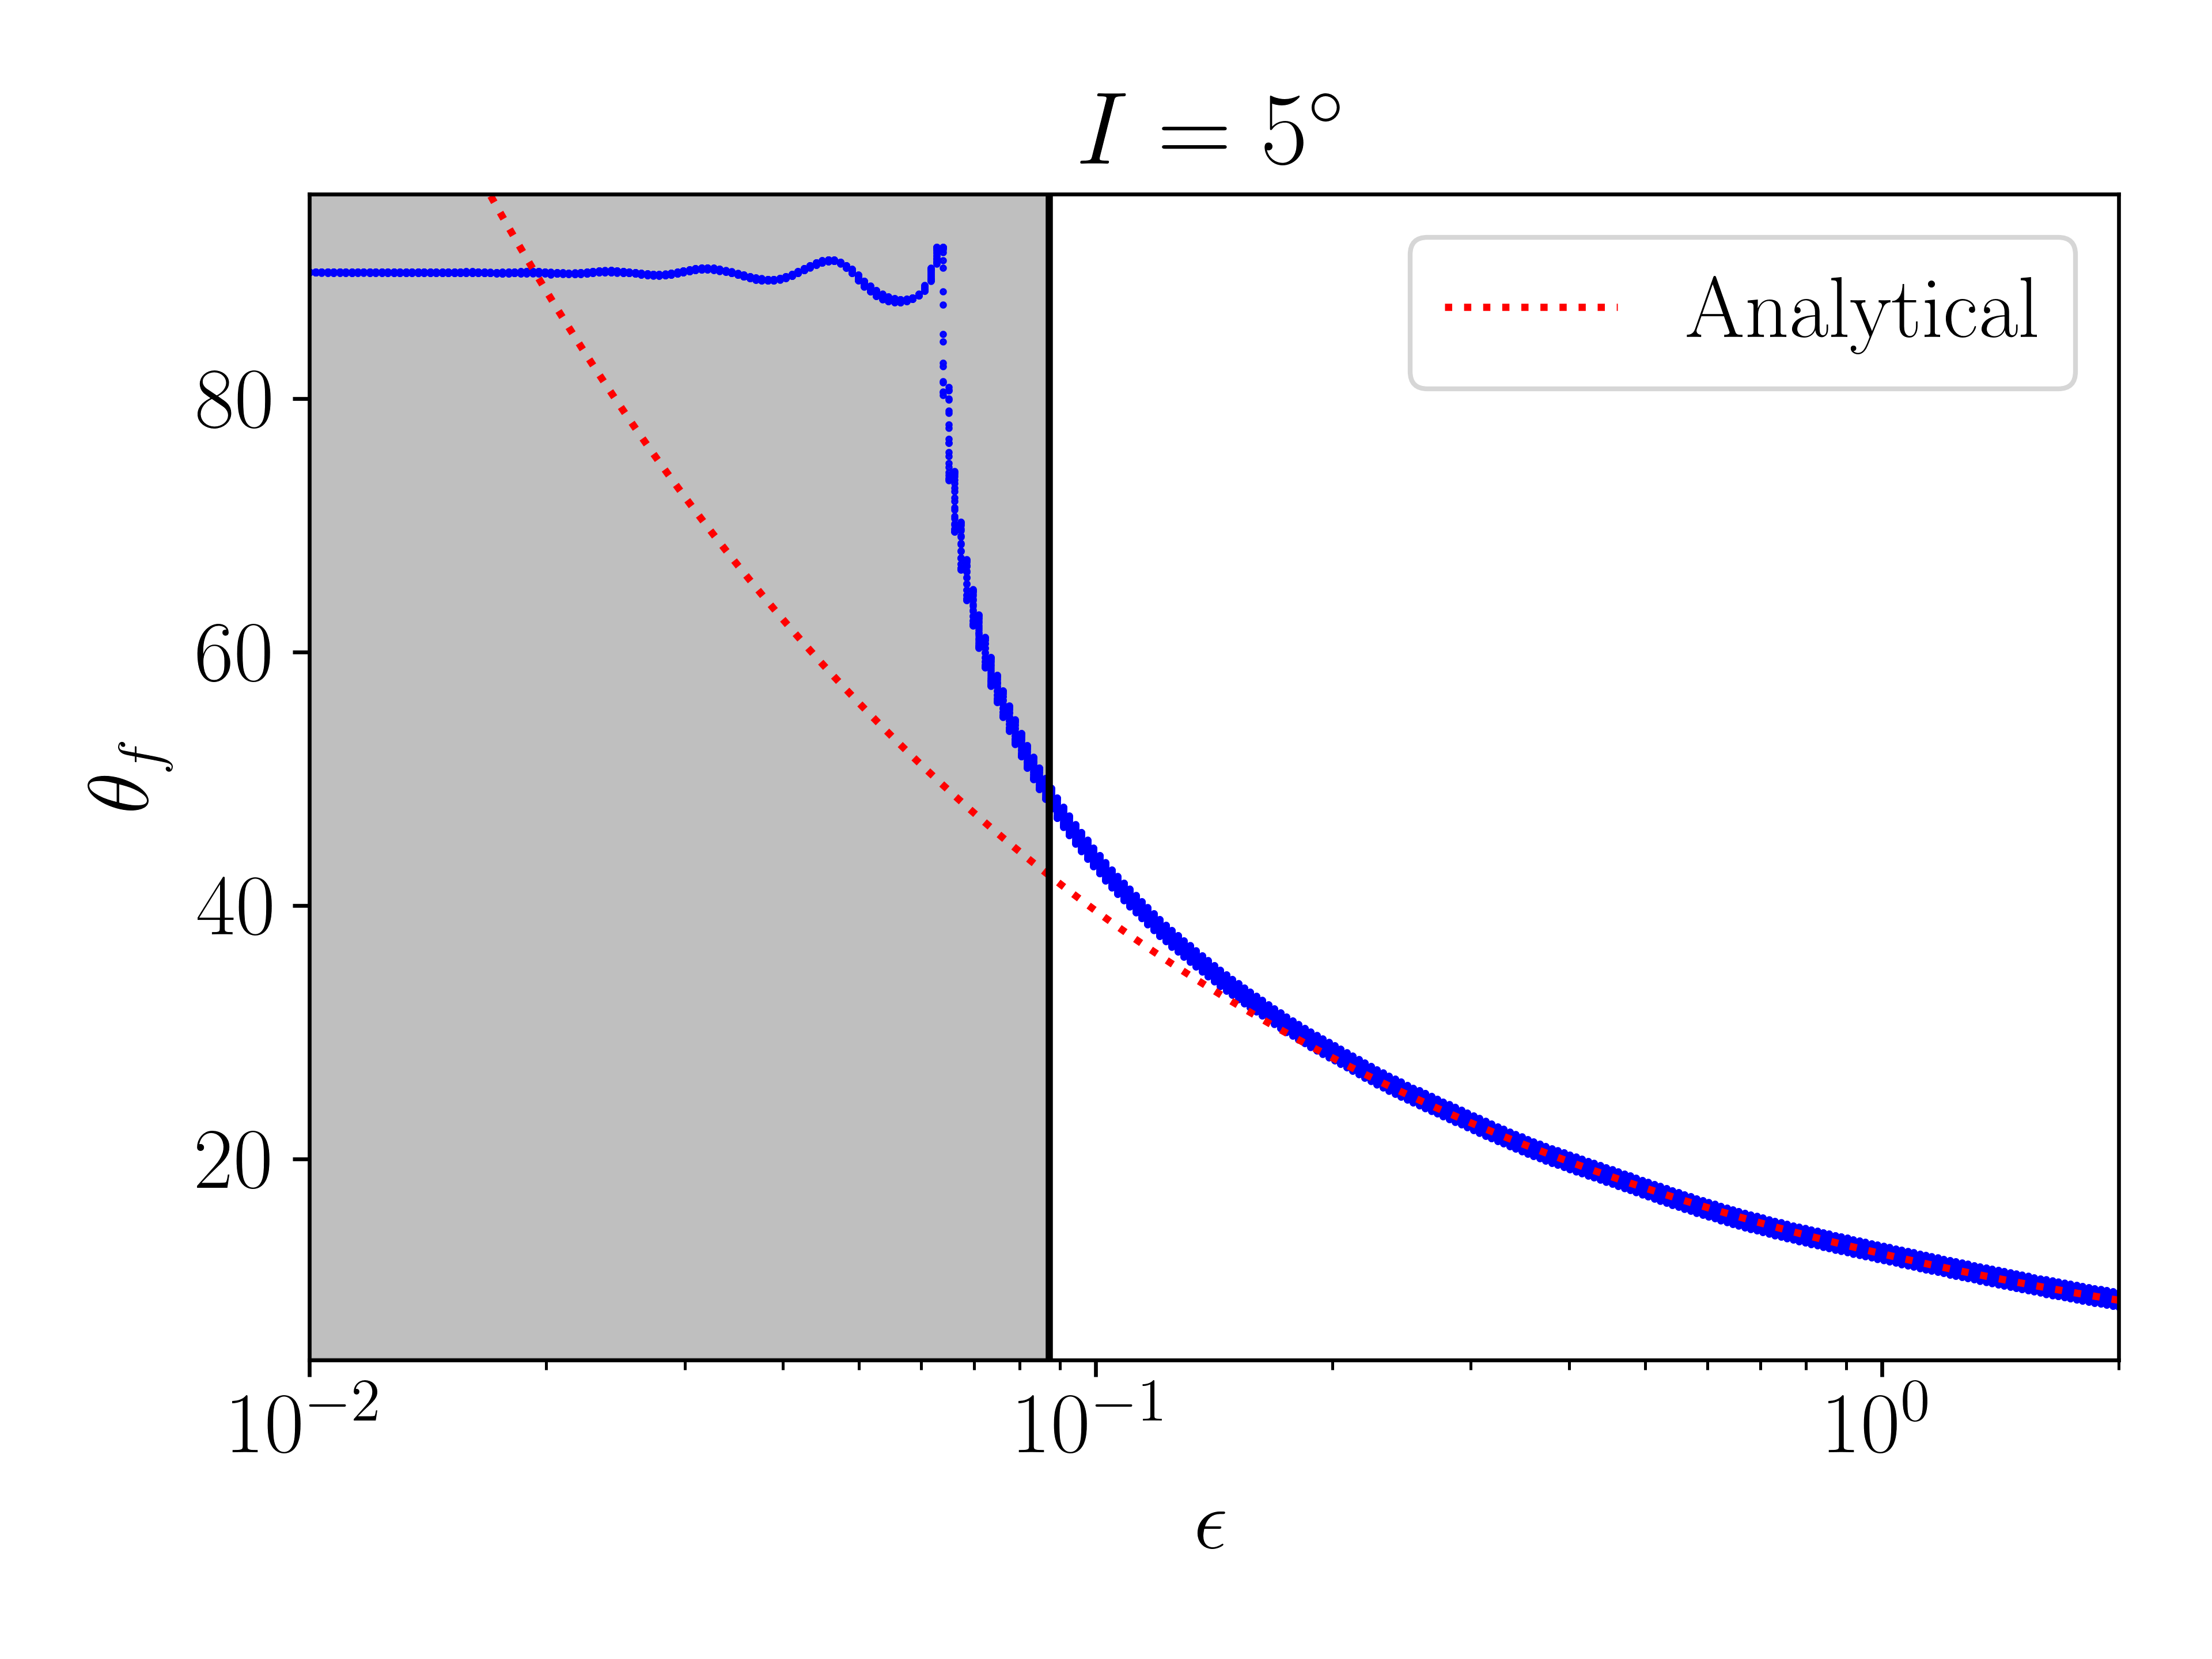
\includegraphics[width=\columnwidth]{../initial/2_toy2/3scan.png}
    \caption{Plot of $\theta_{ f}\p{\theta_{sd, i} = 0}$ as a function of
    $\epsilon$, where $I = 5^\circ$. Overplotted in the red line is
    \autoref{eq:nonad_q_f}, which is in good agreement for $\epsilon \gtrsim
    0.1$ the non-adiabatic regime, while $\theta_{ f} \approx 90^\circ$ in
    the adiabatic regime.}\label{fig:nonad_3_scan}
\end{figure}
\begin{figure}
    \centering
    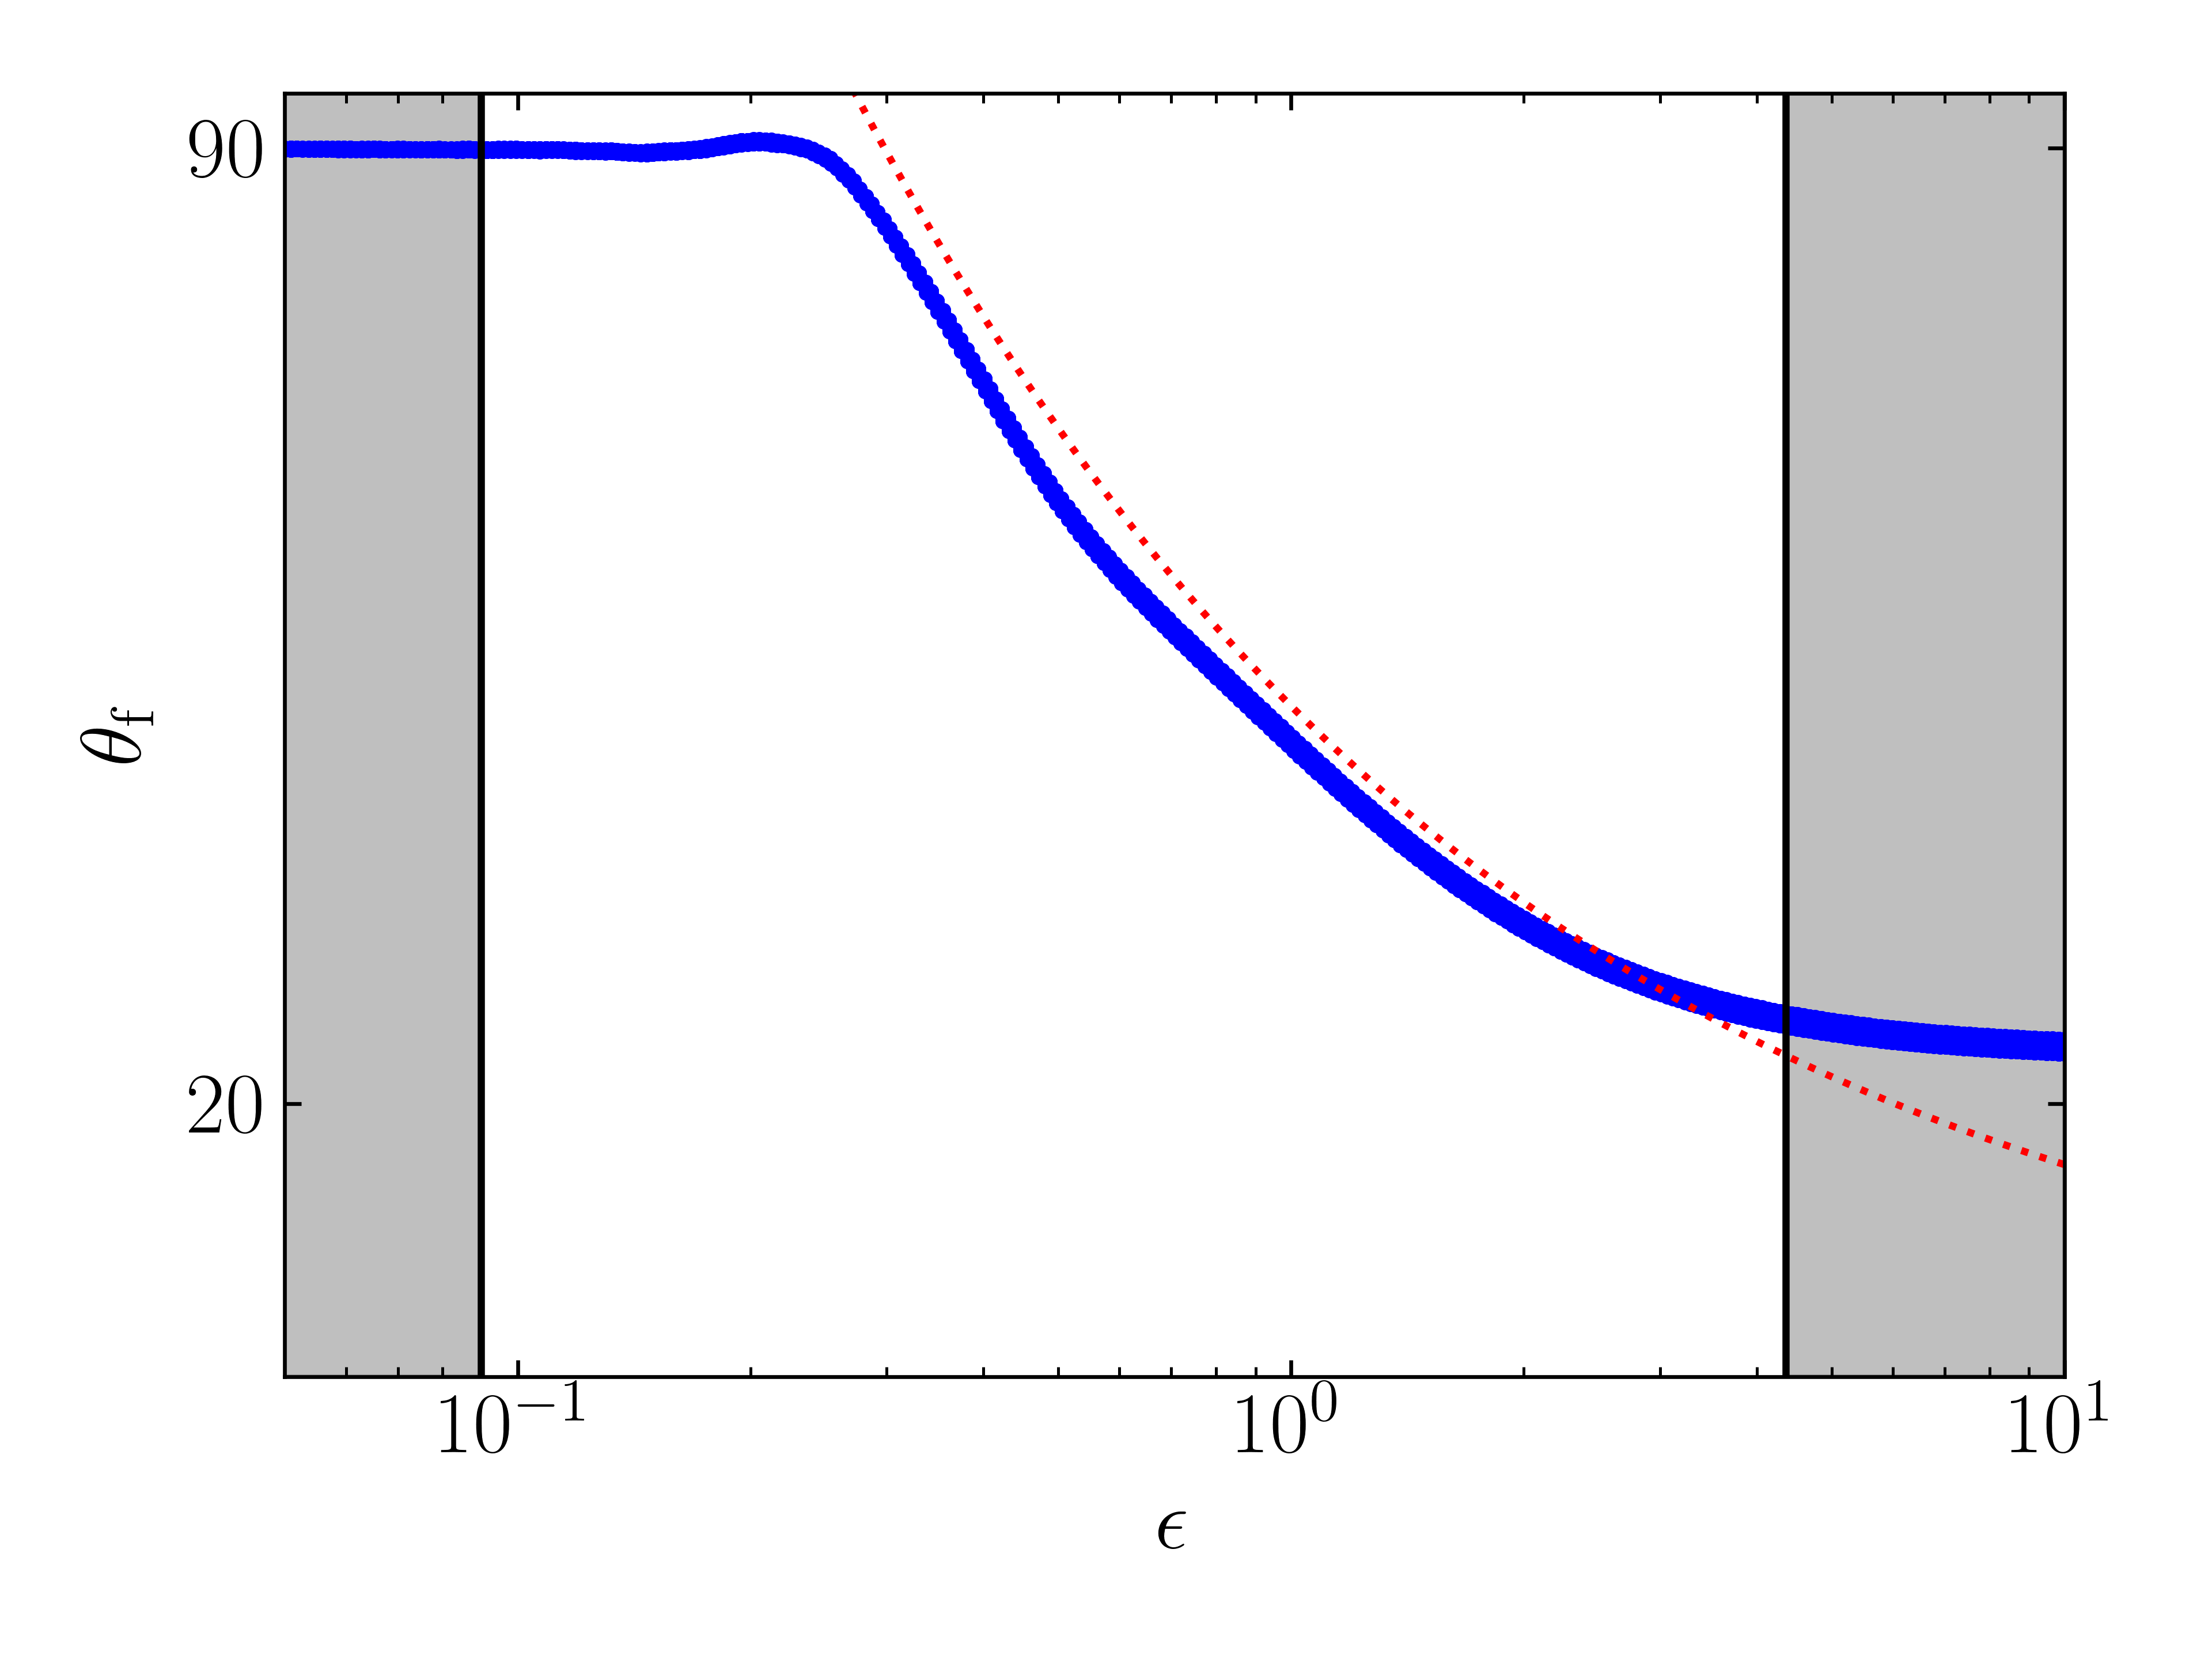
\includegraphics[width=\columnwidth]{../initial/2_toy2/3scan_20.png}
    \caption{Same as \autoref{fig:nonad_3_scan} but for $I=20^\circ$. Note that
    the analytical prediction is accurate until $\theta_f \approx 90^\circ$,
    which occurs before the transition to the adiabatic
    regime.}\label{fig:nonad_3_scan_20}
\end{figure}

\bibliographystyle{mnras}
\bibliography{Su_sep_cross}

% \clearpage
% \onecolumn
\appendix

\section{Adiabatic Evolution}

\subsection{Analytic $\theta_f$ for small $\theta_{sd,
i}$}\label{ss:app_transition}

In this section, we will use approximations valid for small $\eta$ to derive
analytic expressions for the final obliquities and associated probabilities for
the $II \to I, II \to III$ tracks that govern behavior at small $\theta_{sd,
i}$.

We first seek a simple parameterization for the separatrix. We first solve for
equilibria of the equation of motion \autoref{eq:dsdt_base} to compute the
coordinates for Cassini State 4:
\begin{equation}
    \cos \theta_4 \approx \frac{\mu \cos I}{1 - \eta \sin I}.
\end{equation}
Note that $\phi_4 = 0$. Then, the separatrix is the level curve of the
Hamiltonian intersecting CS4, so it satisfies $\mathcal{H}\p{\theta_{sep}(\phi),
\phi} = \mathcal{H}\p{\theta_4, \phi_4}$. This solves to be approximately
\begin{equation}
    \cos \theta_{sep}(\phi) \approx \cos \theta_4 \pm
        \sqrt{2\eta \sin I\p{1 - \cos \phi}}.
\end{equation}
Integration of the phase area enclosed by the two legs of the separatrix then
yields
\begin{equation}
    A_{II}(\eta) \approx 16\sqrt{\eta \sin I}.\label{eq:a_approx}
\end{equation}
This, in conjunction with \autoref{eq:henrard_hop}, is sufficient to compute
$\theta_f\p{\theta_{sd, i}}$ for zone II initial conditions.

\begin{itemize}
    \item For a given $\theta_{sd, i}$, we know that if $\eta \to \infty$ then
        the trajectory executes simple libration about $\hat{l}_d$, and so $A =
        2\pi\p{1 - \cos \theta_{sd, i}} \approx \pi \theta_{sd, i}^2$. This
        then implies $\eta_\star$ must be the solution to $A_{II}(\eta_\star) =
        A$, or
        \begin{align}
            \eta_\star &\approx \p{\frac{2\pi\p{1 - \cos \theta_{sd,i}}}{
                        16}}^2 / \sin I,\nonumber\\
                    &\approx \p{\frac{\pi \theta_{sd, i}^2}{16}}^2/\sin I.
        \end{align}

    \item Upon separatrix encounter, a transition to either zone I or zone III
        occurs. These can be calculated to have associated probabilities (using
        the approximate area \autoref{eq:a_approx})
        \begin{align}
            \Pr_{II \Rightarrow I} &\approx \frac{2\pi
                \eta_{\star} \cos I + 4\sqrt{\eta_{\star}\sin
                I}}{8\sqrt{\eta_{\star}\sin I}},\\
            \Pr_{II \Rightarrow III} &\approx \frac{-2\pi
                \eta_{\star} \cos I + 4\sqrt{\eta_{\star}\sin
                I}}{8\sqrt{\eta_{\star}\sin I}}.
        \end{align}

    \item Upon a transition to zone I or zone III, the final obliquities can be
        predicted by observing the final adiabatic invariant $A_f =
        -A_I(\eta_\star)$ in the zone I case and $A_f = A_I(\eta_\star) +
        A_II(\eta_\star)$ in the zone III case. As $\eta \to 0$, these
        correspond to obliquities
        \begin{align}
            \cos \theta_{f, II \Rightarrow I} &\approx
                \p{\frac{\pi \theta_{sp, i}^2}{16}}^2 \cot I
                    + \frac{\theta_{sp, i}^2}{4},\\
            \cos \theta_{f, II \Rightarrow III} &\approx
                \p{\frac{\pi \theta_{sp, i}^2}{16}}^2 \cot I
                    - \frac{\theta_{sp, i}^2}{4}.
        \end{align}
        These are the black dotted lines overplotted in
        \autoref{fig:ad_ensemble}.
\end{itemize}

\section{Nonadiabatic Evolution}\label{s:nonad_app}

We present a single result, the derivation of \autoref{eq:nonad_q_f}. We take
\autoref{eq:dsdt_base} and choose coordinate axes such that $\hat{l} = \hat{z},
\hat{l}_d = \hat{z} \cos I + \hat{x}\sin I$, then we obtain
\begin{equation}
    \rd{\hat{s}}{t} = \s{
        \p{\eta \cos I - 1}\hat{z} + \eta \sin I \hat{x}} \times \hat{s}.
\end{equation}

Now, let's assume that $s_z \approx \cos I$ throughout the evolution of $\hat{s}$
(note that $\theta_{sd, i} = 0$ implies the initial $s_z = \cos I$). Then let's
examine the evolution of quantity $S = s_x + is_y$ instead:
\begin{equation}
    \rd{S}{t} = i\p{\eta\cos I - 1}S - i \eta \sin I\cos I.\label{eq:nonad_ode}
\end{equation}
Now this is a first-order ODE in $S$, albeit complex, which can be solved via
an integrating factor
\begin{align}
    \Phi(t) &\equiv \int_{-\infty}^t \p{1 - \eta(t') \cos I}
        \mathrm{d}t',\\
    \at{S(t) e^{i\Phi(t)}}_{-\infty}^t
        &= \int\limits_{-\infty}^t e^{i\Phi(t')}
            \p{-i\eta(t')\sin I\cos I}\;\mathrm{d}t'\label{eq:nonad_int}
\end{align}
We now invoke stationary phase, asserting that $e^{i\Phi(t)}$ is dominated by
its contribution where $\dot{\Phi} = 0$ (the phases add constructively). But
$\dot{\Phi} = 0$ is where $1 - \eta\cos I = 0$, or where $\eta\cos I = 1$.

Now at this point, let's choose $\eta(0) = 1/\cos I, \at{\rd{\eta}{t}}_{t=0} =
-\epsilon/\cos I$. Then we expand near $t = 0$ so
\begin{align*}
    \Phi(t) &\approx \Phi(0) + \frac{1}{2}\ddot{\Phi}t^2,\\
        &\approx \Phi(0) + \frac{1}{2}\epsilon t^2,\\
    \int\limits_{-\infty}^t e^{i\Phi(t')}\eta(t')\;\mathrm{d}t'
        &\approx
        \begin{cases}
            0 & t < 0,\\
            \frac{1}{\cos I}e^{i\Phi(0)}\int\limits_{-\infty}^\infty
                \exp\s{\frac{i}{2}\epsilon t^2}\;\mathrm{d}t
                & t > 0.
        \end{cases}\\
    \int\limits_{-\infty}^\infty
                \exp\s{\frac{i}{2}\epsilon t^2}\;\mathrm{d}t
        &= \int\limits_{-\infty}^\infty e^{-\tau^2}\;\mathrm{d}\tau
            \sqrt{\frac{2}{i\epsilon}},\\
        &= \sqrt{\frac{2\pi}{i\epsilon}}.
\end{align*}

Now, it should be noted that $e^{i\Phi}$ is just a phase; all we really care
about is $\abs{S} = \sqrt{1 - s_z^2}$. Thus, taking the absolute value of both
sides of \autoref{eq:nonad_int}, assuming $S\p{-\infty} \ll S\p{+\infty}$ and
noting $\theta_f \approx \abs{S}(+\infty)$, we obtain
\begin{equation}
    \theta_f = \tan I\cos I\sqrt{\frac{2\pi}{\epsilon}}.\label{eq:nonad_dong}
\end{equation}

It should be noted that this calculation breaks down in two ways:
\begin{itemize}
    \item If the evolution of $\hat{s}$ is adiabatic, then it is invalid to
        assume $s_z$ is approximately constant in time, as many
        circulation/libration orbits can ensue. Only when the driving is
        sufficiently impulsive that the evolution dominates the change in $s_z$
        is this calculation valid.

    \item If $\abs{S\p{-\infty}} \sim \abs{S\p{+\infty}}$, then taking the
        absolute value of both sides of \autoref{eq:nonad_int} no longer simply
        yields $\abs{S}\p{+\infty}$. This corresponds to the extreme limit
        where $\eta$ changes so suddenly that $\hat{s}$ has no time to respond
        and remains roughly unchanged as $\eta \to 0$. This is accommodated by
        noting $\theta_f \geq \theta_{sd, i}$, so the correct estimate can be
        roughly amended
        \begin{equation}
            \theta_f \simeq \min\p{\tan I\cos I\sqrt{\frac{2\pi}{\epsilon}},
                \theta_{sd, i}}.
        \end{equation}
\end{itemize}

\label{lastpage} % chktex 24
\end{document}
